\def\auth{Carlos Salinas}%
\def\tight{MA 519: Homework, Midterms and Practice Problems Solutions}%
\def\short{MA519-HW-ALL}%
\def\class{MA 51900}%
\def\subject{elementary probability}%
\def\email{salinac@purdue.edu}%

\documentclass{article}
\usepackage{geometry}

%% Base customization and variables
\usepackage{preamble}

%% Footnote style
\renewcommand*{\thefootnote}{\fnsymbol{footnote}}

%% Hyperref setup
\hypersetup{%
  breaklinks,%
  colorlinks=true,%
  linkcolor=black,%
  citecolor=black,%
  filecolor=black,%
  menucolor=black,%
  runcolor=black,%
  urlcolor=black,%
  pdftitle={\short},%
  pdfauthor={\auth},%
  pdfkeywords={\subject},%
  pdfsubject={\class},%
  % pageanchor={false},%
  unicode
}

%% Graphics path as it says
\graphicspath{{figures/}}

\begin{document}%

% \author{\href{mailto:\email}{\auth}}
\author{\textti\auth}%
\title{\textti\tight}%
\date{\textti{Last compiled: \today}}%
\maketitle%
\tableofcontents%
\numberwithin{equation}{subsection}

%% DasGupta's homework
\begin{problem}[Handout 1, \# 5 \protect{[Feller Vol.\@ 1]}]
  A closet contains five pairs of shoes. If four shoes are selected at
  random, what is the probability that there is at least one complete pair
  among the four?
\end{problem}
\begin{solution}
  Let \(\Omega\) denote the sample space and \(A\) denote the event that at
  least \(1\) complete pair of shoes is among the \(4\). We can reduce the
  problem of finding \(P(A)\) into finding the probabilities of the
  mutually exclusive events
 \[
   A_1\defeq\bigl\{\,\text{exactly \(1\) pair is among the \(4\)}\,\bigr\}
  \]
  and
  \[
    A_1\defeq\bigl\{\,\text{exactly \(2\) pairs are among the
      \(4\)}\,\bigr\}.
  \]
  since \(A=A_1\cup A_2\), and using the additivity of \(P\),
  \[
    P(A)=P(A_1)+P(A_2).
  \]
  (To keep the problem short, we will not show that
  \(A_1\cap A_2=\emptyset\) and \(A=A_1\cup A_2\).)

  First, let us count the number of sample points in \(\Omega\): since the
  closet contains \(5\) pairs of shoes it contains a total of \(10\) choose
  out of which we are selecting \(4\). Hence, the number of sample points
  is
  \begin{equation}
    \label{eq:1-1}
    \#\Omega=%
    \binom{10}{4}=%
    \frac{10!}{4!6!}=%
    \frac{10\cdot 9\cdot 8\cdot 7\cdot 6!}{4\cdot 3\cdot 2\cdot 6!}=%
    10\cdot 3\cdot 7=%
    210.
  \end{equation}

  Now we count the sample points in \(A_1\) and \(A_2\): counting the
  points in \(A_2\) is immediate since we are not taking into consideration
  the order in which we select the pair
  \begin{equation}
    \label{eq:1-2}
    \# A_2=%
    \binom{5}{2}=%
    \frac{5!}{2!3!}=%
    \frac{5\cdot 4\cdot 3!}{2\cdot 3!}=%
    5\cdot 2=10.
  \end{equation}
  Counting the points in \(A_1\) is not much harder:
  first, we observe that there are \(5\) pairs to
  choose from and for the remaining two shoes we must choose one shoe
  (either a right or a left) from the remaining \(4\) pairs which leaves
  \(7-1=6\) other shoes to choose from; \ie{} the number of sample points
  in \(A_1\) is
  \begin{equation}
    \label{eq:1-3}
    5\cdot 4\cdot 6=120.
  \end{equation}
  Taking the results of \eqref{eq:1-1}, \eqref{eq:1-2} and \eqref{eq:1-3},
  the probability that there is at least one complete pair among the four
  is
  \[
    P(A)=%
    P(A_1)+P(A_2)=%
    \frac{120}{210}+\frac{10}{210}=\frac{130}{210}\approx%
    0.6190.
  \]
\end{solution}
\newpage

\begin{problem}[Handout 1, \# 7 \protect{[Feller Vol.\@ 1]}]
  A gene consists of \(10\) subunits, each of which is normal or
  mutant. For a particular cell, there are \(3\) mutant and \(7\) normal
  subunits. Before the cell divides into \(2\) daughter cells, the gene
  duplicates. The corresponding gene of cell \(1\) consists of \(10\)
  subunits chosen from the \(6\) mutant and \(14\) normal units. Cell \(2\)
  gets the rest. What is the probability that one of the cells consists of
  all normal subunits.
\end{problem}
\begin{solution}
  We shall employ the sames strategy as that of Problem 1.1. Let \(A\)
  denote the event that one of the cells contains all normal units. Then,
  like Problem 1.1, we can reduce the problem of finding the probability of
  \(A\) to finding the probability of
  \[
    A_1\defeq\bigl\{\,\text{cell \(1\) consists of all normal subunits}\,\bigr\}
  \]
  and
  \[
    A_2\defeq\bigl\{\,\text{cell \(1\) contains \(6\) mutant cells}\,\bigr\}
  \]
  and taking their sum.

  Now, let us count the number of points in our sample space
  \(\Omega\). Assuming the configuration of the subunits in a gene does not
  matter, we have
  \begin{equation}
    \label{eq:1-4}
      \#\Omega=\binom{20}{10}=184756
  \end{equation}
  sample points.

  Now we count the number of points in \(A_1\) and \(A_2\) these are: for
  \(A_1\) we choose \(10\) subunits from among the \(14\) normal subunits
  giving us
  \begin{equation}
    \label{eq:1-5}
    \# A_1=\binom{14}{10}=1001
  \end{equation}
  sample points. For \(A_2\), we must choose all \(6\) mutant subunits
  leaving \(4\) choices from among the \(14\) normal subunits giving us
  \begin{equation}
    \label{eq:1-6}
    \# A_1=\binom{14}{4}=1001.
  \end{equation}
  Thus, we have
  \[
    P(A)=%
    P(A_1)+P(A_2)=%
    \frac{1001}{184756}+\frac{1001}{184756}\approx%
    0.01083.
  \]
\end{solution}
\newpage

\begin{problem}[Handout 1, \# 9 \protect{[Feller Vol.\@ 1]}]
  From a sample of size \(n\), \(r\) elements are sampled at random. Find
  the probability that none of the \(N\) prespecified elements are included
  in the sample, if sampling is
  \begin{enumerate}[label=(\alph*)]
  \item with replacement;
  \item without replacement.
  \end{enumerate}
  Compute it for \(r=N=10\), \(n=100\).
\end{problem}
\begin{solution}
  For part (a), with replacement, the number of points in the sample space
  \(\Omega_a\) is given by the expression
  \[
    \#\Omega_a=n^r.
  \]
  Let \(A_a\) be the event that none of the \(N\) prespecified elements
  appear (with \(N\leq r\)). Now to find \(P(A_a)\), we count the sample
  points in \(A_a\) these are: there are \(N\) elements to avoid so \(n-N\)
  elements to choose from with replacement. This gives us
  \[
    \# A_a=(n-N)^r
  \]
  Thus, the probability of \(A_a\) happening is
  \begin{equation}
    \label{eq:prob-a-a}
    P(A_a)=\frac{(n-N)^r}{n^r}=\left(\frac{n-N}{n}\right)^r.
  \end{equation}

  For part (b), without replacement, the number of points in the sample
  space \(\Omega_b\) is given by the expression
  \[
    \#\Omega_b=\binom{n}{r}.
  \]
  Let \(A_b\) be the event that none of the \(N\) prespecified elements
  appear (with \(N\leq r\)). Again, to find \(P(A_b)\) we need only count
  the sample points in \(A_b\): there are \(N\) elements to avoid so
  \(n-N\) elements to choose from without replacement. Hence,
  \[
    \# A_b=\binom{n-N}{r}.
  \]
  Thus, the probability of \(A_b\) happening is
  \begin{equation}
    \label{eq:prob-a-b}
    P(A_b)=%
    \binom{n-N}{r}\biggl/\binom{n}{r}=%
    \frac{(n-1)\dotsm (n-N)}{(n+r-1)\dotsm (n+r-N)}.
  \end{equation}

  Lastly, we compute, using Eqs.\@ \eqref{eq:prob-a-a} and
  \eqref{eq:prob-a-b}, we compute the probabilities in (a) and (b) with
  \(r=N=10\) and \(n=100\). These are:
  \[
    P(A_a)=\frac{99\dotsm 90}{109\dotsm 100}\approx 0.3654,
  \]
  and
  \[
    P(A_b)=\frac{90\dotsm 81}{100\dotsm 91}\approx 0.3305.
  \]
\end{solution}
\newpage

\begin{problem}[Handout 1, \# 11 \protect{[Text 1.3]}]
  A telephone number consists of ten digits, of which the first digit is
  one of \(1,2,\dotsc,9\) and the others can be \(0,1,2,\dotsc,9\). What is
  the probability that \(0\) appears at most once in a telephone number, if
  all the digits are chosen completely at random?
\end{problem}
\begin{solution}
  Let \(\Omega\) be the sample space and let \(A\) be the event that at
  \(0\) appears at most once in a telephone number if all the digits are
  chosen completely at random. First, let us count the number of elements
  in the sample space, this is
  \[
    \#\Omega=9\cdot 10^9
  \]
  where the first digit is taken from among \(1,2,\dotsc,9\) and the
  remaining \(9\) out of \(0,1,2\dotsc,9\). Assuming randomness (\ie{} that
  every sample point is equally likely), it suffices to count the sample
  points in the event. We do this by decomposing \(A\) into the union of
  mutually exclusive events
  \[
    A_i=\bigl\{\,\text{telephone numbers with exactly one \(0\) in the
      \(i\)-th position}\,\bigr\}.
  \]
  The number of sample points in \(A_i\) is
  \[
    \# A_i=9\cdot 9^8
  \]
  since we must choose \(8\) digits of the number from among \(1,\dotsc,9\)
  digits (with repetition). Thus,
  \[
    P(A)=%
    P(A_1)+\dotsm P(A_9)=%
    \frac{9\cdot 9\cdot 9^8}{9\cdot 10^9}=%
    \left(\frac{9}{8}\right)^9\approx 0.3874.
  \]
\end{solution}
\newpage

\begin{problem}[Handout 1, \# 12 \protect{[Text 1.6]}]
  Events \(A\), \(B\) and \(C\) are defined in a sample space
  \(\Omega\). Find expressions for the following probabilities in terms of
  \(P(A)\), \(P(B)\), \(P(C)\), \(P(AB)\), \(P(AC)\), \(P(BC)\) and
  \(P(ABC)\); here \(AB\) means \(A\cap B\), \etc{}:
  \begin{enumerate}[label=(\alph*)]
  \item the probability that exactly two of \(A\), \(B\), \(C\) occur;
  \item the probability that exactly one of these events occur;
  \item the probability that none of these events occur.
  \end{enumerate}
\end{problem}
\begin{solution}
  These are all easy consequences of the inclusion-exclusion formula. For
  part (a) we have is \(AB+AC+BC-ABC\)
  \[
    P(AB+AC+BC)=P(AB)+P(AC)+P(BC)-2P(ABC).
  \]

  For part (b) we have
  \[
    P(A)+P(B)+P(C)-P(AB)-P(AC)-P(BC)+P(ABC).
  \]

  Lastly, for part (c) we have
  \[
    P(\Omega)-P(A)-P(B)-P(C)+P(AB)+P(AC)+P(BC)+2P(ABC).
  \]
\end{solution}
\newpage

\begin{problem}[Handout 1, \# 13 \protect{[Text 1.8]}]
  Mrs.\@ Jones predicts that if it rains tomorrow it is bound to rain the
  day after tomorrow. She also thinks that the chance of rain tomorrow is
  \(1/2\) and that the chance of rain the day after tomorrow is
  \(1/3\). Are these subjective probabilities consistent with the axioms
  and theorems of probability?
\end{problem}
\begin{solution}
  No. Let \(\Omega=\{(0,0),(0,1),(1,0),(1,1)\}\) be the sample space, where
  \((0,0)\) corresponds to the event that it rains on neither day,
  \((0,1)\) corresponds to the event that it rains tomorrow only, \((1,0)\)
  corresponds to the event that it rains the day after tomorrow only, and
  \((1,1)\) corresponds to the event that it rains on both days. Mrs.\@
  Jones has predicted that \(P\bigl((0,1)\bigr)=0 \),
  \(P\bigl((0,1)\bigr)+P\bigl((1,1)\bigr)=1/2\), and
  \(P\bigl((1,0)\bigr)+P\bigl((1,1)\bigr)=1/3\). We can solve this system
  of equations: We get that
  \begin{align*}
    P\bigl((0,1)\bigr)&=0,
    &P\bigl((1,1)\bigr)&=\frac{1}{2},
    &P\bigl((1,0)\bigr)&=-\frac{1}{6}
  \end{align*}
  which fails our axioms of probability: we have an event that has negative
  probability.
\end{solution}
\newpage

\begin{problem}[Handout 1, \# 16]
  Consider a particular player, say North, in a Bridge game. Let \(X\) be
  the number of aces in his hand. Find the distribution of \(X\).
\end{problem}
\begin{solution}
  First, we recall that any one player in a Bridge game has \(13\) cards
  out of the \(52\) in the deck, and that there are four (distinct) aces in
  the \(52\) card deck. Let \(\Omega\) be the sample space of hands that
  North could have drawn. Let \(A_i\) be the event that North has drawn
  \(i\) aces. It is clear that \(P(A_i) = 0\) for all \(i \neq 0,1,2,3,4\).

  First,
  \[
    \# \Omega= \binom{52}{13}
  \]
  and
  \[
    \# A_i= \binom{4}{i} \binom{48}{13-i}
  \]
  so that
  \[
    P(A_i)=\left.\binom{4}{i}\binom{48}{13-i}\right/\binom{52}{13}
  \]
  (note that this holds even when \(i \neq 0,1,2,3,4\), as the
  \(\displaystyle\binom{4}{i}\) term is zero in those cases.)
\end{solution}
\newpage

\begin{problem}[Handout 1, \# 20]
  If \(100\) balls are distributed completely at random into \(100\) cells,
  find the expected value of the number of empty cells.
  \\\\
  Replace \(100\) by \(n\) and derive the general expression. Now
  approximate it as \(n\) tends to \(\infty\).
\end{problem}
\begin{solution}
\end{solution}

%%% Local Variables:
%%% mode: latex
%%% TeX-master: "../MA519-Current-HW"
%%% End:
%
\begin{problem}[Handout 2, \# 5]
  Four men throw their watches into the sea, and the sea brings each man
  one watch back at random. What is the probability that at least one man
  gets his own watch back?
\end{problem}
\begin{solution}
  The sample space \(\Omega\) is in correspondence with \(S_4\) the set of
  bijections from the set \(\{1,\dotsc,4\}\) to itself and therefore
  \begin{equation}
    \label{eq:2-1}
    \#\Omega=\# S_4=4!=24.
  \end{equation}
  Let \(A\) denote the event that at least one man gets his own watch
  back. This is a case where it is easier find the probability of the
  complement of \(A\), i.e., the event \(\Omega\setminus A\) that no man
  gets his own watch back.

  By the inclusion-exclusion formula, we have
\end{solution}
\newpage

\begin{problem}[Handout 2, \#7]
  Calculate the probability that in Bridge, the hand of at least one player
  is void in a particular suit.
\end{problem}
\begin{solution}
\end{solution}
\newpage

\begin{problem}[Handout 2, \# 12]
  If \(n\) balls are placed at random into \(n\) cells, find the
  probability that exactly \(1\) cell remains empty.
\end{problem}
\begin{solution}
\end{solution}
\newpage


\begin{problem}[Handout 2, \# 13]
  \emph{Spread of rumors.} In a town of \(n+1\) inhabitants, a person tells
  a rumor to a second person, who in turn repeats it to a third person,
  etc. At each step the recipient of the rumor is chosen at random from the
  \(n\) people available. Find the probability that the rumor told \(r\)
  times without:
  \begin{enumerate}[label=(\alph*),noitemsep]
  \item returning to the originator,
  \item being repeated to any person.
  \end{enumerate}
  Do the same problem when at each step the rumor told by one person to a
  gathering of \(N\) randomly chosen people. (The first question is the
  special case \(N=1\)).
\end{problem}
\begin{solution}

\end{solution}
\newpage

\begin{problem}[Handout 2, \# 14]
  \emph{A family problem.} In a certain family four girls take turns at
  washing dishes. Out of a total of four breakages, three were caused by
  the youngest girl, and she was thereafter called clumsy. Was she
  justified in attributing the frequency of breakages to chance? Discuss
  the connection with random placement of balls.
\end{problem}
\begin{solution}

\end{solution}
\newpage

\begin{problem}[Handout 2, \# 15]
  A car is parked among \(N\) cars in a row, not at either end. On his
  return the owner finds exactly \(r\) of the \(N\) places still
  occupied. What is the probability that both neighboring places are empty?
\end{problem}
\begin{solution}

\end{solution}
\newpage

\begin{problem}[Handout 2, \# 16]
  Find the probability that in a random arrangement of \(52\) bridge card
  no two aces are adjacent.
\end{problem}
\begin{solution}

\end{solution}
\newpage

\begin{problem}[Handout 2, \# 17]
  Suppose \(P(A)=3/4\), and \(P(B)=1/3\).

  Prove that \(P(A\cap B)\geq 1/12\). Can it be equal to \(1/12\)?
\end{problem}
\begin{solution}

\end{solution}
\newpage

\begin{problem}[Handout 2, \# 18]
  Suppose you have infinitely many events \(A_1,A_2,\dotsc\), and each one
  is sure to occur, i.e., \(P(A_i)=1\) for any \(i\).
  \\\\
  Prove that \(P\bigl(\bigcap_{i=1}^n A_i\bigr)=1\).
\end{problem}
\begin{solution}

\end{solution}
\newpage

\begin{problem}[Handout 2, \# 19]
  There are \(n\) blue, \(n\) green, \(n\) red, and \(n\) white balls in an
  urn. Four balls are drawn from the urn with replacement. Find the
  probability that there are balls of at least three different colors among
  the four drawn.
\end{problem}
\begin{solution}

\end{solution}

%%% Local Variables:
%%% mode: latex
%%% TeX-master: "../MA519-Current-HW"
%%% End:
%
\begin{problem}[Handout 3, \# 3]
  \(n\) sticks are broken into one short and one long part. The \(2n\)
  parts are then randomly paired up to form \(n\) new sticks. Find the
  probability that
  \begin{enumerate}[label=(\alph*),noitemsep]
  \item the parts are joined in their original order, i.e., the new sticks
    are the same as the old sticks;
  \item each long part is paired up with a short part.
  \end{enumerate}
\end{problem}
\begin{solution}
  For part (a): there are \(2n\) ways of choosing a part of a stick and,
  once we have made that choice, only one way of choosing the original
  complement to it. The probability of making this choice on our first try
  is
  \[
    \frac{2n}{2n(2n-1)}=\frac{1}{2n-1}.
  \]
  Now, assuming that the event of choosing a part of a stick and its
  original complement is independent from our other choices, we have
  \(2n-2\) choices for our next stick and only one way to chose its
  complement. Therefore, the probability of making this choice is
  \[
    \frac{2n-2}{(2n-2)(2n-3)}=\frac{1}{2n-3}.
  \]
  Proceeding in this way we see that at the \(i\)th step, the probability
  of choosing a two broken sticks that make up an original stick is
  \[
    \frac{1}{2(n-i+1)-1}.
  \]
  Thus, the probability that the sticks are paired in their original order
  is
  \[
    \left(\frac{1}{2n-1}\right)\left(\frac{1}{2n-3}\right)
    \dotsm
    \left(\frac{1}{3}\right)\left(\frac{1}{1}\right).
  \]

  For part (b): there are \(2n\) ways to choose the first stick and \(n\)
  ways to chose either a long or a short part. Thus, the probability of
  choosing a long and a short part on the first try is
  \[
    \frac{2n\cdot n}{2n(2n-1)}=\frac{n}{2n-1}.
  \]
  As in part (a), at the \(i\)th step, the probability of choosing a long
  and a short stick together is
  \[
    \frac{n-i+1}t{2(n-i+1)-1}.
  \]
  Thus, the probability that each long and short stick is paired together is
  \[
    \left(\frac{n}{2n-1}\right)\left(\frac{n-1}{2n-3}\right)\dotsm
    \left(\frac{2}{3}\right)\left(\frac{1}{1}\right).
  \]
\end{solution}
\newpage

\begin{problem}[Handout 3, \# 5]
  In a town, there are \(3\) plumbers. On a certain day, \(4\) residents
  need a plumber and they each call one plumber at random.
\end{problem}
\begin{solution}

\end{solution}
\newpage

\begin{problem}[Handout 4, \# 7]
  \emph{(Polygraphs).} Polygraphs are routinely administered to job
  applicants for sensitive government positions. Suppose someone actually
  lying fails the polygraph \(90\%\) of the time. But someone telling the
  truth also fails the polygraph \(15\%\) of the time. If a polygraph
  indicates that an applicant is lying, what is the probability that he is
  in fact telling the truth? Assume a general prior probability \(p\) that
  the person is telling the truth.
\end{problem}
\begin{solution}

\end{solution}
\newpage

\begin{problem}[Handout 4, \# 8]
  In a bolt factory machines \(A\), \(B\), \(C\) manufacture, respectively,
  \(25\), \(35\), and \(40\) per cent of the total. Of their output \(5\),
  \(4\), and \(2\) per cent are defective bolts. A bolt is drawn at random
  from the produce and is found defective. What are the probabilities that
  it was manufactured by machines \(A\), \(B\), \(C\)?
\end{problem}
\begin{solution}

\end{solution}
\newpage

\begin{problem}[Handout 4, \# 9]
  Suppose that \(5\) men out of \(100\) and \(25\) women out of
  \(\num{10000}\) are colorblind. A colorblind person is chosen at
  random. What is the probability of his being male? (Assume males and
  females to be in equal numbers.)
\end{problem}
\begin{solution}

\end{solution}
\newpage

\begin{problem}[Handout 4, \# 10]
  \emph{Bridge.} In a bridge party West has no ace. What probability should
  he attribute to the event of his partner having
  \begin{enumerate}[label=(\alph*),noitemsep]
  \item no ace,
  \item two or more aces?
  \end{enumerate}
  Verify the result by a direct argument.
\end{problem}
\begin{solution}

\end{solution}
\newpage

\begin{problem}[Handout 4, \# 12]
  A true-false question will be posed to a couple on a game show. The
  husband and the wife each has a probability \(p\) of picking the correct
  answer. Should they decide to let one of the answer the question, or
  decide that they will give the common answer if they agree and toss a
  coin to pick the answer if they disagree?
\end{problem}
\begin{solution}

\end{solution}
\newpage

\begin{problem}[Handout 4, \# 13]
  An urn containing \(5\) balls has been filled up by taking \(5\) balls at
  random from a second urn which originally had \(5\) black and \(5\) white
  balls. A ball is chosen at random from the first urn and is fonud to be
  black. What is the probability of drawing a white ball if a second ball
  is chosen from among the remaining \(4\) balls in the first urn?
\end{problem}
\begin{solution}

\end{solution}
\newpage

\begin{problem}[Handout 4, \# 15]
  Events \(A\), \(B\), \(C\) have probabilities \(p_1\), \(p_2\),
  \(p_3\). Given that exactly two of the three events occured, the
  probability that \(C\) occured is greater than \(1/2\) if and only if
  ... (write down the necessary and sufficient condition).
\end{problem}
\begin{solution}

\end{solution}
\newpage

\begin{problem}[Handout 5, \# 1]
  There are five coins on a desk: \(2\) are double-headed, \(2\) are
  double-tailed, and \(1\) is a normal coin.
  \\\\
  One of the coins is selected at random and tossed. It shows heads.
  \\\\
  What is the probability that the other side of this coin is a tail?
\end{problem}
\begin{solution}

\end{solution}
\newpage

\begin{problem}[Handout 5, \# 2]
  \emph{(Genetic testing).} There is a \(50\)-\(50\) chance that the Queen
  carries the gene for hemophilia. If she does, then each Prince has a
  \(50\)-\(50\) chance of carrying it. Three Princesses were recently
  tested and found to be non-carriers. Find the following probabilities:
  \begin{enumerate}[label=(\alph*),noitemsep]
  \item that the Queen is a carrier;
  \item that the fourth Princess is a carrier.
  \end{enumerate}
\end{problem}
\begin{solution}

\end{solution}
\newpage

\begin{problem}[Handout 5, \# 4]
  \emph{(Is Johnny in Jail).} Johnny and you are roommates. You are a
  terrific student and spend Friday evenings drowned in books. Johnny
  always goes out on Friday evenings. \(40\%\) of the times, he goes out
  with his girlfriend, and \(60\%\) of the times he goes to a bar. If he
  goes out with his girlfriend, \(30\%\) of the times he is just too lazy
  to come back and spends the night at hers. If he goes to a bar, \(40\%\)
  of the times he gets mad at the person sitting on his right, beats him
  up, and goes to jail.
  \\\\
  On one Saturday morning, you wake up to see Johnny is missing. Where is
  Johnny?
\end{problem}
\begin{solution}

\end{solution}

%%% Local Variables:
%%% mode: latex
%%% TeX-master: "../MA519-Current-HW"
%%% End:
%
\begin{problem}[Handout 5, \# 2]
  In an urn, there are \(12\) balls. \(4\) of these are white. Three
  players: \(A\), \(B\), and \(C\), take turns drawing a ball from the urn,
  in the alphabetical order. The first player to draw a white ball is the
  winner. Find the respective winning probabilities: assume that at each
  trial, the ball drawn in the trial before is put back into the urn (i.e.,
  selection \emph{with replacement}).
\end{problem}
\begin{solution}

\end{solution}
\newpage

\begin{problem}[Handout 5, \# 8]
  Consider \(n\) families with \(4\) children each. How large must \(n\) be
  to have a \(90\%\) probability that at least \(3\) of the \(n\) families
  are all girl families?
\end{problem}
\begin{solution}

\end{solution}
\newpage

\begin{problem}[Handout 5, \# 10]
  \emph{(Yahtzee).} In Yahtzee, five fair dice are rolled. Find the
  probability of getting a Full House, which is three rolls of one number
  and two rolls of another, in Yahtzee.
\end{problem}
\begin{solution}

\end{solution}
\newpage

\begin{problem}[Handout 5, \# 12]
  The probability that a coin will show all heads or all tails when tossed
  four times is \(0.25\). What is the probability that it will show two
  heads and two tails?
\end{problem}
\begin{solution}

\end{solution}
\newpage

\begin{problem}[Handout 5, \# 13]
  Let the events \(A_1, A_2,\dotsc,A_n\) be independent and
  \(P(A_k)=p_k\). Find the probability \(p\) that none of the events
  occurs.
\end{problem}
\begin{solution}
\end{solution}
\newpage

\begin{problem}[Handout 6, \# 5]
  Suppose a fair die is rolled twice and suppose \(X\) is the absolute
  value of the difference of the two rolls. Find the PMF and the CDF of
  \(X\) and plot the CDF. Find a median of \(X\); is the median unique?
\end{problem}
\begin{solution}

\end{solution}
\newpage

\begin{problem}[Handout 6, \# 7]
  Find a discrete random variable \(X\) such that \(E(X)=E(X^3)=0\);
  \(E(X^2)=E(X^4)=1\).
\end{problem}
\begin{solution}

\end{solution}
\newpage

\begin{problem}[Handout 6, \# 9]
  \emph{(Runs).} Suppose a fair die is rolled \(n\) times. By using the
  indicator variable method, find the expected number of times that a six
  is followed by at least two other sixes. Now compute the value when
  \(n=100\).
\end{problem}
\begin{solution}

\end{solution}
\newpage

\begin{problem}[Handout 6, \# 10]
  \emph{(Birthdays).} For a group of \(n\) people find the expected number
  of days of the year which are birthdays of exactly \(k\) people. (Assume
  \(365\) days and that all arrangements are equally probable.)
\end{problem}
\begin{solution}

\end{solution}
\newpage

\begin{problem}[Handout 6, \# 11]
  \emph{(Continuation).} Find the expected number of multiple
  birthdays. How large should \(n\) be to make this expectation exceed
  \(1\)?
\end{problem}
\begin{solution}

\end{solution}
\newpage

\begin{problem}[Handout 6, \# 12]
  \emph{(The blood-testing problem).} A large number, \(N\), of people are
  subject to a blood test. This can be administered in two ways, (i) Each
  person can be tested separately. In this case \(N\) tests are required,
  (ii) The blood samples of \(k\) people can be pooled and analyzed
  together. If the test is negative, this one test suffices for the \(k\)
  people. If the test is positive, each of the \(k\) persons must be tested
  separately, and in all \(k+1\) tests are required for the \(k\)
  people. Assume the probability \(p\) that the test is positive is the
  same for all people and that people are stochastically independent.
  \begin{itemize}[noitemsep]
  \item[(b)] What is the expected value of the number, \(X\), of tests
    necessary under plan (ii)?
  \item[(c)] Find an equation for the value of \(k\) which will minimize
    the expected number of tests under the second plan. (Do not try
    numerical solutions.)
  \end{itemize}
  \end{problem}
\begin{solution}

\end{solution}
\newpage

\begin{problem}[Handout 6, \# 13]
  \emph{(Sample structure).} A population consists of \(r\) (classes whose
  sizes are in the proportion \(p_1:p_2:\dotsb:p_r\). A random sample of
  size \(n\) is taken with replacement. Find the expected number of classes
  not represented in the sample.
\end{problem}
\begin{solution}

\end{solution}

%%% Local Variables:
%%% mode: latex
%%% TeX-master: "../MA519-Current-HW"
%%% End:
%
\begin{problem}[Handout 7, \# 6(d, f)]
  Find the variance of the following random variables
  \begin{itemize}[noitemsep]
  \item[(d)] \(X=\#\) of tosses of a fair coin necessary to obtain a head
    for the first time.
  \item[(f)] \(X=\#\) matches observed in random sitting of \(4\) husbands
    and their wives in opposite sides of a linear table.

    This is an example of the \emph{matching problem.}
  \end{itemize}
\end{problem}
\begin{solution}
  Recall that the variance of a random variable can be computed as
  \[
    \Var(X)=E(X^2)-\bigl(E(X)\bigr)^2.
  \]

  For part (d), let \(X\) be as above. First, note that \(X\) takes every
  value on \(\bbN\). Thus, its PMF is
  \[
    p(n)=P(X=n)=\frac{1}{2^n}
  \]
  and its expectation the value of the series
  \[
    E(X)=\sum_{n=1}^\infty \frac{n}{2^n}.
  \]
  Using a little bit of analysis we can find the value of \(E(X)\), e.g.,
  by considering the function \(f(x)\defeq\sum_{n=1}^\infty nx^{n-1}\), taking its
  indefinite integral, and noting that it is a geometric series sans the
  first term. Concretely,
  \[
    \int f(x)\diff x=\sum_{n=1}^\infty x^n=-1+\sum_{n=0}^\infty x^n,
  \]
  which, for \(|x|<1\), converges to the value \(x/(1-x)\). Taking the
  derivative of this, we have \(1/(1-x)^2\). Thus,
  \begin{align*}
    E(X)&=\sum_{n=1}^\infty \frac{n}{2^n}\\
        &=\frac{1}{2}\sum_{n=1}^\infty\frac{n}{2^{n-1}}\\
        &=\frac{1/2}{\bigl(1-(1/2)\bigr)^2}\\
        &=2.
  \end{align*}
  This is the mean of \(X\).

  Next we must compute the mean of \(X^2\). We have already computed the
  PMF of \(X\) hence,
  \[
    E(X^2)=\sum_{n=1}^\infty\frac{n^2}{2^n}.
  \]
  To find the limit of this series, we can use a similar method to the one
  in the last paragraph. That is, consider the function \(g(x)\defeq
  \sum_{n=1}^\infty n^2x^{n-1}\). Taking its integral, we have
  \[
    xG(x)=\int g(x)\diff x=\sum_{n=1}^\infty nx^n=x\sum_{n=1}^\infty nx^{n-1}
  \]
  and repeat this on \(G\), giving us
  \[
    \int G(x)\diff x=\sum_{n=1}^\infty x^n=-1+\sum_{n=0}^n x^n=\frac{x}{1-x}.
  \]
  Tracing back our steps,
  \[
    \int g(x)=\frac{x}{(1-x)^2}
  \]
  so
  \[
    g(x)=\frac{1-x^2}{(1-x)^4}.
  \]
  Thus,
  \begin{align*}
    E(X)
    &=\frac{1}{2}\sum_{n=1}^\infty\frac{n}{2^{n-1}}\\
    &=\frac{(1/2)\bigl(1-(1/2)^2\bigr)}{\bigl(1-(1/2)\bigr)^4}\\
    &=6.
  \end{align*}

  Putting all of this together, the variance is
  \[
    \Var(X)=6-(2)^2=2.
  \]
  \\\\
  For part (f), again, we let \(X\) be as above. The PMF of \(X\) is given
  by
  \[
    p(n)=P(X=n)=
  \]
\end{solution}
\newpage

\begin{problem}[Handout 7, \# 8]
  \emph{(Nonexistence of variance).}
  \begin{enumerate}[label=(\alph*),noitemsep]
  \item Show that for a suitable positive constant \(c\), the function
    \(p(x)=c/x^3\), \(x=1,\dots\), is a valid probability mass function
    (PMF).
  \item Show that in this case, the expectation of the underlying random
    variable exists, but the variance does not!
  \end{enumerate}

\end{problem}
\begin{solution}

\end{solution}
\newpage

\begin{problem}[Handout 7, \# 9]
  In a box, there are \(2\) black and \(4\) white balls. These are drawn
  out one by one at random (without replacement).
  \begin{enumerate}[label=(\alph*),noitemsep]
  \item Let \(X\) be the draw at which the first black ball comes out. Find
    the mean the variance of \(X\).
  \item Let \(X\) be the draw at which the second black ball comes
    out. Find the meman\footnote{What is a meman? How do you pronounce
      meman? Is it mee-man or muh-man?} the variance of \(X\).
  \end{enumerate}
\end{problem}
\begin{solution}
  For part (a), we must first find the PMF of \(X\). This we do explicitly,
  \begin{align*}
    p(1)&=\frac{2}{6}=\frac{1}{3},
    &p(2)&=\frac{2}{5}\cdot\frac{4}{6}=\frac{4}{15},\\
    p(3)&=\frac{2}{4}\cdot\frac{3}{5}\cdot\frac{4}{6}=\frac{1}{5},
    &p(4)&=\frac{2}{3}\cdot\frac{2}{4}\cdot\frac{3}{5}\cdot\frac{4}{6}=\frac{2}{15},\\
    p(5)&=1\cdot\frac{1}{3}\cdot\frac{2}{4}\cdot\frac{3}{5}\cdot\frac{4}{6}=\frac{1}{15}.
  \end{align*}
  Thus,
  \[
    \boxed{
      \begin{aligned}
        E(X)
        &=1\cdot\frac{1}{3}+2\cdot\frac{4}{15}+3\cdot\frac{1}{5}+4\cdot\frac{2}{15}+5\cdot\frac{1}{15}\\
        &=\frac{7}{3}\\
        &=\num{2.3333333}.
      \end{aligned}}
  \]

  Similarly, we have
  \[
    \begin{aligned}
      E(X^2)
      &=1^2\cdot\frac{1}{3}+2^2\cdot\frac{4}{15}+3^2\cdot\frac{1}{5}+4^2\cdot\frac{2}{15}+5^2\cdot\frac{1}{15}\\
      &=7.
    \end{aligned}
  \]

  Hence,
  \[
    \boxed{\Var(X)=7-\left(\frac{7}{3}\right)^2\approx\num{1.55555}.}
  \]

  For part (b) we have a similar setup. We compute the PMF of \(X\)
  explicitly
  \begin{align*}
    p(2)&=\frac{1}{5}\cdot\frac{2}{6}=\frac{1}{15}
    &
  \end{align*}
\end{solution}
\newpage

\begin{problem}[Handout 7, \# 10]
  Suppose \(X\) has a \emph{discrete uniform distribution} on the set
  \(\{1,\dotsc,N\}\).

  Find formulas for the mean and the variance of \(X\).
\end{problem}
\begin{solution}

\end{solution}
\newpage

\begin{problem}[Handout 7, \# 11]
  \emph{(Be Original)} Give an example of a random variable with mean
  \(1\) and variance \(100\).
\end{problem}
\begin{solution}

\end{solution}
\newpage

\begin{problem}[Handout 7, \# 13]
  \emph{(Be Original).} Suppose a random variable \(X\) has the property
  that its second and fourth moment are both \(1\).

  What can you say about the nature of \(X\)?
\end{problem}
\begin{solution}

\end{solution}
\newpage

\begin{problem}[Handout 7, \# 14]
  \emph{(Be Original).} One of the following inequalities is true in
  general for all nonnegative random variables. Identify which one!
  \begin{align*}
    E(X)E(X^4)&\geq E(X^2)E(X^3);\\
    E(X)E(X^4)&\leq E(X^2)E(X^2).
  \end{align*}
\end{problem}
\begin{solution}

\end{solution}
\newpage

\begin{problem}[Handout 7, \# 15]
  Suppose \(X\) is the number of heads obtained in \(4\) tosses of a fair
  coin.

  Find the expected value of the weird function
  \[
    \log\bigl( 2+\sin(\tfrac{\pi}{4}x) \bigr).
  \]
\end{problem}
\begin{solution}

\end{solution}
\newpage

\begin{problem}[Handout 7, \# 16]
  In a sequence of Bernoulli trials let \(X\) be the length of the run (of
  either successes or failures) started by the first trial.
  \begin{itemize}[noitemsep]
  \item[(a)] Find the distribution of \(X\), \(E(X)\), \(\Var(X)\).
  % \item[(b)] Let Y be the length of the second run. Find the distribution
  %   of Y, E(Y), Var (Y), and the joint distribution of X, Y.
  \end{itemize}
\end{problem}
\begin{solution}

\end{solution}
\newpage

\begin{problem}[Handout 7, \# 17]
  A man with \(n\) keys wants to open his door and tries the keys
  independently and at random. Find the mean and variance of the number of
  trials
  \begin{itemize}[noitemsep]
  \item[(a)] if unsuccessful keys are not eliminated from further
    selections;
  \item[(b)] if they are.
  \end{itemize}
  (Assume that only one key fits the door. The exact distributions are
  given in II, 7, but are not required for the present problem.)
\end{problem}
\begin{solution}

\end{solution}

%%% Local Variables:
%%% mode: latex
%%% TeX-master: "../MA519-Current-HW"
%%% End:
%
\begin{problem}[Handout 8, \# 2]
  Identify the parameters \(n\) and \(p\) for each of the following
  binomial distributions:
  \begin{enumerate}[label=(\alph*),noitemsep]
  \item \(\#\) boys in a family with \(5\) children;
  \item \(\#\) correct answers in a multiple choice test if each
    question has a \(5\) alternatives, there are \(25\) questions, and the
    student is making guesses at random.
  \end{enumerate}
\end{problem}
\begin{solution}
  For part (a), the distribution is binomial with \(k\) being the number of
  children in a given family and \(p\) the probability that a child is
  born, say, male. In this case, we can reasonably assume that
  \(p=0.5\). Thus, the binomial distribution is given by
  \(\Binom(5,0.5)\).
  \\\\
  For part (b), we use similar reasoning and we have \(\Binom(25,0.2)\)
  where \(k=25\) is the number of questions and \(p=1/5=0.2\) the
  probability of guessing a question correctly.
\end{solution}
\newpage

\begin{problem}[Handout 8, \# 10]
  A newsboy purchases papers at \(20\cent\) and sells them for
  \(35\cent\). He cannot return unsold papers. If the daily demand for
  papers is modeled as a \(\Binom(50,0.5)\) random variable, what is the
  optimum number of papers the newsboy should purchase?
\end{problem}
\begin{solution}
  Let \(X\sim\Binom(50,0.5)\) denote the daily demand for papers. Let \(S\)
  denote the number of newspapers the newsboy sells and let \(B\) denote
  the number of newspapers the newsboy buys. Then, we want to optimize the
  quantity
  \[
    P=0.35\cdot S-0.2\cdot B
  \]
\end{solution}
\newpage

\begin{problem}[Handout 8, \# 12]
  How many independent bridge dealings are required in order for the
  probability of a preassigned player having four aces at least once to be
  \(1/2\) or better? Solve again for some player instead of a given one.
\end{problem}
\begin{solution}

\end{solution}
\newpage

\begin{problem}[Handout 8, \# 13]
  A book of \(500\) pages contains \(500\) misprints. Estimate the chances
  that a given page contains at least three misprints.
\end{problem}
\begin{solution}

\end{solution}
\newpage

\begin{problem}[Handout 8, \# 14]
  Colorblindness appears in \(1\) per cent of the people in a certain
  population. How large must a random sample (with replacements) be if the
  probability of its containing a colorblind person is to be \(0.95\) or more?
\end{problem}
\begin{solution}

\end{solution}
\newpage

\begin{problem}[Handout 8, \# 15]
  Two people toss a true coin \(n\) times each. Find the probability that
  they will score the same number of heads.
\end{problem}
\begin{solution}

\end{solution}
\newpage

\begin{problem}[Handout 8, \# 16]
  Binomial approximation to the hypergeometric distribution. A population
  of TV elements is divided into red and black elements in the proportion
  \(p:q\) (where \(p+q=1\)). A sample of size \(n\) is taken without
  replacement. The probability that it contains exactly \(k\) red elements
  is given by the hypergeometric distribution of II, 6. Show that as
  \(n\to\infty\) this probability approaches \(\Binom(n,p)\).
\end{problem}
\begin{solution}

\end{solution}
\newpage

\begin{problem}[Handout 9, \# 3]
  Suppose \(X\), \(Y\), \(Z\) are mutually independent random variables,
  and \(E(X)=0\), \(E(Y)=-1\), \(E(Z)=1\), \(E(X^2)=4\), \(E(Y^2)=3\),
  \(E(Z^2)=10\). Find the variance and the second moment of \(2Z-Y/2+e X\),
  where \(e\) is the number such that \(\ln e=1\).
\end{problem}
\begin{solution}

\end{solution}
\newpage

\begin{problem}[Handout 9, \# 14]
  \emph{(Variance of Product).} Suppose \(X\), \(Y\) are independent
  random variables. Can it ever be true that \(\Var(XY)=\Var(X)\Var(Y)\)?

  \noindent If it can, when?
\end{problem}
\begin{solution}

\end{solution}

%%% Local Variables:
%%% mode: latex
%%% TeX-master: "../MA519-HW-Current"
%%% End:
%
\begin{problem}[Handout 10, \# 4]
  \emph{(Poisson Approximation.)} One hundred people will each toss a fair
  coin \(200\) times. Approximate the probability that at least \(10\) of
  the \(100\) people would each have obtained exactly \(100\) heads and
  \(100\) tails.
\end{problem}
\begin{solution}
  Let \(X\) denote the number of people who obtain exactly \(100\) heads
  and (consequently) \(100\) tails. First, we compute the probability that
  any one given person obtains exactly \(100\) heads. There are \(2^{200}\)
  possible outcomes for \(200\) tosses of a fair coin, and
  \(\binom{200}{100}\) possible ways of obtaining exactly \(100\)
  heads. Thus, the probability that any one person obtains exactly \(100\)
  head in \(200\) tosses of a fair coin is
  \[
    p=\frac{\binom{200}{100}}{2^{200}}\approx\num{0.05634847900925642}.
  \]

  Now, assuming \(X\sim\Poisson(\num{5.634847900925642})\), the
  probability that at least \(10\) of the \(100\) people have each obtained
  exactly \(100\) heads and \(100\) tails is
  \begin{align*}
    P(X\geq 10)
    &=1-P(X<10)\\
    &=1-\sum_{i=1}^9 P(X=i)\\
    &=1
      -e^{-\num{5.634847900925642}}
      \sum_{i=0}^9\frac{\num{5.634847900925642}^i}{i!}\\
    &=1-\num{0.8825634032515405}\\
    &\approx \num{0.11743659674845952}.
  \end{align*}
\end{solution}
\newpage

\begin{problem}[Handout 10, \# 5]
  \emph{(A Pretty Question.)} Suppose \(X\) is a Poisson distributed random
  variable. Can three different values of \(X\) have an equal probability?
\end{problem}
\begin{solution}
  No. Let \(X\sim\Poisson(\lambda)\). First, we show that given any two
  values \(k_1,k_2\in\bbZ_{\geq 0}\), there exists \(\lambda\) such that
  \(p(k_1)=p(k_2)\).

  Observe that for \(p(k_1)=p(k_2)\) we must have
  \begin{align*}
    e^{-\lambda}\frac{\lambda^{k_1}}{k_1!}
    &=e^{-\lambda}\frac{\lambda^{k_2}}{k_2!}\\
    \lambda^{k_1-k_2}
    &=\frac{k_1!}{k_2!}
      \intertext{this implies that, given \(k_1\) and \(k_2\),}
      (k_1-k_2)\ln\lambda&=\ln(k_1!/k_2!)\\
    \lambda(k_1,k_2)&=e^{\ln(k_1!/k_2!)/(k_1-k_2)}.
  \end{align*}
  For example, \(\lambda(3,5)\approx\num{4.472135954999579}\) and
  \[
    p(3)\approx\num{0.17028240507308132}\approx p(5).
  \]

  We now prove our original claim. Assume for a moment that \(X\) is
  continuous. We will show that the PMF \(p\) of \(X\) has at most one
  critical point. Write the PMF of \(p\) as its continuous analogue
  \[
    p(x)=P(X=x)=\frac{e^{-\lambda}\lambda^x}{\Gamma(x)}.
  \]
  Then, taking the derivative of \(p\), we have
  \begin{align*}
    p'(x)
    &=e^{-\lambda}\frac{\Gamma(x)\lambda^x\ln\lambda-\lambda^x\Gamma(x)}{\Gamma(x)^2}\\
    &=\frac{e^{-\lambda}\lambda^x}{\Gamma(x)}
      \left[\ln\lambda-\frac{\Gamma'(x)}{\Gamma(x)}\right]\\
    &=p(x)\left[\ln\lambda-\frac{\Gamma'(x)}{\Gamma(x)}\right].
  \end{align*}
  Since \(\Gamma,\Gamma'>0\) for all \(x\in\bbR_{\geq 0}\), \(p'(x)=0\) if
  and only if
  \[
    \ln\lambda=\frac{\Gamma'(x)}{\Gamma(x)}
  \]
  which happens at most once since the quotient.
\end{solution}
\newpage

\begin{problem}[Handout 10, \# 6]
  \emph{(Poisson Approximation.)} There are \(20\) couples seated at a
  rectangular table, husbands on one side and the wives on the other, in a
  random order. Using a Poisson approximation, find the probability that
  exactly two husbands are seated directly across from their wives; at
  least three are; at most three are.
\end{problem}
\begin{solution}
  Let \(X\) count the number of husbands that have been seated directly
  across from their respective wives. We approximate the probabilities that
  (i) exactly two husbands are seated directly across from their wives,
  (ii) at least three are, and (iii) at most three are, by assuming that
  \(X\sim\Poisson(\lambda)\). But first, we compute the probability \(p\)
  that exactly one husband has been seated directly across from his wife.

  There are \(20!\) arrangements for the
  couples. Fixing the husbands, there are \(20\) ways to pick the wife that
  is to be seated directly across from her husband. There remain \(19\)
  couples and we want none of these to be seated right across from each
  other. To this end, and in order to save some time, we use the formula
  for counting \emph{derangements}, which can be derived from the
  inclusion-exclusion principle,
  \begin{align*}
    !19&=19!\sum_{i=0}^n\frac{(-1)^i}{i!}\\
       &=\num{44750731559645100}.
  \end{align*}
  Thus,
  \[
    p=\frac{20(!19)}{20!}=\frac{!19}{19!}\approx\num{0.3678794411714423},
  \]
  so \(\lambda\approx\num{7.357588823428846}\).

  With this, we can proceed to approximate (i) the probability that exactly
  two husbands are seated across from their wives. This is given by
  \[
    p(2)=e^{-\num{7.357588823428846}}\frac{\num{7.357588823428846}^2}{2!}
    \approx\num{0.01726159034832215}
  \]
\end{solution}
\newpage

\begin{problem}[Handout 10, \# 7]
  \emph{(Poisson Approximation.)} There are \(5\) coins on a desk, with
  probabilities \(0.05\), \(0.1\), \(0.05\), \(0.01\), and \(0.04\) for
  heads. By using a Poisson approximation, find the probability of
  obtaining at least one head when the five coins are each tossed once.

  \noindent Is the number of heads obtained binomially distributed in this
  problem?
\end{problem}
\begin{solution}
  First, let us find the probability \(p\) that the toss of a coin randomly
  selected from the \(5\) comes up heads. This is given by
  \[
    p=\frac{0.05+0.1+0.05+0.01+0.04}{5}=0.05.
  \]
  Now, \(\lambda=0.25\) so the probability of obtaining at least one head
  is
  \[
    e^{-0.25}\sum_{i=1}^5 \frac{0.25^i}{i!}\approx\num{0.22119894311503177}.
  \]
\end{solution}
\newpage

\begin{problem}[Handout 10, \# 8]
  A book of \(500\) pages contains \(500\) misprints. Estimate the chances
  that a given page contains at least three misprints.
\end{problem}
\begin{solution}
  We approximate the distribution of \(X\) the number of misprints on a
  given page using a Poisson distribution with parameter \(\lambda=1\) the
  density of misprints throughout the book. Under these assumptions, the
  probability that a given page contains at least three misprints is given
  by
  \[
    1-e^{-1}\frac{1}{1!}-e^{-1}\frac{1}{1!}-e^{-1}\frac{1}{2!}
    \approx\num{0.08030139707139416}.
  \]
\end{solution}
\newpage

\begin{problem}[Handout 10, \# 9]
  Estimate the number of raisins which a cookie should contain on the
  average if it is desired that not more than one cookie out of a hundred
  should be without raisin.
\end{problem}
\begin{solution}

\end{solution}
\newpage

\begin{problem}[Handout 10, \# 10]
  The terms \(p(k;\lambda)\) of the Poisson distribution reach their
  maximum when \(k\) is the largest integer not exceeding \(\lambda\).
\end{problem}
\begin{solution}

\end{solution}
\newpage

\begin{problem}[Handout 10, \# 11]
  Prove
  \[
    p(0,\lambda)+\dotsb+p(n,\lambda)
    =\frac{1}{n!}\int_\lambda^\infty e^{-x}x^n\diff x.
  \]
\end{problem}
\begin{solution}
  By integration by parts, we have
  \begin{align*}
    \frac{1}{n!}\int_\lambda^\infty e^{-x}x^n\diff x
    &=\frac{1}{n!}e^{-x}x^n\Bigr|_\lambda^\infty-\frac{1}{n!}\int_\lambda^\infty
      -ne^{-x}x^{n-1}\diff x\\
    &=\frac{e^{-\lambda}\lambda^n}{n!}+\frac{1}{(n-1)!}\int_\lambda^\infty
      e^{-x}x^{n-1}\diff x\\
    &\vdotswithin{=}\\
    &=\frac{e^{-\lambda}\lambda^n}{n!}+\frac{e^{-\lambda}\lambda^{n-1}}{(n-1)!}+\dotsb+
      \frac{e^{-\lambda}\lambda^{0}}{0!}\\
    &=p(n;\lambda)+\dotsb+p(0;\lambda),
  \end{align*}
  as was to be shown.
\end{solution}
\newpage

\begin{problem}[Handout 10, \# 12]
  There is a random number \(N\) of coins in your pocket, where \(N\) has a
  Poisson distribution with mean \(\mu\). Each one is tossed once.

  \noindent Let \(X\) be the number of times a head shows.

  \noindent Find the distribution of \(X\).
\end{problem}
\begin{solution}

\end{solution}
\newpage

\begin{problem}[Handout 10, \# 14]
  Find the MGF of a general Poisson distribution, and hence prove that the
  mean and the variance of an arbitrary Poisson distribution are equal.
\end{problem}
\begin{solution}

\end{solution}
\newpage

\begin{problem}[Handout 10, \# 17 (a)]
  \emph{(Poisson approximations.)} \(20\) couples are seated in a
  rectangular table, husbands on one side and the wives on the
  other. First, find the expected number of husbands that sit directly
  across from their wives. Then, using a Poisson approximation, find the
  probability that two do; three do; at most five do.
\end{problem}
\begin{solution}

\end{solution}

%%% Local Variables:
%%% mode: latex
%%% TeX-master: "../MA519-HW-Current"
%%% End:
%
\begin{problem}[Handout 12, \# 2]
  Let \(X\) be \(\Uniform[a,b]\). Find the PDF, CDF, mean, and variance of
  \(X\).
\end{problem}
\begin{solution}
  By definition, the PDF of \(X\) is
  \[
    f(x)=
    \begin{cases}
      \frac{1}{b-a}&\text{for \(a\leq x\leq b\),}\\
      0&\text{otherwise.}
    \end{cases}
  \]

  Next, we compute the CDF of \(X\):
  \begin{align*}
    F(x)&=P(X\leq x)\\
        &=\int_{-\infty}^x f(y)\diff y\\
        &=\begin{cases}
          \int_{-\infty}^x 0\diff y&\text{for \(x<a\),}\\
          \int_{-\infty}^a 0\diff y%
          +\int_a^x\frac{1}{b-a}\diff y&\text{for \(a\leq x<b\),}\\
          \int_{-\infty}^a 0\diff y%
          +\int_a^b\frac{1}{b-a}\diff y%
          +\int_b^\infty 0\diff y&\text{for \(x\geq b\)}
          \end{cases}\\
        &=\begin{cases}
          0&\text{for \(x<a\),}\\
          \frac{x-a}{b-a}&\text{for \(a\leq x<b\),}\\
          1&\text{for \(x\geq b\).}
        \end{cases}
  \end{align*}

  Next, we compute the mean of \(X\):
  \begin{align*}
    E(X)
    &=\int_{-\infty}^\infty xf(x)\diff x\\
    &=\int_{-\infty}^a 0\diff x%
      +\int_a^b\frac{x}{b-a}\diff x%
      +\int_b^\infty 0\diff x\\
    &=\frac{b^2-a^2}{2(b-a)}\\
    &=\frac{(b+a)(b-a)}{2(b-a)}\\
    &=\frac{b+a}{2}.
  \end{align*}

  The second moment of $X$ is given by
  \begin{align*}
    E(X^2)
    &=\int_{-\infty}^\infty x^2f(x)\diff x\\
    &=\int_{-\infty}^a 0\diff x%
      +\int_a^b \frac{x^2}{b-a}\diff x%
      +\int_b^\infty 0\diff x\\
    &=\frac{b^3-a^3}{3(b-a)}
  \end{align*}
  and hence, the variance of \(X\) is
  \begin{align*}
    \Var(X)
    &=E(X^2)-E(X)^2\\
    &=\frac{b^3-a^3}{3(b-a)}-\left(\frac{b+a}{2}\right)^2.
  \end{align*}
\end{solution}
\newpage

\begin{problem}[Handout 12, \# 8]
  The diameter of a circular disk cut out by a machine has the following
  PDF
  \[
    f(x)=%
    \begin{cases}
      \frac{4x-x^2}{9}&\text{for \(1\leq x\leq 4\),}\\
      0&\text{otherwise.}
    \end{cases}
  \]
  Find the average diameter of disks coming from this machine (in inches).
\end{problem}
\begin{solution}
  Let \(X\colon\Omega\to\bbR\) denote the diameter of disks coming from
  this machine. Then
  \begin{align*}
    E(X) &=\int_{-\infty}^\infty xf(x) \diff x\\
         &=\int_{-\infty}^1 0\diff x%
           +\int_1^4 x \left(\frac{4x-x^2}{9}\right) dx%
           +\int_4^\infty 0\diff x\\
         &=\int_1^4 \frac{4x^2-x^3}{9} \diff x\\
         &=\int_1^4 \frac{4x^2-x^3}{9} \diff x\\
         &=\frac{9}{4}\\
         &=2.25.
  \end{align*}
\end{solution}
\newpage

\begin{problem}[Handout 12, \# 9]
  Suppose \(X\) is \(\Uniform[0,2 \pi]\). Find
  \(P(-0.5\leq \sin X\leq 0.5)\).
\end{problem}
\begin{solution}
  Note that
  \begin{align*}
    P(-0.5\leq\sin X\leq 0.5)
    &=P\bigl([0,\pi/6]\cup[5\pi/6,7\pi/6]\cup[11\pi/6,2\pi]\bigr)\\
    \intertext{these are the intervals at which \(-0.5\leq \sin X\leq
    0.5\), so by countable aditivity}
    &=P[0,\pi/6]+P[5\pi/6,7\pi/6]+P[11\pi/6,2\pi]\\
    \intertext{which, since \(X\sim\Uniform[0,2\pi]\), equals}
    &=\frac{\pi/6}{2\pi}+\frac{\pi/3}{2\pi}+\frac{\pi/6}{2\pi}\\
    &=\frac{1}{3}\\
    &\approx\num{0.3333333333333333}.
  \end{align*}
\end{solution}
\newpage

\begin{problem}[Handout 12, \# 13]
  \(X\) has a piecewise uniform distribution on \([0,1]\), \([1,3]\),
  \([3,6]\), and \([6,10]\). Write its density function.
\end{problem}
\begin{solution}
  Suppose \(X\) is piecewise uniform on \(I_1=[0,1]\), \(I_2=[1,3]\),
  \(I_3=[3,6]\), and \(I_4=[6,10]\). Then we compute the PDF of \(X\) by
  summing the individual PDFs on \(X_i\sim\Uniform(I_i)\), \(1\leq i\leq
  4\), and renormalizing
  \begin{align*}
    f(x)
    &=\left(1+\frac{1}{2}+\frac{1}{3}+\frac{1}{4}\right)
      \begin{cases}
      \frac{1}{1}&\text{for \(0\leq x<1\)},\\
      \frac{1}{2}&\text{for \(1\leq x<3\),}\\
      \frac{1}{3}&\text{for \(3\leq x<6\),}\\
      \frac{1}{4}&\text{for \(6\leq x\leq 10\)}
      \end{cases}\\
    &=\frac{12}{25}
      \begin{cases}
      \frac{1}{1}&\text{for \(0\leq x<1\)},\\
      \frac{1}{2}&\text{for \(1\leq x<3\),}\\
      \frac{1}{3}&\text{for \(3\leq x<6\),}\\
      \frac{1}{4}&\text{for \(6\leq x\leq 10\)}
      \end{cases}\\
    &=\begin{cases}
      \frac{12}{25}&\text{for \(0\leq x<1\)},\\
      \frac{6}{25}&\text{for \(1\leq x<3\),}\\
      \frac{4}{25}&\text{for \(3\leq x<6\),}\\
      \frac{3}{25}&\text{for \(6\leq x\leq 10\).}
      \end{cases}
  \end{align*}
\end{solution}
\newpage

\begin{problem}[Handout 12, \# 16]
  Show that for every \(p\), \(0\leq p\leq 1\), the function
  \(f(x)=p\sin x+(1-p)\cos x\), \(0\leq x\leq\pi/2\) (and \(f(x)=0\)
  otherwise), is a density function. Find its CDF and use it to find all
  the medians.
\end{problem}
\begin{solution}
  Let \(0\leq p\leq 1\) and define
  \[
    f_p(x)=
    \begin{cases}
      p\sin x+(1-p)\cos x\)&\text{for \(0\leq x\leq\pi/2\),}\\
      0&\text{otherwise.}
    \end{cases}
  \]
  Then
  \begin{align*}
    \int_{-\infty}^\infty f_p(x)\diff x
    &=\int_{-\infty}^0 0\diff x%
      +\int_0^{\pi/2} p \sin x + (1-p) \cos x \diff x%
      +\int_{\pi/2}^\infty 0\diff x\\
    &=0%
      +\bigl[-p\cos x+(1-p)\sin x\bigr]_0^{\pi/2}%
      +0\\
    &=(1-p)-(-p)\\
    &=1.
  \end{align*}
  Moreover, since $\sin x$ and $\cos x$ are both positive on $[0,\pi/2]$
  and $p$ and $1-p$ are both positive, then $f_p$ is positive on
  $[0,\pi/2]$. Therefore, $f_p$ is a PDF.

  Now, the CDF corresponding to $f_p$ is
  \begin{align*}
    F_p(x)
    &=\int_{-\infty}^x f_p(y) \diff y \\
    &=\begin{cases}
      \int_{-\infty}^x 0 \diff y &\text{for \(x<0\),}\\
      \int_{-\infty}^x 0 \diff y%
      +\int_0^x p\sin y+(1-p)\cos y\diff y&\text{for \(0\leq x\leq \pi/2\),}\\
      \int_{-\infty}^x 0 \diff y%
      +\int_0^x p\sin y+(1-p)\cos y\diff y%
      +\int_{\pi/2}^x 0 \diff y%
      &\text{for \(\pi/2<x\)}
    \end{cases}\\
    &=\begin{cases}
      0&\text{for \(x<0\),}\\
      -p\cos x+(1-p)\sin x+p&\text{for \(0\leq x<\pi/2\),}\\
      1&\text{for \(\pi/2\geq x\)}
      \end{cases}
  \end{align*}

  Last, our median occurs when $F_p(x) = \frac{1}{2}$.
\end{solution}
\newpage

\begin{problem}[Handout 12, \# 17]
  Give an example of a density function on \([0,1]\) by giving a formula
  such that the density is finite at zero, unbounded at one, has a unique
  minimum in the open interval \((0,1)\) and such that the median is
  \(0.5\).
\end{problem}
\begin{solution}
  The density function given by
  \[
    f(x) =
    \begin{cases}
      2(1/2-x) & x \in [0,1/2),\\
      8(x-1/2) & x \in [1/2,3/4),\\
      -\frac{1}{1+\ln(4)}\ln(-(x-1)) & x \in [3/4,1),\\
      0 & x \notin [0,1)
    \end{cases}
  \]
  satisfies these requirements. First, by integrating, we see that
  $\int_0^1 f(x)\diff x = 1$;
  \begin{align*}
    \int_0^1 f(x) \diff x
    &= \int_0^{1/2} 2(1/2-x) \diff x + \int_{1/2}^{3/4}
      8(x-1/2) \diff x + \int_{3/4}^1
      -\frac{1}{1+\ln(4)}\ln(-(x-1)) \diff x \\
    &= 1/2 + 1/4 + 1/4 = 1.
  \end{align*}

  It is also somewhat clear that $f$ is nonnegative. Also, $f$ is finite at
  $0$ (indeed, $f(0) = 1$), that the median of $f$ is taken at $1/2$, that
  $f$ is unbounded at $1$, and that the unique minimum of $f$ occurs at
  $1/2$.
\end{solution}
\newpage

\begin{problem}[Handout 12, \# 18]
  \emph{(A Mixed Distribution).} Suppose the damage claims on a particular
  type of insurance policy are uniformly distributed on \([0,5]\) (in
  thousands of dollars), but the maximum by the insurance company is
  \(2500\) dollars. Find the CDF and the expected value of the payout, and
  plot the CDF. What is unusual about this CDF?
\end{problem}
\begin{solution}
  The CDF of the payout is given by
  \[
    F(x) =
    \begin{cases}
      1.25x& x \in [0,2.5),\\
      1& x \in [2.5, \infty)
    \end{cases}
  \]

  The expected value of the payout is
  \begin{align*}
    \int_0^5 f(x) \diff x &= \int_0^{2.5} xf(x) + \frac{2.5}{2} \\
                          &= \int_0^{2.5} x\frac{1/5} + \frac{2.5}{2} \\
                          &= 0.625 + 1.25 \\
                          &= 1.875
  \end{align*}
  (with this figure being in thousands of dollars).

  The CDF is discontinuous at $2.5$, which is somewhat interesting.
\end{solution}
\newpage

\begin{problem}[Handout 12, \# 19]
  \emph{(Random Distribution).} Jen's dog broke her six-inch long pencil
  off at a random point on the pencil. Find the density function and the
  expected value of the ratio of the lengths of the shorter piece and the
  longer piece of the pencil.
\end{problem}
\begin{solution}
  Let \(I=[0,6]\) denote Jen's six-inch pencil and let
  \(X\colon\Omega\to I\setminus\{0,6\}\) denote the point in \(I\)
  (excluding the end points) at which Jen's dog broke her pencil. Assuming
  \(X\sim\Uniform[0,6]\), the PDF of \(X\) is given by
  \[
    f_X(x)=
    \begin{cases}
      \frac{1}{6}&\text{for \(0\leq x\leq 6\),}\\
      0&\text{otherwise.}
    \end{cases}
  \]

  Now, we wish to find the PDF and mean of \(Y\) the ratio of the lengths
  of the shorter piece and the longer piece of the pencil. First, let us
  write \(Y\) in terms of \(X\):
  \[
    Y=
    \begin{cases}
      \frac{X}{6-X}&\text{for \(0<X<3\),}\\
      \frac{6-X}{X}&\text{for \(3\leq X<6\),}\\
      0&\text{otherwise.}
    \end{cases}
  \]
  To find the PDF of \(Y\) we first compute its CDF and differentiate:
  \begin{align*}
    F_Y(x)
    &=P(Y\leq x)\\
    &=\begin{cases}
      P(0\leq 0)&\text{for \(x\leq 0\)}\\
      P(0\leq 0)+P\bigl(\frac{X}{6-X}\leq x\bigr)&\text{for \(0<x<3\),}\\
      P(0\leq 0)+P\bigl(\frac{X}{6-X}\leq 3\bigr)+
      P\bigl(\frac{6-X}{X}\leq x\bigr)&\text{for \(3\leq x\)}
    \end{cases}\\
    &=
  \end{align*}
\end{solution}
\newpage

\begin{problem}[Handout 12, \# 20]
  \emph{(Square of a PDF Need Not Be a PDF).} Give an example of a density
  function \(f(x)\) on \([0,1]\) such that \(cf^2(x)\) cannot be a density
  function for any \(c\).
\end{problem}
\begin{solution}
  Set $C = \sum_{n=1}^\infty \frac{1}{\sqrt{n}(n+1)}$. Consider
  $f: [0,1] \to \R$ where $f(x) = \frac{1}{C} \sqrt{n}$ if
  $x \in [\frac{1}{n+1},\frac{1}{n}]$. Then
  \[
    \int_0^1 f(x) \diff x = \frac{1}{C} \sum_{n=1}^\infty
    \frac{1}{\sqrt{n}(n+1)} =1,
  \]
  but
  \[
    \int_0^1 f(x)^2 \diff x = \frac{1}{C^2} \sum_{n=1}^\infty \frac{1}{n+1}
  \]
  which diverges. That is, $f$ is a density function, but $f^2$ cannot be
  rescaled to be a density function.
\end{solution}
\newpage

\begin{problem}[Handout 12, \# 21]
  \emph{(Percentiles of the Standard Cauchy).} Find the \(p\)\textsup{th}
  percentile of the standard Cauchy density for a general \(p\), and
  compute it for \(p=0.75\).
\end{problem}
\begin{solution}

\end{solution}
\newpage

\begin{problem}[Handout 12, \# 22]
  \emph{(Integer Part).} Suppose \(X\) has a uniform distribution on
  \([0,10.5]\). Find the expected value of the integer part of \(X\).
\end{problem}
\begin{solution}

\end{solution}
\newpage

\begin{problem}[Handout 12, \# 23]
  \(X\) is uniformly distributed on some interval \([a,b]\). If its mean is
  \(2\), and variance is \(3\), what are the values of \(a\), \(b\)?
\end{problem}
\begin{solution}
  From the first problem in this homework, this means that
  \begin{align*}
    2 &= \frac{1}{2} (b+a)\\
    3 &= \frac{b^3-a^3}{3(b-a)} - \left(\frac{b-a}{2}\right)^2
  \end{align*}
  This system of equations is satisfied by
  \begin{align*}
    a&= 2-\sqrt{\frac{3}{2}} \\
    b&= 2+\sqrt{\frac{3}{2}}
  \end{align*}
\end{solution}

%%% Local Variables:
%%% mode: latex
%%% TeX-master: "../MA519-HW-Current"
%%% End:
%
\begin{problem}[Handout 13, \# 7]
  Let \(X\) have a \emph{double exponential} density
  \(f(x)=\frac{1}{2\sigma}\rme^{-\frac{|x|}{\sigma}}\),
  \(-\infty<x<\infty\), \(\sigma>0\).
  \begin{enumerate}[label=(\alph*),noitemsep]
  \item Show that all moments exist for this distribution.
  \item However, show that the MGF exists only for restricted
    values. Identify them and find a formula.
  \end{enumerate}
\end{problem}
\begin{solution}
  For part (a), we show that the moments \(m_n\defeq E(X^n)\) for all
  \(n\in\bbN\). By direct calculation, we have
  \begin{align*}
    m_n
    &=\int_{-\infty}^\infty x^nf(x)\diff x\\
    &=\int_{-\infty}^\infty
      \frac{x^n}{2\sigma}\rme^{-\frac{|x|}{\sigma}}\diff x\\
    &=\underbrace{\int_{-\infty}^0\frac{x^n}{2\sigma}\rme^{\frac{x}{\sigma}}\diff x}_L
      +\int_0^\infty\frac{x^n}{2\sigma}\rme^{-\frac{x}{\sigma}}\diff x,
      \intertext{making the substitution \(x\mapsto -y\) to \(L\) and relabeling
      \(y\) to \(x\) again, the above becomes}
    &=\int_0^\infty\frac{x^n+(-1)x^n}{2\sigma}\rme^{-\frac{x}{\sigma}}\diff x\\
    &=\begin{cases}
      0&\text{if \(n\) is odd,}\\
      I\defeq\int_0^\infty \frac{x^n}{\sigma}\rme^{-\frac{x}{\sigma}}\diff x&
      \text{if \(n=2k\) is even.}
      \end{cases}
  \end{align*}
  To evaluate \(I\) we apply integration by parts repeatedly to arrive at
  \begin{align*}
    I
    &=\int_{-\infty}^0\frac{x^n}{\sigma}\rme^{-\frac{x}{\sigma}}\\
    &=(-0+0)+\int_0^\infty
      n\sigma x^{n-1}\rme^{-\frac{x}{\sigma}}\diff x\\
    &=(-0+0)+(-0+0)+\int_0^\infty
      n(n-1)\sigma^2 x^{n-1}\rme^{-\frac{x}{\sigma}}\diff x
    &\vdotswithin{=}\\
    &=(-0-0)+\dotsb+(-0+0)+(-0+n!\sigma^n)\\
    &=n!\sigma^n.
  \end{align*}
  Therefore, \(m_n\) exist and are finite for all \(n\in\bbN\).

  Fr part (b), the MGF associated to \(f\) is given by the series
  \begin{equation}
    \label{eq:9:mgf-double-exp}
    m(t)=%
    \sum_{n=0}^\infty \frac{t^nm_n}{n!}=%
    \sum_{k=1}^\infty t^{2k}\sigma^{2k}.
  \end{equation}
  This series is geometric and, as such, converges for all
  \(|t|<\frac{1}{\sigma}\), in which case \eqref{eq:9:mgf-double-exp}
  becomes
  \[
    m(t)=\frac{1}{1-t^2\sigma^2}.\qedhere
  \]
\end{solution}
\newpage

\begin{problem}[Handout 13, \# 10]
  Suppose \(X\) has Cauchy distribution as in \# 6. Which of the following
  functions have finite expectation
  \[
    \begin{aligned}
      X;&&-X;&&|X|;&&\frac{1}{X};&&\sin X;&&\ln|X|;&&\rme^X;&&\rme^{-|X|}?
    \end{aligned}
  \]
\end{problem}
\begin{solution}
  Suppose \(X\sim\Cauchy(0,1)\). Then the PDF of \(X\) is given by the
  expression
  \[
    f(x)=\frac{1}{\pi(x^2+1)}.
  \]
  Now we proceed to find the expectations of (i) \(X\), (ii) \(-X\),
  (iii) \(\frac{1}{X}\), (iv) \(\sin X\), (v) \(\ln|X|\), (vi) \(\rme^X\),
  (vii) \(\rme^{{-}|X|}\).

  For (i), the expectation does not exist. Consider
  \[
    E(X)
    =\frac{1}{\pi}\int_{-\infty}^\infty \frac{x}{x^2+1}\diff x
    =\lim_{x_1,x_2\to\infty}\frac{1}{\pi}\int_{-x_1}^{x_2}\frac{x}{x^2+1}\diff x.
  \]
  Then, making the substitution \(u=x^2+1\), \(du=2x\diff x\), the integral
  above evaluates to
  \[
    E(X)=\lim_{x_1,x_2\to\infty}\frac{1}{2\pi}\ln\left(\frac{x_2^2+1}{x_1^2+1}\right).
  \]
  However, the limit of this expression is undefined! Fix positive real
  number \(\alpha\) and let \(x_2=\alpha x_1\). Then
  \[
    E(X)=%
    \lim_{x_1\to\infty}\frac{1}{2\pi}\ln\left(\frac{\alpha^2x_1^2+1}{x_1^2+1}\right)=%
    \frac{1}{2\pi}\ln\alpha^2.
  \]
  The value of this limit is distinct for each \(\alpha\). This contradicts
  the uniqueness of the limit and therefore, the limit must not exist.

  For the rest of these ((ii) through (viii)), we
  use Theorem 1.33 to forgo computing the PDF.

  For (ii), we have
  \[
    E(-X)=\int_{-\infty}^\infty -xf(x)\diff x=-E(X).
  \]
  Thus, \(E(-X)\) is also undefined.

  For (iii), we have
  \begin{align*}
    E(|X|)
    &=\frac{1}{\pi}\int_{-\infty}^\infty\frac{|x|}{x^2+1}\diff x\\
    &=\frac{2}{\pi}\int_0^\infty\frac{x}{x^2+1}\diff x\\
    &=\lim_{\xi\to\infty}\frac{2}{\pi}\ln(\xi^2+1)\\
    &=\infty.
  \end{align*}

  For (iv), we have
  \begin{align*}
    E\left(\frac{1}{X}\right)
    &=\frac{1}{\pi}\int_{-\infty}^\infty\frac{1}{x(x^2+1)}\diff x\\
    &=\lim_{x_1,x_2\to\infty}\ln\left(\frac{x_2}{\sqrt{x_1^2+1}}\right)
  \end{align*}
  which is undefined. In fact, one can show that
  \(\frac{1}{X}\sim\Cauchy(0,1)\): First, let us find the CDF of
  \(\frac{1}{X}\)
  \begin{align*}
    F_{\frac{1}{X}}(x)
    &=P\left(\frac{1}{X}\leq x\right)\\
    &=P\left(X\geq\frac{1}{x}\right)\\
    &=1-P\left(X<\frac{1}{x}\right)\\
    &=1-\frac{1}{\pi}\int_{-\infty}^{\frac{1}{x}}\frac{1}{y^2+1}\diff y\\
    &=1-\tan^{-1}\left(\frac{1}{x}\right)-\frac{1}{2}\\
    &=\frac{1}{2}-\tan^{-1}\left(\frac{1}{x}\right).
  \end{align*}
  Thus, the PDF of \(\frac{1}{X}\) is
  \begin{align*}
    f_{\frac{1}{X}}(x)
    &=\frac{dF_{\frac{1}{X}}(x)}{dx}\\
    &=-\left(-\frac{1}{x^2}\right)\left(\frac{1}{\left(\frac{1}{x}\right)^2+1}\right)\\
    &=\frac{1}{x^2+1}.
  \end{align*}
  Thus, \(\frac{1}{X}\sim\Cauchy(0,1)\) giving us another argument for why
  \(E(\frac{1}{X})\) is undefined.

  For (v), we have
  \begin{align*}
    E(\sin X)
    &=\frac{1}{\pi}\int_{-\infty}^\infty \frac{\sin x}{x^2+1}\diff x\\
    &\leq\frac{1}{\pi}\int_{-\infty}^\infty\frac{|\sin x|}{x^2+1}\diff x
      \intertext{since \(|{\sin x}|\leq 1\), we further have}
    &\leq\frac{1}{\pi}\int_{-\infty}^\infty\frac{1}{x^2+1}\diff x\\
    &=\frac{1}{\pi}\left(\frac{\pi}{2}-\left(-\frac{\pi}{2}\right)\right)\\
    &=1.
  \end{align*}
  Thus, \(E(\sin X)\) exists and is finite.

  For (vi), note that \(\ln|X|\) by symmetry,
  \begin{align*}
    E({\ln|X|})
    &=\frac{1}{\pi}\int_{-\infty}^\infty\frac{\ln|x|}{x^2+1}\diff x\\
    &=\frac{2}{\pi}\int_0^\infty\frac{\ln x}{x^2+1}\diff x
    \intertext{making the substitution \(\theta=\tan^{-1}x\),
      \((x^2+1)\diff \theta=\diff x\), we have}
    &=\int_0^{\frac{\pi}{2}}\ln\left({\tan\theta}\right)\diff\theta\\
    &=\int_0^{\frac{\pi}{2}}\ln(\sin\theta)\diff\theta
      -\int_0^{\frac{\pi}{2}}\ln(\cos\theta)\diff\theta\\
    &=\int_0^{\frac{\pi}{2}}\ln(\sin\theta)\diff\theta
      -\int_0^{\frac{\pi}{2}}\ln\left(\sin\left(\frac{\pi}{2}-\theta\right)
      \right)\diff\theta
      \intertext{making the substitution \(\varphi=\frac{\pi}{2}-\theta\),
      \(-d\varphi=d\theta\), }
    &=\int_0^{\frac{\pi}{2}}\ln(\sin\theta)\diff\theta
      +\int_{\frac{\pi}{2}}^0\ln(\sin\varphi)\diff\varphi\\
    &=0.
  \end{align*}

  For (vii), note that \(E(\rme^X)=m(1)\) where \(m\) is the MGF of
  \(X\). However, since the first term in the sequence \(m_1=E(X)\) is
  undefined, it follows that \(m(1)\) is undefined so, in particular,
  \(E(\rme^X)\) is undefined.

  Lastly, for (viii), we have
  \begin{align*}
    E(\rme^{-|X|})
    &=\frac{1}{\pi}\int_{-\infty}^\infty\frac{\rme^{-|x|}}{x^2+1}\diff x\\
    &=\frac{2}{\pi}\int_0^{\infty}\frac{\rme^{-x}}{x^2+1}\diff x\\
    &\leq\frac{2}{\pi}\int_0^\infty\frac{1}{x^2+1}\diff x\\
    &=\frac{2}{\pi}\left(\frac{\pi}{2}-0\right)\\
    &=1.
  \end{align*}
  Thus, \(E(\rme^{-|X|})\) exists and is finite.
\end{solution}
\newpage

\begin{problem}[Handout 13, \# 16]
  Give an example of each of the following phenomena:
  \begin{enumerate}[label=(\alph*),noitemsep]
  \item A continuous random variable taking values in \([0,1]\) with equal
    mean and median.
  \item A continuous random variable taking values in \([0,1]\) with mean
    equal to twice the median.
  \item A continuous random variable for which the mean does not exist.
  \item A continuous random variable for which the mean exists, but the
    variance does not exist.
  \item A continuous random variable with a PDF that is not differentiable
    at zero.
  \item a positive continuous random variable for which the mode is zero,
    but the mean does not exist.
  \item A continuous random variable for which all moments exist.
  \item A continuous random variable with median equal to zero, and
    \(25\)\textsup{th} and \(75\)\textsup{th} percentiles equal to \(1\).
  \item A continuous random variable \(X\) with mean equal to median equal
    to mode equal to zero, and \(E(\sin X)=0\).
  \end{enumerate}
\end{problem}
\begin{solution}
  First, note that \([0,1]\) is a probability space under the standard
  Lebesgue measure on \(\bbR\). Therefore, it makes sense to consider
  \(X\colon[0,1]\to\bbR\) random variables.

  For part (a), consider the random variable \(X\colon[0,1]\to\bbR\)
  defined by \(x\mapsto x\) with \(X\sim\Uniform[0,1]\). Then the mean is
  \[
    \mu=\int_{-\infty}^\infty xf(x)\diff x=\int_0^1 x\diff x=\frac{1}{2}
  \]
  and the median is
  \[
    m=\inf\left\{\,x:F(x)=x\geq 0.5\,\right\}=\frac{1}{2}.
  \]

  For part (b), consider again the random variable \(X(x)=x\) for
  \(x\in[0,1]\), but this time let
  \[
    f(x)=
    \begin{cases}
      &\text{},\\
      &\text{}.
    \end{cases}
  \]
  be the PDF of \(X\). Then the mean is
\end{solution}
\newpage

\begin{problem}[Handout 13, \# 17]
  An exponential random variable with mean \(4\) is known to be larger than
  \(6\). What is the probability that it is larger than \(8\)?
\end{problem}
\begin{solution}
  First, since the mean of \(X\) is \(\lambda\defeq 4\), the distribution
  of \(X\) is given by
  \[
    f(x)=
    \begin{cases}
      \frac{1}{\lambda}\rme^{-\frac{x}{\lambda}}&\text{if \(x>0\),}\\
      0&\text{otherwise.}
    \end{cases}
  \]
\end{solution}
\newpage

\begin{problem}[Handout 13, \# 18]
  \emph{(Sum of Gammas).} Suppose \(X\), \(Y\) are independent random
  variables, and \(X\sim \Gamma(\alpha,\lambda)\),
  \(Y\sim \Gamma(\beta,\lambda)\). Find the distribution of \(X+Y\) by
  using moment-generating functions.
\end{problem}
\begin{solution}
\end{solution}
\newpage

\begin{problem}[Handout 13, \# 19]
  \emph{(Product of Chi Squares).} Suppose \(X_1,X_2,\dotsc,X_n\) are
  independent chi square variables, with \(X_i\sim\chi_{m_i}^2\). Find the
  mean and variance of \(\prod_{i=1}^n X_i\).
\end{problem}
\begin{solution}

\end{solution}
\newpage

\begin{problem}[Handout 13, \# 20]
  Let \(Z\sim\Normal(0,1)\). Find
  \[
    \begin{aligned}
      P\left( 0.5<\left|Z-\frac{1}{2}\right|<1.5\right);
      && P\left(\frac{\rme^Z}{1+\rme^Z}>\frac{3}{4}\right);
      &&P(\Phi(Z)<0.5).
    \end{aligned}
  \]
\end{problem}
\begin{solution}

\end{solution}
\newpage

\begin{problem}[Handout 13, \# 21]
  Let \(Z\sim\Normal(0,1)\). Find the density of \(\frac{1}{Z}\). Is the
  density bounded?
\end{problem}
\begin{solution}

\end{solution}
\newpage

\begin{problem}[Handout 13, \# 22]
  The \(25\)\textsup{th} and the \(75\)\textsup{th} percentile of a
  normally distributed random variable are \(-1\) and \(1\). What is the
  probability that the random variable is between \(-2\) and \(2\)?
\end{problem}
\begin{solution}

\end{solution}

%%% Local Variables:
%%% mode: latex
%%% TeX-master: "../MA519-HW-Current"
%%% End:
%
\begin{problem}[Handout 14, \# 5]
  Approximately find the probability of getting a total exceeding
  \(\num{3600}\) in \(\num{1000}\) rolls of a fair die.
\end{problem}
\begin{solution}
  Let \(X_k\), \(1\leq k\leq\num{1000}\), denote the roll of a fair
  die. Then, as we have surely shown before, the mean and variance of the
  \(X_k\) are \(\mu=3.5\) and \(\sigma^2=\num{2.916666666666666}\),
  respectively. By the central limit theorem, we can approximate
  \(P(\sum_{k=1}^{100}X_k\geq\num{3600})\) by
  \begin{align*}
    P\left(\sum\nolimits_{k=1}^{\num{1000}}X_k\geq\num{3600}\right)
    &\approx\int_{\num{3600}}^\infty
      \frac{\rme^{-(x-\num{3500})^2/\num{5833.333333333332}}}
      {\sqrt{2\pi}\cdot\num{54.00617248673216}}\diff x\\
    &\approx\num{0.51367537}.\qedhere
  \end{align*}
\end{solution}
\newpage

\begin{problem}[Handout 14, \# 6]
  A basketball player has a history of converting \(80\%\) of his free
  throws. Find a normal approximation with a continuity correction of the
  probability that he will make between \(18\) and \(22\) throws out of
  \(25\) free throws.
\end{problem}
\begin{solution}
  Let \(X\) denote number of free shots (out of \(25\)) the player has
  made. Since the outcome of the player's free shots is binary (the player
  can either score or not score the throw)
  \(X\sim\Bin(25,0.8)\). Therefore, by the de Moivre--Laplace central limit
  theorem with continuity correction, we have
  \begin{align*}
    P(18\leq X\leq 22)
    &\approx\Phi\left(\frac{22.5-20}{\sqrt{25\cdot 0.8\cdot 0.2}}\right)
      -\Phi\left(\frac{17.5-20}{\sqrt{25\cdot 0.8\cdot 0.2}}\right)\\
    &=\Phi(1.25)-\Phi(-1.25)\\
    &\approx\num{0.78870046}.\qedhere
  \end{align*}
\end{solution}
\newpage

\begin{problem}[Handout 14, \# 7]
  Suppose \(X_1,\dotsc,X_n\) are independent \(\calN(0,1)\) variables. Find
  an approximation to the probability that \(\sum_{k=1}^n X_k\) is larger
  than \(\sum_{k=1}^n X_k^2\), when \(n=10,20,30\).
\end{problem}
\begin{solution}
  We will use the central limit theorem to approximate the probability
  \[
    P\left(\sum\nolimits_{k=1}^n (X_k^2-X_k)<0\right).
  \]
  But first, we need to find the mean and the variance of the random
  variables \(Y_k\defeq X_k^2-X_k\). First note than since the \(Y_k\) are
  functions of independent random variables the \(Y_k\) are again
  independent with respect to each other.

  Now let us calculate the mean and variance of \(Y_k\). First, the mean of
  \(Y_k\) is
  \begin{align*}
    E(Y_k)
    &=\frac{1}{\sqrt{2\pi}}\int_{-\infty}^\infty (x^2-x)\rme^{-x^2/2}\diff
      x\\
    &=\frac{1}{\sqrt{2\pi}}\int_{-\infty}^\infty x^2\rme^{-x^2/2}\diff
      x
      -\frac{1}{\sqrt{2\pi}}\int_{-\infty}^\infty x\rme^{-x^2/2}\diff
      x\\
    &=1,
  \end{align*}
  and the variance is
  \begin{align*}
    \Var(Y_k)
    &=\frac{1}{\sqrt{2\pi}}\int_{-\infty}^\infty {(x^2-x)}^2
      \rme^{-x^2/2}\diff x-1^2\\
    &=\frac{1}{\sqrt{2\pi}}\int_{-\infty}^\infty (x^4-2x^3+x^2)
      \rme^{-x^2/2}\diff x-1^2\\
    &=3+0+1-1\\
    &=3.
  \end{align*}

  Therefore, by the central limit theorem, we have
  \[
    p_n\defeq P\left(\sum\nolimits_{k=1}^n (X_k^2-X_k)<0\right)
    =\frac{1}{\sqrt{2\pi}(3n)^{1/2}}\int_{-\infty}^0\rme^{-(x-n)^2/6n}.
  \]

  For \(n=10\), we have
  \[
    p_{10}\approx\num{0.36944134}.
  \]

  For \(n=20\), we have
  \[
    p_{20}\approx\num{0.36944134}.
  \]

  Lastly, for \(n=30\), we have
  \[
    p_{30}\approx\num{0.36944134}.\qedhere
  \]
\end{solution}
\newpage

\begin{problem}[Handout 14, \# 8]
  \emph{(A Product Problem).} Suppose \(X_1,\dotsc,X_{30}\) are \(30\)
  independent variables, each distributed as \(U[0,1]\). Find an
  approximation to the probability that their \emph{geometric mean} exceeds
  \(0.4\); exceeds \(0.5\).
\end{problem}
\begin{solution}
  Write \(Y_k\defeq \ln X_k\), \(1\leq k\leq 30\). Then we can write the
  geometric mean of \(X_1,\dotsc,X_{30}\) as
  \[
    \sqrt[30]{\prod\nolimits_{k=1}^{30} X_k}
    =\exp\left(\frac{1}{30}\sum\nolimits_{k=1}^{30} Y_k\right).
  \]

  First, let us find the mean and the variance of \(Y_k\), \(1\leq k\leq
  30\). Suppose \(X\sim U[0,1]\), then
  \begin{align*}
    P(\ln X\geq x)
    &=P(X\geq\rme^x)\\
    &=\begin{cases}
      \rme^x&\text{for \(-\infty<x<0\),}\\
      1&\text{for \(x\geq 0\).}
    \end{cases}
  \end{align*}
  Thus, the PDF of \(\ln X\) is
  \[
    f_{\ln X}(x)=
    \begin{cases}
      \rme^x&\text{for \(-\infty<x<0\),}\\
      0&\text{for \(x\geq 0\).}
    \end{cases}
  \]
  Hence, the mean is
  \begin{align*}
    E(\ln X)
    &=\int_{-\infty}^0 x\rme^x\diff x\\
    &=\int_0^\infty -x\rme^{-x}\diff x\\
    &=\lim_{x\to\infty}[x\rme^{-x}+\rme^{-x}]-1\\
    &=-1,
  \end{align*}
  and the variance is
  \begin{align*}
    \Var(\ln X)
    &=\int_{-\infty}^0 x^2\rme^x\diff x-(-1)^2\\
    &=\int_0^\infty x^2\rme^{-x}\diff x-1\\
    &=\lim_{x\to\infty}[-x^2\rme^{-x}-2x\rme^{-x}-2\rme^{-x}]+2-1\\
    &=1.
  \end{align*}

  Since the mean and value of \(\ln X_k\) exist and are identical, by the
  central limit theorem we have
  \begin{align*}
    P\left(\frac{1}{30}\sum\nolimits_{k=1}^{30} Y_k>\ln 0.4\right)
    &\approx\frac{1}{\sqrt{2\pi}}%
      \int_{\num{-0.916290731874155}}^\infty%
      30\cdot \rme^{-15(x+1)^2}\\
    &\approx\num{0.005964269999999994}.
  \end{align*}
  Similarly for \(0.5\), we have
  \[
    P\left(\sqrt{\prod\nolimits_{k=1}^{30} X_k}>0.5\right)
    \approx 0.
  \]
\end{solution}
\newpage

\begin{problem}[Handout 14, \# 9]
  \emph{(Comparing a Poisson Approximation and a Normal Approximation).}
  Suppose \(1.5\%\) of residents of a town never read a newspaper. Compute
  the exact value, a Poisson approximation, and a normal approximation of
  the probability that at least one resident in a sample of \(50\)
  residents never reads a newspaper.
\end{problem}
\begin{solution}
  Using a Poisson approximation to the binomial distribution
  \(X\sim\Bin(50,0.015)\), we have
  \begin{align*}
    P(X\geq 1)
    &=1-P(X=0)\\
    &\approx 1-\rme^{-0.75}\\
    &\approx\num{0.5276334472589853}.
  \end{align*}

  Using a normal approximation (without the continuity correction), we have
  \begin{align*}
    P(X\geq 1)
    &\approx 1-
      \Phi\left(\frac{1-50\cdot 0.015}{\sqrt{50\cdot
      0.015(1-0.015)}}\right)\\
    &\approx 1-\Phi(\num{0.29086486358157504})\\
    &\approx\num{0.3855792}.
  \end{align*}

  The exact probability is
  \begin{align*}
    P(X\geq 1)
    &=1-P(X=0)\\
    &=1-\binom{50}{0}0.015^0\cdot(1-0.015)^{50}\\
    &\approx\num{0.5303097717969989}.\qedhere
  \end{align*}
\end{solution}
\newpage

\begin{problem}[Handout 14, \# 10]
  \emph{(Test Your Intuition).} Suppose a fair coin is tossed \(100\)
  times. Which is more likely: you will get exactly \(50\) heads, or you
  will get more than \(60\) heads?
\end{problem}
\begin{solution}
  Our intuition would say that it is more likely to get exactly \(50\)
  heads than it is to get more than \(60\) heads. Let us approximate these
  probabilities using the central limit theorem.
\end{solution}
\newpage

\begin{problem}[Handout 14, \# 11]
  Find the probability that among \(\num{10000}\) random digits the digit
  \(7\) appears not more than \(968\) times.
\end{problem}
\begin{solution}
  Let \(X\) denote the appearance of \(7\) in \(\num{10000}\) random
  digits. Then \(X\sim\Bin(\num{10000},0.1)\). By the de Moivre--Laplace
  central limit theorem, we have
  \begin{align*}
    P(X\geq 968)
    &\approx 1-\Phi\left(\frac{\num{968}-\num{10000}\cdot 0.1}
      {\sqrt{\num{10000}\cdot 0.1(1-0.1)}}\right)\\
    &\approx 1-\Phi(-\num{1.0666666666666667})\\
    &\approx\num{0.85692375}.\qedhere
  \end{align*}
\end{solution}
\newpage

\begin{problem}[Handout 14, \# 12]
  Find a number \(k\) such that the probability is about \(0.5\) that the
  number of heads obtained in \(\num{1000}\) tossings of a coin will be
  between \(490\) and \(k\).
\end{problem}
\begin{solution}
  Let \(X\) denote the number of heads obtained in \(1000\) tosses of a
  fair coin. Then \(X\sim\Bin(0.5,1000)\) so by the de Moivre--Laplace
  central limit theorem
  \begin{align*}
    0.5&\approx\Phi\left(\frac{k+0.5-500}{0.5\cdot \sqrt{1000}}\right)
         -\Phi\left(\frac{489.5-500}{0.5\cdot\sqrt{1000}}\right)\\
       &\approx\Phi\left(\frac{k-499.5}{\num{15.811388300841896}}\right)
         -\Phi(-\num{0.6640783086353597})\\
       &\approx\Phi\left(\frac{k-499.5}{\num{15.811388300841896}}\right)
         -\num{0.25334516}.
  \end{align*}
  Therefore, we must find \(k\) such that
  \[
    \Phi\left(\frac{k-499.5}{\num{15.811388300841896}}\right)\approx
    \num{0.75334516}.
  \]
  From the table of values of the CDF for the standard normal distribution,
  \[
    \frac{k-499.5}{\num{15.811388300841896}}\approx 0.69.
  \]
  Thus,
  \[
    k\approx\num{510}.\qedhere
  \]
\end{solution}
\newpage

\begin{problem}[Handout 14, \# 13]
  In \(\num{10000}\) tossings, a coin fell heads \(\num{5400}\) times. Is
  it reasonable to assume that the coin is skew?
\end{problem}
\begin{solution}
  Let \(X\) denote the number of heads obtained in \(\num{10000}\) tosses
  of a coin. By the de Moivre--Laplace central limit theorem, the
  probability of a fair coin falling heads \(\num{5400}\) times is
  approximately
  \begin{align*}
    P(X=\num{5400})
    &\approx
  \end{align*}
\end{solution}
\newpage

\begin{problem}[Handout 14, \# 14]
  Interpret in plain words the statement the problem: \emph{(Normal
    approximation to the Poisson distribution).} Using Stirling's formula,
  show that, if \(\lambda\to\infty\), then for fixed \(\alpha<\beta\)
  \[
    \sum_{\lambda+\alpha\sqrt{\lambda}<k<\lambda+\beta\sqrt{\lambda}}p(k;\lambda)
    \To \Phi(\beta)-\Phi(\alpha).
  \]
\end{problem}
\begin{solution}
  Recall that \(p(k;\lambda)\) is the discrete Poisson distribution
  \[
    p(k;\lambda)=\rme^{-\lambda}\frac{\lambda^k}{k!}.
  \]
\end{solution}
\newpage

\begin{problem}[Handout 14, \# 15]
  Give a proof that as \(x\to\infty\),
  \[
    1-\Phi(x)\asymp\frac{\varphi(x)}{x}.
  \]

  \noindent \emph{Remark:} This gives the exact rate at which the standard
  normal right tail area goes to zero. It is even faster than the rate at
  which the standard normal density goes to zero, because of the extra
  \(x\) in the denominator.
\end{problem}
\begin{solution}
  We show that the limit of the ratios
  \[
    \frac{1-\Phi(x)}{\varphi(x)/x}=\frac{x-x\Phi(x)}{\varphi(x)}
  \]
  tends to \(1\) as \(x\) tends to \(\infty\). By l'Hôpital's rule, we have
  \begin{align*}
    \lim_{x\to\infty}\frac{1-\Phi(x)}{\varphi(x)/x}
    &=\lim_{x\to\infty}\frac{-\varphi(x)}{\varphi'(x)x^{-1}-\varphi(x)x^{-2}}\\
    &=\lim_{x\to\infty}\frac{\varphi(x)}{\varphi(x)x^{-2}-\varphi'(x)x^{-1}}\\
    &=\lim_{x\to\infty}\frac{\rme^{-x^2/2}}{x^{-2}\rme^{-x^2/2}+\rme^{-x^2/2}}\\
    &=\lim_{x\to\infty}\frac{1}{x^{-2}+1}\\
    &=\lim_{x\to\infty}\frac{x^2}{x^2+1}
      \intertext{applying l'Hôpital's rule again gives us}
    &=\lim_{x\to\infty}\frac{2x}{2x}\\
    &=1
  \end{align*}
  as was to be shown.
\end{solution}

%%% Local Variables:
%%% mode: latex
%%% TeX-master: "../MA519-HW-Current"
%%% End:
%
\begin{problem}[DasGupta 7.2 (a), (b), (c), (d), (e)]
  \begin{enumerate}[label=(\alph*),noitemsep]
  \item Suppose \(E|X_n-c|^\alpha\to 0\), where \(0<\alpha<1\). Does
    \(X_n\) necessarily converge in probability to \(c\)?
  \item Suppose \(a_n(X_n-\theta)\yright{\calL}N(0,1)\). Under what
    condition on \(a_n\) can we conclude that \(X_n\yright{\calP}\theta\)?
  \item \(\rmo_p(1)+\rmO_p(1)=?\)
  \item \(\rmo_p(1)\rmO_p(1)=?\)
  \item \(\rmo_p(1)+\rmo_p(1)\rmO_p(1)=?\)
  \end{enumerate}
\end{problem}
\begin{solution}
  For part (a) we show that indeed \(E(|X_n-c|^\alpha)\to 0\) implies
  \(X_n\yright{\calP}c\). Let \(\varepsilon>0\) be given. By Markov's
  inequality, we have
  \[
    P(|X_n-c|>\varepsilon)=
    P(|X_n-c|^\alpha>\varepsilon^\alpha)
    \leq\frac{E(|X_n-c|^\alpha)}{\varepsilon^\alpha}.
  \]
  Since \(E(|X_n-c|^\alpha)\to 0\) as \(n\to\infty\), it follows that
  \(P(|X_n-c|>\varepsilon)\) as \(n\to\infty\); i.e., \(X_n\) converges to
  \(c\) in probability.

  For part (b), suppose \(a_n(X_n-\theta)\yright{\calL}N(0,1)\); i.e.,
  \(P(|a_n(X_n-\theta)|\leq x)\to\Phi(x)\) as \(n\to\infty\). In words
  \(X_n\yright{\calP}\theta\) means that for every \(\varepsilon>0\) and
  every \(\eta>0\) there exists a positive integer \(N\) depending on
  \(\varepsilon\) and \(\eta\) such that \(n\geq N\) implies
  \[
    P(|X_n-\theta|\geq\varepsilon)<\eta.
  \]
  First, let us find the PDF of the sequence \(a_n(X_n-\theta)\). Let \(f_n\)
  denote the PDF of \(X_n\), then the CDF of \(a_n(X_n+\theta)\) is
  \begin{align*}
    P(|a_n(X_n-\theta)|\leq x)
    &=P(-x\leq a_n(X_n-\theta)\leq x)\\
    &=P\left(-\frac{x}{a_n}+\theta\leq X_n\leq\frac{x}{a_n}+\theta\right)\\
    &=\int_{-x/a_n+\theta}^{x/a_n+\theta} f(y)\diff y\\
    &=f(x/a_n+\theta)
      -f(-x/a_n+\theta),
  \end{align*}
  therefore its PDF is
  \begin{align*}
    \frac{dP}{dx}(|a_n(X_n-\theta)|\leq x)
    &=\frac{d}{dx}
      \left[%
      f\left(\frac{x}{a_n}+\theta\right)%
      -f\left(-\frac{x}{a_n}+\theta\right)%
      \right]\\
    &=\frac{1}{a_n}\bigl(f(x/a_n+\theta)+f(-x/a_n+\theta)\bigr)
  \end{align*}

  For part (c), suppose \(\{a_n\}\) and \(\{b_n\}\) are sequences such that
  \(a_n=\rmo_p(1)\) and \(b_n=\rmO_p(1)\), then for the sequence
  \(\{c_n\defeq a_n+b_n\}\) the most we can expect is
  \(c_n=\rmO_p(1)\). Indeed, we know that if a sequence is \(\rmo_p(1)\)
  then it is also \(\rmO_p(1)\) therefore there exists \(K_1\) and \(K_2\)
  such that \(|a_n|\leq K_1\), \(|b_n|\leq K_2\) for all \(n\geq
  1\). Therefore, \(|c_n|\leq K_1+K_2\) for all \(n\geq 1\).

  For part (d), suppose \(\{a_n\}\) and \(\{b_n\}\) are sequences such that
  \(a_n=\rmo_p(1)\) and \(b_n=\rmO_p(1)\), then for the sequence
  \(\{c_n\defeq a_nb_n\}\) the most we can expect is
  \(c_n=\rmO_p(1)\). Again, since \(\{a_n\}\) is \(\rmo_p(1)\) it is
  \(\rmO_p(1)\) so there exists a constant \(K_1\geq 0\) such that
  \(|a_n|\leq K_1\) for all \(n\geq 1\) and similarly for \(\{b_n\}\) there
  exists a constant \(K_2\) such that \(|b_n|\leq K_2\) for all
  \(n\geq 1\). Therefore, \(|c_n|\leq K_1K_2\) for all \(n\geq 1\) so
  \(c_n=\rmO_p(1)\).

  For part (e), suppose \(\{a_n\}\), \(\{b_n\}\), and \(\{c_n\}\) are
  sequences such that \(a_n,b_n=\rmo_p(1)\) and \(c_n=\rmO_p(1)\), then for
  the sequence \(\{d_n\defeq a_n+b_nc_n\}\) the most we can expect is
  \(d_n=\rmO_p(1)\) since there exists contstants \(K_1\), \(K_2\), and
  \(K_3\) such that \(|a_n|\leq K_1\), \(|b_n|\leq K_2\), and
  \(|c_n|\leq K_3\) for all \(n\geq 1\). This implies that
  \(|d_n|\leq K_1+K_2K_3\) for all \(n\geq 1\). Thus, \(d_n=\rmO_p(1)\).
\end{solution}
\newpage

\begin{problem}[DasGupta 7.3 {\protect[Monte Carlo]}]
  Consider the purely mathematical problem of finding a definite integral
  \(f(x)\diff x\) for some (possibly complicated) function \(f(x)\). Show
  that the SLLN provides a method for approximately finding the value of
  the integral by using appropriate averages
  \(\frac{1}{n}\sum_{k=1}^n f(X_k)\).

  Numerical analysts call this Monte Carlo integration.
\end{problem}
\begin{solution}
  Let \(X_k\), for \(1\leq k\leq n\), be independent and identically
  distributed \(U[a,b]\) random variables and let \(f\colon[a,b]\to\bbR\)
  be integrable on \([a,b]\). Moreover, let us denote the integral of \(f\)
  on \([a,b]\) by
  \[
    I\defeq\int_a^b f\diff x
  \]
  and the average of \(n\) random sample points from \([a,b]\) by
  \[
    I_n\defeq\frac{1}{n}\sum_{k=1}^n f(X_k).
  \]
  By the strong law of large numbers, we immediately have
  \[
    I_n\To E(f(X_1))=\int_{-\infty}^\infty f(x)\chi_{[a,b]}(x)\diff
    x=\int_a^b f(x)\diff x,
  \]
  as desired.
\end{solution}
\newpage

\begin{problem}[DasGupta 7.4 (a), (b)]
  Suppose \(X_1,\dotsc,\) are i.i.d.\@ and that \(E(X_1)=\mu\neq 0\),
  \(\Var(X_1)=\sigma^2<\infty\). Let \(S_{m,p}=\sum_{k=1}^m X_k^p\),
  \(m\geq 1\), \(p=1,2\).
  \begin{enumerate}[label=(\alph*),noitemsep]
  \item Identify with proof the almost sure limit of \(S_{m,1}/S_{n,1}\)
    for fixed \(m\), and \(n\to\infty\).
  \item Identify with proof the almost sure limit of \(S_{n-m,1}/S_{n,1}\)
    for fixed \(m\), and \(n\to\infty\).
  \end{enumerate}
\end{problem}
\begin{solution}
  For part (a), by the strong law of large numbers the average
  \(\bar X_n=S_{n,1}/n\yright{\text{a.s.}}\mu\) as \(n\to\infty\), so
  \(S_{n,1}\yright{\text{a.s.}}\infty\) as \(n\to\infty\). Therefore, since
  \(S_{m,1}\) is a fixed, \(S_{m,1}/S_{n,1}\yright{\text{a.s.}} 0\).

  For part (b), we have
  \begin{align*}
    \frac{S_{n-m,1}}{S_{n,1}}
    &=\frac{S_{n,1} - S_{m,1}}{S_{n,1}}\\
    &=%
      1-\frac{S_{m,1}}{S_{n,1}}
  \end{align*}
  which converges a.s.\@ to \(1\) since
  \(S_{m,1}/S_{n,1}\yright{\text{a.s.}} 0\).
\end{solution}
\newpage

\begin{problem}[DasGupta 7.5 (a)]
  Let \(A_n\), \(n\geq 1\), \(A\) be events with respect to a common sample
  space \(\Omega\).
  \begin{enumerate}[label=(\alph*),noitemsep]
  \item Prove that \(I_{A_n}\yright{\calL} I_A\) if and only if \(P(A_n)\to
    P(A)\).
  \end{enumerate}
\end{problem}
\begin{solution}
  One direction of this is obvious; namely, since \(I_{A_n}\) and \(I_A\)
  are indicator random variables \(E(I_{A_n})=P(A_n)\) and \(E(I_A)=P(A)\)
  so \(E(I_{A_n})=P(A_n)\to P(A)=E(I_A)\) implies \(I_{A_n}\yright{\calL}
  I_A\).

  On the other hand, if \(I_{A_n}\yright{\calL} I_A\), then \(P(I_{A_n}\leq
  x)\to P(I_{A_n}\leq x)\) so letting \(x\to\infty\),
  \(P(A_n)=P(I_{A_n}\leq\infty)\to P(I_A\leq\infty)=P(A)\).
\end{solution}
\newpage

\begin{problem}[DasGupta 7.11 {\protect[Sample Maximum]}]
  Let \(X_k\), \(k\geq 1\), be an i.i.d.\@ sequence, and \(X_{(n)}\) the
  maximum of \(X_1,\dotsc,X_n\). Let \(\xi(F)=\sup\{\,x:F(x)<1\,\}\), where
  \(F\) is the common CDF of the \(X_k\). Prove that
  \(X_{(n)}\yright{\text{a.s.}}\xi(F)\).
\end{problem}
\begin{solution}
  We point out that this is an immediate extension of Example 7.7 in
  DasGupta's book. Let $\varepsilon >0$. Set $\xi = \xi(F)$. Then
  \begin{align*}
    P(|\forall n \geq m, \xi - X_{(n)}| \leq \varepsilon|)
    &= P(\forall n \geq m, \xi - X_{(n)} \leq \varepsilon)\\
    &= P(\forall n \geq m, X_{(n)} \geq \xi - \varepsilon )\\
    &= P(X_{(m)} \geq \xi - \varepsilon )\\
    &= 1- P(X_{(m)} < \xi - \varepsilon )\\
    &= 1- P(X_i < \xi - \varepsilon)^m\\
    &\to 1\\
  \end{align*}
  with convergence above being as $m \to \infty$.

  That is, by definition, $X_{(n)} \to \xi$ almost surely.
\end{solution}
\newpage

\begin{problem}[DasGupta 7.14 (a)]
  Suppose \(X_k\) are i.i.d.\@ standard Cauchy. Show that
  \begin{enumerate}[label=(\alph*),noitemsep]
  \item \(P(\text{\(|X_n|>n\) infinitely often})=1\).
  \end{enumerate}
\end{problem}
\begin{solution}
  We show that its converse
  \[
    P(\text{\(|X_n|\leq n\) infinitely often})=0.
  \]
  Using the CDF of a standard Cauchy distribution, we have
  \[
    P(|X_n|\leq n)=\frac{1}{\pi}\tan^{-1}(n)+\frac{1}{2}.
  \]
\end{solution}
\newpage

\begin{problem}[DasGupta 7.16 {\protect[Coupon Collection]}]
  Cereal boxes contain independently and with equal probability exactly one
  of \(n\) different celebrity pictures. Someone having the entire set of
  \(n\) pictures can cash them in for money. Let \(W_n\) be the minimum
  number of cereal boxes one would need to purchase to own a complete set
  of the pictures. Find a sequence \(a_n\) such that
  \(W_n/a_n\yright{\calP} 1\).

  \noindent (\emph{Hint:} Approximate the mean of \(W_n\).)
\end{problem}
\begin{solution}
  Let \(X_n\sim\Geom(\frac{n-k}{n})\)
\end{solution}
\newpage

\begin{problem}[DasGupta 7.17]
  Let \(X_n\sim\Bin(n,p)\). Show that \((X_n/n)^2\) and
  \(X_n(X_n-1)/(n(n-1))\) both converge in probability to \(p^2\). Do
  they converge almost surely?
\end{problem}
\begin{solution}
  First note that \((X_n/n)^2\sim X_n(X_n-1)/(n(n-1))\) so it suffices to
  show that \((X_n/n)^2\to p^2\). We show this explicitly. Let
  \(\varepsilon\) be given then we show that
  \[
    P\left(\left|\left(\frac{X_n}{n}\right)^2
        -p^2\right|\geq\varepsilon\right)\To 0.
  \]
  That is, given \(\eta>0\) there exists \(N\) such that \(n\geq N\)
  implies
  \begin{align*}
    P\left(\left|\left(\frac{X_n}{n}\right)^2
        -p^2\right|\geq\varepsilon\right)
    &=P\left(\left(\frac{X_n}{n}\right)^2
      -p^2\geq\varepsilon\right)
      +P\left(\left(\frac{X_n}{n}\right)^2
      -p^2\leq-\varepsilon\right)\\
    &<\eta.
  \end{align*}
  From the calculations above, we have
  \begin{align*}
    P\left(\left(\frac{X_n}{n}\right)^2
    -p^2\geq\varepsilon\right)
    &=P\left(X_n\geq n\sqrt{\varepsilon+p^2}\right)\\
    &=1-P\left(X_n<n\sqrt{\varepsilon+p^2}\right)\\
    &\approx\frac{1}{\sqrt{2\pi n p(1-p)}}\int_{-\infty}^{n\sqrt{\varepsilon+p^2}}
      \rme^{-(x-np)^2/(2np(1-p))}\diff x
    \\
    &\sim C\rme^{-C''n^2}\int_{-\infty}^{C'n}\rme^{-C'''x^2}\diff x
  \end{align*}
  since both sequences in \(n\) above are convergent and the limit of the
  product of convergent sequences is the product of the limits, then the
  limit above equals \(0\).
\end{solution}
\newpage

\begin{problem}[DasGupta 7.21]
  Let \(X_1,X_2,\dotsc,\) be i.i.d.\@ \(U[0,1]\). Let
  \[
    G_n=(X_1\dotsm X_n)^{1/n}.
  \]
  Find \(c\) such that \(G_n\yright{\calP} c\).
\end{problem}
\begin{solution}

Note that

\begin{align*}
  \ln(G_n) &= \frac{1}{n} \ln(X_1 X_2 \ldots X_n) \\
           &= \frac{1}{n} \sum_{i=1}^n \ln(X_i) \\
           &\yright{\calP} \int_0^1 \ln(x) dx \\
           &= -1 \\
\end{align*}

So that $\ln(G_n) \yright{\calP} -1$; that is, $G_n \yright{\calP} e^{-1}$.

\end{solution}
\newpage

\begin{problem}[DasGupta 7.30 {\protect[Conceptual]}]
  Suppose \(X_n\yright{\calL}X\), and also \(Y_n\yright{\calL} X\). Does
  this mean that \(X_n-Y_n\) converge in distribution to (the point mass
  at) zero?
\end{problem}
\begin{solution}
  No. Pick $X_n = U(\{-1,1\})$, and $Y_n = -X_n$. Then $X_n-Y_n = 2$ for
  all $n \in \bbN$, but $X_n$ and $Y_n$ are both uniformly distributed on
  $\{-1,1\}$, so they both converge (in distribution) to $U(\{-1,1\})$.

\end{solution}
\newpage

\begin{problem}[DasGupta 7.31 (a)]
  \begin{enumerate}[label=(\alph*),noitemsep]
  \item Suppose \(a_n(X_n-\theta)\to N(0,\tau^2)\); what can be said
    about the limiting distribution of \(|X_n|\), when \(\theta\neq 0\),
    \(\theta=0\)?
  \end{enumerate}
\end{problem}
\begin{solution}

\end{solution}

%%% Local Variables:
%%% mode: latex
%%% TeX-master: "../MA519-HW-Current"
%%% End:
%
\begin{problem}[Handout 15, \# 10]
  Consider the experiment of picking one word at random from the sentence
  \begin{quote}
    \textsl{All is well in the newell family}
  \end{quote}
  Let \(X\) be the length of the word selected and \(Y\) the number of Ls
  in it. Find in a tabular form the joint PMF of \((X,Y)\), their marginal
  PMFs, means, and variances, and the correlation between \(X\) and \(Y\).
\end{problem}
\begin{solution}
  The joint PMF of $(X,Y)$ is given by
  \begin{center}
    \begin{tabular}{L|L|L|L|L|L|}
      _Y\backslash^X&2&3&4&5&6\\\hline
      0&\frac{2}{7}&\frac{1}{7}&0&0&0\\\hline
      1&0&0&0&0&\frac{1}{7}\\\hline
      2&0&\frac{1}{7}&\frac{1}{7}&\frac{1}{7}&0\\\hline
    \end{tabular}
  \end{center}
  The marginal PMF of $X$ is thus given by
  \[
    f_X(x)=
    \begin{cases}
      \frac{2}{7}&\text{for \(x=2,3\),}\\
      \frac{1}{7}&\text{for \(x=4,5,6\)}
    \end{cases}
  \]
  and the marginal PMF of $Y$ is given by
  \[
    f_Y(x)=
    \begin{cases}
      \frac{3}{7}&\text{for \(x=0,2\),} \\
      \frac{1}{7}&\text{for \(x=1\).}\\
    \end{cases}
  \]
  So the mean and variance of $X$ and $Y$ are
  \begin{align*}
    \mu_X
    &=\frac{4+6+4+5+6}{7}
    &\mu_Y
    &=1,\\
    &=\frac{25}{7},\\
    \Var(X)
    &=\frac{8+18+16+25+36}{7}-\left(\frac{25}{7}\right)&
    \Var(Y)&=\frac{1+12}{7}-1\\
    &=\frac{96}{49},
    &&=\frac{6}{7}.
  \end{align*}
  Lastly, the correlation between $X$ and $Y$ is
  \[
    \rho_{X,Y}
    =\frac{5}{\sqrt{\frac{576}{7}}}
    \approx\num{0.551198189805123}.\qedhere
  \]
\end{solution}
\newpage

\begin{problem}[Handout 15, \# 11]
  Consider the joint PMF \(p(x,y)=cxy\), \(1\leq x\leq 3\), \(1\leq y\leq
  3\).
  \begin{enumerate}[label=(\alph*),noitemsep]
  \item Find the normalizing constant \(c\).
  \item Are \(X\) and \(Y\) independent? Prove your claim.
  \item Find the expectations of \(X\), \(Y\), and \(XY\).
  \end{enumerate}
\end{problem}
\begin{solution}
  \emph{Remark:} Note that below parts (a), (b), and (c) are out of order.
  \\\\
  For part (a): The normalizing constant is $c=\frac{1}{36}$; this is
  because
  \[
    \sum_{x,y =(1,1)}^{(3,3)} cxy = 36c
  \]

  For part (c): First,
  \[
    E(X) = E(Y) = \sum_{x=1}^3 x^2(1+2+3)c = 6c \sum_{x=1}^3
    x^2 = \frac{7}{3}
  \]
  and
  \[
    E(XY) = \sum_{(x,y) = (1,1)}^{(3,3)} cx^2y^2 =\frac{49}{9}
  \]

  For part (b): We see that $X$ and $Y$ are independent;
  $E(XY) = E(X)E(Y)$.
\end{solution}
\newpage

\begin{problem}[Handout 15, \# 12]
  A fair die is rolled twice. Let \(X\) be the maximum and \(Y\) the
  minimum of the two rolls. By using the joint PMF of \(X\) and \(Y\)
  worked out in the text, find the PMF of \(\frac{X}{Y}\), and hence the
  mean of \(\frac{X}{Y}\).
\end{problem}
\begin{solution}
  The PMF of $\frac{X}{Y}$ is given by
  \[
    f_{\frac{X}{Y}}(x)=
    \begin{cases}
      \frac{1}{6}&\text{for \(x=1,2\),} \\
      \frac{1}{9}&\text{for \(x=\frac{3}{2},3\),} \\
      \frac{1}{18}&\text{for%
        \(x=\frac{5}{2},%
        4,5,6,\frac{5}{3},%
        \frac{4}{3},\frac{5}{4},%
        \frac{5}{6}\).}
    \end{cases}
  \]

  So that the mean is
  \[
    \mu_{\frac{X}{Y}} = \frac{487}{216} \approx\num{2.2546296296296298}\qedhere
  \]
\end{solution}
\newpage

\begin{problem}[Handout 15, \# 13]
  Two random variables have the joint PMF \(p(x,x+1)=\frac{1}{n+1}\),
  \(x=0,\dotsc,n\). Answer the following question with as little
  calculation as possible.
  \begin{enumerate}[label=(\alph*),noitemsep]
  \item Are \(X\) and \(Y\) independent?
  \item What is the variance of \(Y-X\)?
  \item What is \(\Var(Y\,|\,{X=1})\)?
  \end{enumerate}
\end{problem}
\begin{solution}
  For part (a): No. The probability that $Y=2$ given that $X=1$ is $1$, but
  the probability that $Y=2$ is $\frac{1}{n+1}$.

  For part (b): $\Var(Y-X) = 0$, because $Y-X$ is constant; it is
  always $1$.

  For part (c): $\Var(Y\,|\,X=1) = 0$, because $Y = 2$ if $X=1$.
\end{solution}
\newpage

\begin{problem}[Handout 15, \# 14]
  \emph{(Binomial Conditional Distribution).} Suppose \(X\) and \(Y\) are
  independent random variables, and \(X\sim\Bin(m,p)\),
  \(Y\sim\Bin(n,p)\). Show that the conditional distribution of \(X\) given
  by \(X+Y=t\) is a hypergeometric distribution; identify the parameters of
  this hypergeometric distribution.
\end{problem}
\begin{solution}
  First, let us find the PMF of \(X\) given \(X+Y=t\):
  \begin{align*}
    P(X=x\,|\,X+Y=t)
    &=\frac{P\bigl(\{\,X=x\,\}\cap\{\,X+Y=t\,\}\bigr)}{P(X+Y=t)}\\
    &=\frac{P(Y=t-x)}{P(X+Y=t)}\\
    &=\frac{\binom{n}{k}\binom{m}{t-k}p^t(1-p)^{m+n-t}}
      {\binom{m+n}{t}p^t(1-p)^{m+n-t}}\\
    &=\frac{\binom{n}{k}\binom{m}{t-k}}{\binom{m+n}{t}}.
  \end{align*}
  This distribution is precisely \(\Hypergeo(t,m,n+m)\).
\end{solution}
\newpage

\begin{problem}[Handout 15, \# 15]
  Suppose a fair die is rolled twice. Let \(X\) and \(Y\) be the two
  rolls. Find the following with as little calculation as possible.
  \begin{enumerate}[label=(\alph*),noitemsep]
  \item \(E(X+Y\,|\,Y=y)\).
  \item \(E(XY\,|\,Y=y)\).
  \item \(\Var(X^2Y\,|\,Y=y)\).
  \item \(\rho_{X+Y,X-Y}\).
  \end{enumerate}
\end{problem}
\begin{solution}
  For part (a):
  \[E(X+Y\,|\,Y=y) = E(X\,|\,Y=y) + E(Y\,|\,Y=y) = 3.5+y.\]

  For part (b):
  \[E(XY\,|\,Y=y) = E(X\,|\,Y=y)E(Y\,|\,Y=y) = 3.5y.\]

  For part (c):
  \[
    \Var(X^2Y\,|\,Y=y)=E((X^2Y)^2\,|\,Y=y)-E(X^2Y\,|\,Y=y)^2
    =c^2\left(\frac{91}{6}-3.5\right).
  \]

  For part (d):
  \begin{align*}
    \Cov(X+Y,X-Y)
    &=E((X+Y)(X-Y))-E(X+Y)E(X-Y)\\
    &=E(X)E(X)-E(Y)E(Y)-E(X)E(X)+E(Y)E(Y)\\
    &=0,
  \end{align*}
  so $\rho_{X+Y,X-Y} = 0$.
\end{solution}
\newpage

\begin{problem}[Handout 15, \# 16]
  \emph{(A Standard Deviation Inequality).} Let \(X\) and \(Y\) be two
  random variables. Show that \(\sigma_{X+Y}\leq\sigma_X+\sigma_Y\).
\end{problem}
\begin{solution}
  Suppose \(\sigma_X\) and \(\sigma_Y\) exist and are finite. We want to
  show
  \[
    \sigma_{X+Y}\leq\sigma_X+\sigma_Y;
  \]
  this is the same as showing that
  \begin{align*}
    \sigma_{X+Y}^2
    &\leq\sigma_X+\sigma_Y^2+2\sigma_X\sigma_Y\\
    \Var(X+Y)&\leq\Var(X)+\Var(Y)+2[\Var(X)\Var(Y)]^{\frac{1}{2}}.
  \end{align*}

  First, let us expand \(\Var(X+Y)\) using the definition of variance, we
  have
  \begin{align*}
    \Var(X+Y)
    &=E\bigl((X+Y)^2\bigr)-E(X+Y)^2\\
    &=E(X^2)+2E(XY)+E(Y^2)-E(X)^2-2E(X)E(Y)-E(Y)^2\\
    &=\bigl(E(X^2)-E(X)^2\bigr)+\bigl(E(Y^2)-E(Y)^2\bigr)+2[E(XY)-E(X)E(Y)]\\
    &=\Var(X)+\Var(Y)+2[E(XY)-E(X)E(Y)].
  \end{align*}
  Therefore, it suffices to show that
  \[
    E(XY)-E(X)E(Y)\leq [\Var(X)\Var(Y)]^{\frac{1}{2}},
  \]
  or, rewritten using covariance,
  \[
    \Cov(X,Y)^2\leq\Var(X)\Var(Y).
  \]

  By the Cauchy--Schwartz inequality, we have
  \begin{align*}
    \Cov(X,Y)^2
    &=E\bigl[(X-E(X))(Y-E(Y))\bigr]^2\\
    &\leq E\bigl[(X-E(X))^2\bigr]
      E\bigl[(Y-E(Y))^2\bigr]\\
    &=\Var(X)\Var(Y).\qedhere
  \end{align*}
\end{solution}
\newpage

\begin{problem}[Handout 15, \# 17]
  Seven balls are distributed randomly in seven cells. Let \(X_k\) be
  the number of cells containing exactly \(k\) balls. Using the
  probabilities tabulated in II, 5, write down the joint distribution of
  \(X_2,X_3\).
\end{problem}
\begin{solution}
  The tabled referenced in this problem is on p.\@ 40 of Feller. Let us
  write down a table of our own for the joint distribution of
  \((X_2,X_3)\):
  \begin{center}
    \begin{tabular}{L|L|L|L|L|}
      _{X_3}\backslash^{X_2}&0&1&2&3\\\hline
      0&\num{0.047539}&\num{0.156368}&\num{0.321295}&\num{0.107098}\\\hline
      1&\num{0.108883}&\num{0.214197}&\num{0.026775}&0\\\hline
      2&\num{0.017850}&0&0&0\\\hline
    \end{tabular}.
  \end{center}

  Let us do a sanity check by summing over all of the entries in the table
  above
  \[
    \num{0.047539}+\num{0.156368}+\num{0.321295}+\num{0.107098}+
    \num{0.108883}+\num{0.214197}+\num{0.026775}+0+\num{0.017850}+0+0+0\approx
    1.\qedhere
  \]
\end{solution}
\newpage

\begin{problem}[Handout 15, \# 18]
  Two ideal dice are thrown. Let \(X\) be the score on the first die and
  \(Y\) be the larger of two scores.
  \begin{enumerate}[label=(\alph*),noitemsep]
  \item Write down the joint distribution of \(X\) and \(Y\).
  \item Find the means, the variances, and the covariance.
  \end{enumerate}
  \end{problem}
\begin{solution}
  For part (a): The random variable \(X\) takes on integer values between
  zero and six and so does \(Y\). Moreover, the dependence of \(Y\) on
  \(X\) tells us that \(P(\{\,X=k\,\}\cap\{\,Y=\ell\,\})=0\) if
  \(\ell<k\); this allows us to fill in a significant portion of the joint
  distribution table:
  \begin{center}
    \begin{tabular}{L|L|L|L|L|L|L|}
      _Y\backslash^X&1&2&3&4&5&6\\\hline
      1&\frac{1}{36}&0&0&0&0&0\\\hline
      2&\frac{1}{36}&\frac{2}{36}&0&0&0&0\\\hline
      3&\frac{1}{36}&\frac{1}{36}&\frac{3}{36}&0&0&0\\\hline
      4&\frac{1}{36}&\frac{1}{36}&\frac{1}{36}&\frac{4}{36}&0&0\\\hline
      5&\frac{1}{36}&\frac{1}{36}&\frac{1}{36}&\frac{1}{36}&\frac{5}{36}&0\\\hline
      6&\frac{1}{36}&\frac{1}{36}&\frac{1}{36}&\frac{1}{36}&\frac{1}{36}&\frac{6}{36}\\\hline
    \end{tabular}.
  \end{center}
  (One can easily verify that the sum of the entries in this table do in
  fact add up to one.)

  For part (b): We can recover the individual PMFs for \(X\) and \(Y\)
  using the table in part (a) and so recover the mean and variance. These
  are
  \begin{align*}
    E(X)&=\frac{6}{36}%
          +2\left(\frac{6}{36}\right)%
          +3\left(\frac{6}{36}\right)%
          +4\left(\frac{6}{36}\right)%
          +5\left(\frac{6}{36}\right)%
          +6\left(\frac{6}{36}\right)\\
        &=3.5,\\
    E(X)&=1^2\left(\frac{6}{36}\right)%
          +2^2\left(\frac{6}{36}\right)%
          +3^2\left(\frac{6}{36}\right)%
          +4^2\left(\frac{6}{36}\right)%
          +5^2\left(\frac{6}{36}\right)%
          +6^2\left(\frac{6}{36}\right)\\
        &\approx\num{15.166666666666666},\\
    \Var(X)&\approx\num{2.916666666666666},
  \end{align*}
  and
  \begin{align*}
    E(Y)&=\frac{1}{36}%
          +2\left(\frac{3}{36}\right)%
          +3\left(\frac{5}{36}\right)%
          +4\left(\frac{7}{36}\right)%
          +5\left(\frac{9}{36}\right)%
          +6\left(\frac{11}{36}\right)\\
        &\approx\num{4.472222222222222},\\
    E(Y^2)&=1^2\left(\frac{1}{36}\right)%
          +2^2\left(\frac{3}{36}\right)%
          +3^2\left(\frac{5}{36}\right)%
          +4^2\left(\frac{7}{36}\right)%
          +5^2\left(\frac{9}{36}\right)%
          +6^2\left(\frac{11}{36}\right)\\
        &\approx\num{21.97222222222222},\\
    \Var(Y)&\approx\num{1.9714506172839492},
  \end{align*}
  and lastly (after a long calculation which we omit) the covariance is
  \[
    \Cov(X,Y)\approx\num{2.0611111111111153}.\qedhere
  \]
\end{solution}
\newpage

\begin{problem}[Handout 15, \# 19]
  Let \(X_1\) and \(X_2\) be independent and have the common geometric
  distribution \(\{q^kp\}\) (as in problem 4). Show without calculations
  that the \emph{conditional distribution of \(X_1\) given \(X_1+X_2\) is
    uniform}, that is,
  \begin{equation}
    \label{eq:12:uniform-conditional-pmf}
    P(X_1=k\,|\,X_1+X_2=n)=\frac{1}{n+1},\quad k=0,\dotsc,n.
  \end{equation}
\end{problem}
\begin{solution}
  By definition of conditional probability, we have
  \begin{align*}
    P(X_1=k\,|\,X_1+X_2=n)
    &=\frac{P(\{\,X_1=k\,\}\cap\{\,X_1+X_2=n\,\})}{P(X_1=k)}\\
    &=\frac{P(X_2=n-k)}{P(X_1+X_2=n)}\\
    &=\frac{q^{n-k}p}{q^{n-k}p(n+1)}\\
    &=\frac{1}{n+1}.\qedhere
  \end{align*}
\end{solution}
\newpage

\begin{problem}[Handout 15, \# 20]
  If two random variables \(X\) and \(Y\) assume only two values
  each, and if \(\Cov(X,Y)=0\), then \(X\) and \(Y\) are
  independent.
\end{problem}
\begin{solution}
  We show that the joint PDF of \((X,Y)\) is
  \[
    f_{X,Y}(x,y)=f_X(x)f_Y(y).
  \]

  Suppose \(X\) assumes the values \(\{a,b\}\) and \(Y\) assumes the values
  \(\{c,d\}\) where, without loss of generality, we may assume \(a<b\) and
  \(c<d\); however, we may have \(a=c\), \(b=c\), \(a=d\), etc. Let
  \(p_a\), \(p_b\), \(p_c\), and \(p_d\) be the probabilities associated to
  \(a\), \(b\), \(c\), and \(d\), respectively. Then, we have
  \[
    \begin{aligned}
      p_a+p_b&=1,&p_c+p_d&=1,
    \end{aligned}
  \]
  and more significantly
  \begin{align*}
    \Cov(X,Y)
    &=E(XY)-E(X)E(Y)\\
    E(XY)&=(ap_a+bp_b)(cp_c+dp_d)\\
    \sum_{\substack{x\in\{a,b\},\\ y\in\{c,d\}}}xy f_{X,Y}(x,y)
    &=(ap_a+bp_b)(cp_c+dp_d)\\
    \begin{aligned}
      ac&f_{X,Y}(a,c)+adf_{X,Y}(a,d)\\&+bcf_{X,Y}(b,c)+bdf_{X,Y}(b,d)
    \end{aligned}
    &=
      \begin{aligned}
        ac&p_ap_c+adp_ap_d\\&+bcp_bp_c+bdp_bp_d.
      \end{aligned}
  \end{align*}
  A term by term comparison shows that we must have
  \[
    f(x,y)=xyp_xp_y
  \]
  for \(x\in\{a,b\}\), \(y\in\{c,d\}\). Thus,
  \(f_{X,Y}(x,y)=f_X(x)f_Y(y)\); i.e., \(X\) and \(Y\) are independent.
\end{solution}

%%% Local Variables:
%%% mode: latex
%%% TeX-master: "../MA519-HW-Current"
%%% End:
%
\begin{problem}
\end{problem}
\begin{solution}

\end{solution}
\newpage

\begin{problem}
\end{problem}
\begin{solution}

\end{solution}
\newpage

\begin{problem}
\end{problem}
\begin{solution}

\end{solution}
\newpage

\begin{problem}
\end{problem}
\begin{solution}

\end{solution}
\newpage

\begin{problem}
\end{problem}
\begin{solution}

\end{solution}
\newpage

\begin{problem}
\end{problem}
\begin{solution}

\end{solution}
\newpage

\begin{problem}
\end{problem}
\begin{solution}

\end{solution}
\newpage

\begin{problem}
\end{problem}
\begin{solution}

\end{solution}
\newpage

\begin{problem}
\end{problem}
\begin{solution}

\end{solution}
\newpage

\begin{problem}
\end{problem}
\begin{solution}

\end{solution}
\newpage

\begin{problem}
\end{problem}
\begin{solution}

\end{solution}
\newpage

\begin{problem}
\end{problem}
\begin{solution}

\end{solution}
\newpage

\begin{problem}
\end{problem}
\begin{solution}

\end{solution}
\newpage

\begin{problem}
\end{problem}
\begin{solution}

\end{solution}
\newpage

\begin{problem}
\end{problem}
\begin{solution}

\end{solution}
\newpage

\begin{problem}
\end{problem}
\begin{solution}

\end{solution}
\newpage

\begin{problem}
\end{problem}
\begin{solution}

\end{solution}

%%% Local Variables:
%%% mode: latex
%%% TeX-master: "../MA519-Current-HW"
%%% End:
%
\begin{problem}[Handout 18, \# 15]
\end{problem}
\begin{solution}

\end{solution}
\newpage

\begin{problem}[Handout 18, \# 15]
\end{problem}
\begin{solution}

\end{solution}
\newpage

\begin{problem}[Handout 18, \# 15]
\end{problem}
\begin{solution}

\end{solution}

%%% Local Variables:
%%% mode: latex
%%% TeX-master: "../MA519-HW-Current"
%%% End:
%

%% Exams
%%% DasGupta
\section{Finals and Midterms}
\subsection{Midterm 1}

%%% Local Variables:
%%% mode: latex
%%% TeX-master: "../MA519-HW-ALL"
%%% End:
%
\subsection{Midterm 2}
\begin{problem}
\end{problem}
\begin{solution*}
\end{solution*}

\begin{problem}
\end{problem}
\begin{solution*}
\end{solution*}

\begin{problem}
\end{problem}
\begin{solution*}
\end{solution*}

\begin{problem}
\end{problem}
\begin{solution*}
\end{solution*}

\begin{problem}
\end{problem}
\begin{solution*}
\end{solution*}

\begin{problem}
\end{problem}
\begin{solution*}
\end{solution*}

\begin{problem}
\end{problem}
\begin{solution*}
\end{solution*}

\begin{problem}
\end{problem}
\begin{solution*}
\end{solution*}

%%% Local Variables:
%%% mode: latex
%%% TeX-master: "../MA519-HW-ALL"
%%% End:
%

%%% Yip
\section{Homework Solutions (Yip)}
These are the solutions to Yip's Math/Stat 519 homework for the fall
semester of 2016.

Our main reference is \cite{ross}.

\subsection{Homework 1}
\subsubsection{Problems}
\begin{problem}[Ross, \S 1, \# 7]
  \hfill
  \begin{alphlist}
  \item In how many different ways can \(3\) boys and \(3\) girls sit in a
    row?
  \item In how many ways can \(3\) boys and \(3\) girls sit in a row if the
    boys and the girls are each to sit together?
  \item In how many ways if only the boys must sit together?
  \item In how many ways if no two people of the same sex are allowed to
    sit together?
  \end{alphlist}
\end{problem}
\begin{solution*}
  For the problems that follow, we will not justify our answer but instead
  we make a note here that they are consequences of the general principle
  of counting introduced in the book.
  \\\\
  For part (a), there are \(6!\) ways of arranging \(3\) boys and \(3\)
  girls (\(6\) children).
  \\\\
  For part (b), assuming the author meant ``there is at least one girl next
  to every boy'' by ``the boys and girls must sit together'' we have
  \(2(3!)^2\) ways to arrange the \(3\) boys and \(3\) girls in this way
  (the \(2\) comes from the choice of placing a boy or a girl first).
  \\\\
  For part (c), assuming the author means that ``it does not matter in
  which order the boys sit, but they must sit together'' we have \(4(3!)\)
  where the \(3!\) comes from the different ways we can arrange the \(3\)
  girls and the \(4\) from the different ways we can place \(3\) boys
  contiguously on a row with \(6\) slots.
  \\\\
  For part (d), we can either start with a boy or a girl, which gives us a
  factor of \(2\), and once that choice has been made, the rest of the
  spots are reserved for boys/girls alternating from one to the other to
  the end of the row; that is, they are completely determined except for
  the particular boy or girl that is to take those spots. Next for each
  spot, we have \(3\) choices of boy (respectively, girl) which gives us a
  \(3!\) factor. Thus, the number of ways in which we can do this is
  precisely \(2(3!)^2\).
\end{solution*}

\begin{problem}[Ross, \S 1, \# 11]
  In how many ways can \(3\) novels, \(2\) mathematics books, and \(1\)
  chemistry book be arranged on a bookshelf if
  \begin{alphlist}
  \item the books can be arranged in any order?
  \item the mathematics books must be together and the novels must be
    together?
  \item the novels must be together, but the other books can be arranged in
    any order?
  \end{alphlist}
\end{problem}
\begin{solution*}
  For part (a), if the \(3+2+1=6\) books can be arranged in any order,
  there are \(6!\) arrangements.
  \\\\
  For part (b), let us first count the different ways we can arrange \(3\)
  blocks of books. There are \(3!\) different ways to arrange these and
  once this arrangement has been made, \(3!2!\) ways to arrange the \(3\)
  novels and \(2\) mathematics books. Thus, there are \((3!)^22!\) ways of
  arranging the \(6\) books subject to these restrictions.
  \\\\
  For part (c), if the novels must be together, we must first count the
  different number of ways we can put a contiguous row of \(3\) books in
  \(6\) slots. The answer to that problem is \(4\). Now, assuming the
  arrangement of the \(3\) novels does not matter, we have \(4\cdot 3!\)
  ways of arranging the rest of the books. If we care about randomizing the
  \(3\) novels themselves, then we have \(4(3!)^2\) distinct arrangements.
\end{solution*}

\begin{problem}[Ross, \S 1, \# 19]
  From a group of \(8\) women and \(6\) men, a committee consisting of
  \(3\) men and \(3\) women is to be formed. How many different committees
  are possible if
  \begin{alphlist}
  \item \(2\) of the men refuse to serve together?
  \item \(2\) of the women refuse to serve together?
  \item \(1\) man and \(1\) woman refuse to serve together?
  \end{alphlist}
\end{problem}
\begin{solution*}
  For part (a), there are
  \[
    \binom{8}{3}\left[\binom{4}{3}+2\binom{4}{2}\right]
  \]
  ways to choose a committee that avoids putting the two men in question
  together. The \(\binom{8}{3}\) comes from the different number of ways we
  can choose \(3\) women from a pool of \(8\) and the
  \(\binom{4}{3}+2\binom{4}{2}\) are the different number of ways we can
  choose \(3\) men to from a pool of \(6\), \(2\) of which refuse to serve
  together; i.e., we can either choose neither of the two men in question,
  giving us \(\binom{4}{3}\) possibilities, or choose one of them giving us
  \(\binom{4}{2}\) possibilities (multiply this by \(2\), this represents
  the choice for one of the \(2\) men).
  \\\\
  For part (b), the exact argument given above yields
  \[
    \binom{6}{3}\left[\binom{6}{3}+2\binom{6}{2}\right]
  \]
  possible committees.
  \\\\
  For part (c), we have \(\binom{5}{3}\binom{7}{3}\) if neither the man nor
  the women in question serve in the committee;
  \(\binom{5}{3}\binom{7}{2}\) if the woman serves; and
  \(\binom{5}{2}\binom{7}{3}\) if the man serves. In total, this is
  \[
    \binom{5}{3}\binom{7}{3}+\binom{5}{3}\binom{7}{2}+\binom{5}{2}\binom{7}{3}.\qedhere
  \]
\end{solution*}

\begin{problem}[Ross, \S 1, \# 21]
  Consider the grid of points show at the top of the next column (in the
  book; we draw it here using Asymptote).
  \[
    
\includegraphics{yip-1-1}
  \]
  Suppose that, starting at the point labeled \(A\), you can go one step up
  or one step to the right at each move. This procedure is continued until
  the point labeled \(B\) is reached. How many different paths from \(A\)
  to \(B\) are possible?

  \noindent\emph{Hint:} Note that to reach \(B\) from \(A\) you must take
  \(4\) steps to the right and \(3\) steps up.
\end{problem}
\begin{solution*}
  There are \(4+3=7\) total steps we must make to reach point \(B\) from
  point \(A\). Of these steps \(4\) must be in the direction right and
  \(3\) must be in the direction left. Thus, by some formula in Ross's
  book, we have
  \[
    \binom{7}{4,3}
  \]
  total paths from point \(A\) to point \(B\) in the figure.
\end{solution*}

\begin{problem}[Ross, \S 1, \# 22]
  In Problem \# 21, how many different paths are there from \(A\) to \(B\)
  that go through the point circled in the following lattice?
  \[
    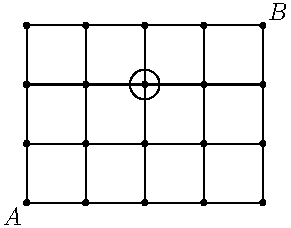
\includegraphics{yip-1-2}
  \]
\end{problem}
\begin{solution*}
  This problem is only slightly more complicated than its predecessor. We
  say slightly because thinking of the circled point as another point \(C\)
  and thinking of paths from \(A\) to \(B\) passing to \(C\) as joining
  paths from \(A\) to \(C\) and paths from \(C\) to \(D\), we have
  \(\binom{4}{2,2}\) ways to get from \(A\) to \(C\) and \(\binom{3}{2,1}\)
  ways to get from \(C\) to \(B\). Thus, we have
  \[
    \binom{4}{2,2}\binom{3}{2,1}
  \]
  paths from \(A\) to \(B\) passing through \(C\).
\end{solution*}

\begin{problem}[Ross, \S 1, \# 33]
  We have \(\$ 20,\!000\) that must be invested among \(4\) possible
  opportunities. Each investment must be integral in units of \(\$1000\),
  and there are minimal investment that need to be made if one is to invest
  these opportunities. The minimal investments are \(\$2000\), \(\$2000\),
  \(\$3000\), and \(\$4000\). How many different investment strategies are
  available if
  \begin{alphlist}
  \item an investment must be made in each opportunity?
  \item investments must be made in at least \(3\) of the \(4\)
    opportunities?
  \end{alphlist}
\end{problem}
\begin{solution*}
  Let us first cut the complexity of the problem by changing translating
  from dollars (\(\$\)) to units (\(1\) unit is \(\$1000\)). Thus, we have
  \(20\) units and we want to distribute them in integers between the \(4\)
  opportunities which require minimal investments of \(2\), \(2\), \(3\),
  and \(4\) units.
  \\\\
  For part (a), if we are to invest in each opportunity we are forced to
  give up \(2+2+3+4=11\) units and consequently are left with \(9\) units
  to distribute between the four opportunities. We can distribute \(9\)
  units between \(4\) opportunities in the total number of integer
  solutions to the linear equation \(x_1+x_2+x_3+x_4=9\) ways. The answer
  to that latter part is given by the solution to the stars and bars
  problem which in this case is
  \[
    \binom{9-1}{4-1}.
  \]
  \\\\
  For part (b), we have taken care of the case ``investments must be made
  in more that \(3\) of the \(4\) opportunities'' in part (a). Hence, we
  need only worry about the case ``investments must be made in exactly
  \(3\) of the \(4\) opportunities.'' Since our unit total will change
  depending on which \(3\) opportunities we choose, we must consider these
  \(\binom{4}{3}=4\) cases one by one.

  First, let us consider the case in which we choose the \(2\)-\(3\)-\(4\)
  opportunities. After the initial investment we have \(20-4-3-2=11\) units
  left over giving us
  \[
    \binom{11-1}{3-1}
  \]
  different distributions of our remaining units among the \(3\)
  opportunities. We double this for the case in which we choose the other
  \(2\) unit opportunity.

  Next we consider the \(2\)-\(2\)-\(3\) investment. If we go the
  \(2\)-\(2\)-\(3\) route, we have \(20-3-2-2=13\) units left over after
  the initial investment and
  \[
    \binom{13-1}{3-1}
  \]
  distributions of our units.

  Lastly, for the \(2\)-\(2\)-\(4\) route, we have \(20-2-2-4=12\) units
  left over after the initial investment giving us
  \[
    \binom{12-1}{3-1}
  \]
  distributions of our units.

  Therefore, there are
  \[
    2\binom{11-1}{3-1}
    +\binom{13-1}{3-1}
    +\binom{12-1}{3-1}
    +\binom{9-1}{4-1}
  \]
  ways of investing in at least \(3\) of the \(4\) opportunities.
\end{solution*}

\subsubsection{Theoretical exercises}
\begin{problem}[Ross, \S 1, \# 5]
  Determine the number of vectors \((x_1,\dotsc,x_n)\) such that each
  \(x_k\) is either \(0\) or \(1\) and
  \[
    \sum_{k=1}^n x_k\geq l.
  \]
\end{problem}
\begin{solution*}
  An implicit assumption must be that \(n\geq l\) for otherwise
  \((1,\dotsc,1)\) would not satisfy \(\sum_{k=1}^n x_k\geq l\). We
  henceforth assume \(n\geq l\).

  For a vector \((x_1,\dotsc,x_n)\) to satisfy
  \[
    \sum_{k=1}^n x_k\geq l
  \]
  at least \(l\) of the \(x_k\) must be \(1\). We can distribute these
  \(l\) \(1\)s between \(x_n\) in
  \[
    \binom{n+l-1}{l-1}
  \]
  by the stars and bars problem.
\end{solution*}

\begin{problem}[Ross, \S 1, \# 6]
  How many vectors \(x_1,\dotsc,x_k\) are there for which each \(x_k\) is a
  positive integer such that \(1\leq x_k\leq n\) and
  \(x_1<x_2<\dotsb<x_n\)?
\end{problem}
\begin{solution*}
\end{solution*}

\begin{problem}[Ross, \S 1, \# 8]
  Prove that
  \[
    \binom{n+m}{r}=%
    \binom{n}{0}\binom{m}{r}+\binom{n}{1}\binom{m}{r-1}%
    +\dotsb+\binom{n}{r}\binom{m}{0}.
  \]
\end{problem}
\begin{solution*}
\end{solution*}

\begin{problem}[Ross, \S 1, \# 9]
  Use Theoretical Exercise 8 to prove that
  \[
    \binom{2}{n}=\sum_{k=0}^n\binom{n}{k}^2.
  \]
\end{problem}
\begin{solution*}
\end{solution*}

\begin{problem}[Ross, \S 1, \# 12]
  Consider the following combinatorial identity:
  \[
    \sum_{k=1}^n k\binom{n}{k}=n2^{n-1}.
  \]
  \begin{alphlist}
  \item Present a combinatorial argument for this identity by considering
    the set of \(n\) people and determining, in two ways, the number of
    possible selections of a committee of any size and a chairperson for
    the committee.

    \noindent\emph{Hint:}
    \begin{enumerate}[label=(\roman*)]
    \item How many possible elections are there of a committee of size
      \(k\) and its chairperson?
    \item How many possible selections are there of a chairperson and the
      other committee members?
    \end{enumerate}
  \item Verify the following identity for \(n=1,2,3,4,5\):
    \[
      \sum_{k=1}^n \binom{n}{k}k^2=2^{n-2}n(n+1).
    \]
    For a combinatorial proof of the preceding, consider the set of \(n\)
    people and argue that both sides of the identity represent the number
    of different selections of a committee, its chairperson, and its
    secretary (possibly the same as the chairperson).

    \noindent\emph{Hint:}
    \begin{enumerate}[label=(\roman*)]
    \item How many different selection result in the committee containing
      exactly \(k\) people?
    \item How many different selections are there in which the chairperson
      and the secretary are the same? (Answer: \(n2^{n-1}\).)
    \item How many different selections result in a chairperson and the
      secretary being different?
    \end{enumerate}
  \item Now argue that
    \[
      \sum_{k=1}^n\binom{n}{k}k^3=2^{n-3}n^2(n+3).
    \]
  \end{alphlist}
\end{problem}
\begin{solution*}
\end{solution*}

\begin{problem}[Ross, \S 1, \# 23]
  Determine the number of vectors \((x_1,\dotsc,x_n)\) of \(n\) variables
  such that each \(x_k\) is a nonnegative integer and
  \[
    \sum_{k=1}^n x_k\leq l.
  \]
\end{problem}
\begin{solution*}
\end{solution*}

\subsubsection{Problems}
\begin{problem}[Ross, \S 2, \# 25]
  A pair of dice is rolled until a sum of either \(5\) or \(7\)
  appears. Find the probability that a \(5\) occurs first.

  \noindent\emph{Hint:} Let \(E_n\)
  denote the event that a \(5\) occurs on the \(n\)\textsup{th} roll and no
  \(5\) or \(7\) occurs on the first \(n-1\) rolls. Compute \(P(E_n)\) and
  argue that \(\sum_{n=1}^\infty P(E_n)\) is the desired probability.
\end{problem}
\begin{solution*}
\end{solution*}

\begin{problem}[Ross, \S 2, \# 29]
  An urn contains \(n\) white and \(m\) black balls, where \(n\) and \(m\)
  are positive numbers.
  \begin{alphlist}
  \item If two balls are randomly withdrawn, what is the probability that
    they are the same color?
  \item If a ball is randomly withdrawn and then replaced before the second
    one is drawn, what is the probability that the withdrawn balls are the
    same color?
  \item Show that the probability in part (b) is always larger than the one
    in part (a).
  \end{alphlist}
  \end{problem}
\begin{solution*}
\end{solution*}

\begin{problem}[Ross, \S 2, \# 35]
  Seven balls are randomly withdrawn from an urn that contains \(12\) red,
  \(16\) blue, and \(18\) green balls. Find the probability that
  \begin{alphlist}
  \item \(3\) red, \(2\) blue, and \(2\) green balls are withdrawn;
  \item at least \(2\) red balls are withdrawn;
  \item all withdrawn balls are the same color;
  \item either exactly \(3\) red balls or exactly \(3\) blue balls are
    withdrawn.
  \end{alphlist}
\end{problem}
\begin{solution*}
\end{solution*}

\begin{problem}[Ross, \S 2, \# 44]
  Five people, designated as \(A,B,C,D,E\), are arranged in linear
  order. Assuming that each possible order is equally likely, what is the
  probability that
  \begin{alphlist}
  \item there is exactly one person between \(A\) and \(B\)?
  \item there are exactly two people between \(A\) and \(B\)?
  \item there are three people between \(A\) and \(B\)?
  \end{alphlist}
\end{problem}
\begin{solution*}
\end{solution*}

\begin{problem}[Ross, \S 2, \# 49]
  A group of \(6\) men and \(6\) women is randomly divided into \(2\)
  groups of size \(6\) each. What is the probability that both groups will
  have the same number of men?
\end{problem}
\begin{solution*}
\end{solution*}

\subsubsection{Theoretical exercises}
\begin{problem}[Ross, \S 2, \# 5]
  For any sequence of events \(E_1,E_2,\dotsc\), define a new sequence
  \(F_1,F_2,\dotsc\), of disjoint events (that is, events such that
  \(F_j\cap F_k=\emptyset\) whenever \(j\neq k\)) such that for all \(n\geq
  1\),
  \[
    \bigcup_{k=1}^n F_k=\bigcup_{k=1}^n E_k.
  \]
\end{problem}
\begin{solution*}
\end{solution*}

\begin{problem}[Ross, \S 2, \# 14]
  Prove Proposition 4.4 by mathematical induction.
\end{problem}
\begin{solution*}
  Proposition 4.4 is called the inclusion-exclusion identity (or
  inclusion-exclusion principle which the author prefers to use).
  \begin{proposition*}[Inclusion-exclusion identity]
    \[
      \begin{split}
        P(E_1\cup E_2\cup\dotsb\cup E_n)
        =\sum_{k=1}^n P(E_k)&-\sum_{k_1<k_2} P(E_{k_1}\cap E_{k_2})\\
        &+\dotsb+(-1)^{r+1}\sum_{k_1<k_2<\dotsb<k_r}
        P(E_{k_1}\cap\dotsb\cap E_{k_r})\\
        &+\dotsb+(-1)^{n+1}P(E_1\cap\dotsb\cap E_n).
      \end{split}
    \]
    The summation
    \(\sum_{k_1<k_2<\dotsb<k_r}P(E_{k_1}\cap\dotsb\cap E_{k_r})\) is taken
    over all the \(\binom{n}{r}\) possible subsets of size \(r\) of the set
    \(\{1,\dotsc,n\}\).
  \end{proposition*}
\end{solution*}

\begin{problem}[Ross, \S 2, \# 19]
  An urn contains \(n\) red and \(m\) blue balls. They are withdrawn one at
  a time until a total of \(r\), \(r\leq n\), red balls have been
  withdrawn. Find the probability that a total of \(k\) balls are
  withdrawn.

  \noindent\emph{Hint:} A total of \(k\) balls will be withdrawn if there are \(r-1\)
  red balls in the first \(k-1\) withdrawals and the \(k\)\textsup{th}
  withdrawal is a red ball.
\end{problem}
\begin{solution*}
\end{solution*}

%%% Local Variables:
%%% mode: latex
%%% TeX-master: "../MA519-HW-ALL"
%%% End:
%
\begin{problem}[Handout 2, \# 5]
  Four men throw their watches into the sea, and the sea brings each man
  one watch back at random. What is the probability that at least one man
  gets his own watch back?
\end{problem}
\begin{solution}
  The sample space \(\Omega\) is in correspondence with \(S_4\) the set of
  bijections from the set \(\{1,\dotsc,4\}\) to itself and therefore
  \begin{equation}
    \label{eq:2-1}
    \#\Omega=\# S_4=4!=24.
  \end{equation}
  Let \(A\) denote the event that at least one man gets his own watch
  back. This is a case where it is easier find the probability of the
  complement of \(A\), i.e., the event \(\Omega\setminus A\) that no man
  gets his own watch back.

  Let \(A_i\) denote the event that the \(i\)-th man does not get his own
  watch back.
\end{solution}
\newpage

\begin{problem}[Handout 2, \#7]
  Calculate the probability that in Bridge, the hand of at least one player
  is void in a particular suit.
\end{problem}
\begin{solution}

(I read this as being equivalent to ``Calculate the probability that in a game of Bridge, some player has drawn no hearts.'')

First, note that the number of possible Bridge hands for all 4 players is 

\[
\binom{52}{13} \cdot \binom{39}{13} \cdot \binom{26}{13} \cdot \binom{52}{13}
\]

\end{solution}
\newpage

\begin{problem}[Handout 2, \# 12]
  If \(n\) balls are placed at random into \(n\) cells, find the
  probability that exactly \(1\) cell remains empty.
\end{problem}
\begin{solution}
Let $n$ balls be placed at random into $n$ cells. (As was pointed out in the feedback, we will assume that these $n$ balls are distinct.)

There are $n^n$ ways to do this.

There are

\[
\binom{n}{1} \cdot \binom{n}{2} \cdot \binom{n-1}{1} \cdot (n-2)!
\]

ways to put $n$ balls into $n$ slots with exactly one remaining empty (we pick $1$ of our $n$ slots to be empty, we pick $2$ of our $n$ balls to share a slot, we pick one of our remaining $n-1$ slots for those $2$ balls to go into, we fill the rest with one ball each.)

Thus, the probability that exactly $1$ cell remains empty is

\begin{align*}
\frac{\binom{n}{1} \cdot \binom{n}{2} \cdot \binom{n-1}{1} \cdot (n-2)!}{n^n} &= \frac{n \cdot \binom{n}{2} \cdot (n-1) \cdot (n-2)!}{n^n} \\
&= \frac{n! \cdot \frac{n-1}{2}}{n^n} \\
\end{align*}
\end{solution}
\newpage


\begin{problem}[Handout 2, \# 13]
  \emph{Spread of rumors.} In a town of \(n+1\) inhabitants, a person tells
  a rumor to a second person, who in turn repeats it to a third person,
  etc. At each step the recipient of the rumor is chosen at random from the
  \(n\) people available. Find the probability that the rumor told \(r\)
  times without:
  \begin{enumerate}[label=(\alph*),noitemsep]
  \item returning to the originator,
  \item being repeated to any person.
  \end{enumerate}
  Do the same problem when at each step the rumor told by one person to a
  gathering of \(N\) randomly chosen people. (The first question is the
  special case \(N=1\)).
\end{problem}
\begin{solution}

\end{solution}
\newpage

\begin{problem}[Handout 2, \# 14]
  \emph{A family problem.} In a certain family four girls take turns at
  washing dishes. Out of a total of four breakages, three were caused by
  the youngest girl, and she was thereafter called clumsy. Was she
  justified in attributing the frequency of breakages to chance? Discuss
  the connection with random placement of balls.
\end{problem}
\begin{solution}
Assume that it is equally likely that each girl breaks a dish.

Four girls are 
\end{solution}
\newpage

\begin{problem}[Handout 2, \# 15]
  A car is parked among \(N\) cars in a row, not at either end. On his
  return the owner finds exactly \(r\) of the \(N\) places still
  occupied. What is the probability that both neighboring places are empty?
\end{problem}
\begin{solution}

\end{solution}
\newpage

\begin{problem}[Handout 2, \# 16]
  Find the probability that in a random arrangement of \(52\) bridge card
  no two aces are adjacent.
\end{problem}
\begin{solution}

\end{solution}
\newpage

\begin{problem}[Handout 2, \# 17]
  Suppose \(P(A)=3/4\), and \(P(B)=1/3\).

  Prove that \(P(A\cap B)\geq 1/12\). Can it be equal to \(1/12\)?
\end{problem}
\begin{solution}

\end{solution}
\newpage

\begin{problem}[Handout 2, \# 18]
  Suppose you have infinitely many events \(A_1,A_2,\dotsc\), and each one
  is sure to occur, i.e., \(P(A_i)=1\) for any \(i\).
  \\\\
  Prove that \(P\bigl(\bigcap_{i=1}^n A_i\bigr)=1\).
\end{problem}
\begin{solution}

\end{solution}
\newpage

\begin{problem}[Handout 2, \# 19]
  There are \(n\) blue, \(n\) green, \(n\) red, and \(n\) white balls in an
  urn. Four balls are drawn from the urn with replacement. Find the
  probability that there are balls of at least three different colors among
  the four drawn.
\end{problem}
\begin{solution}
Each ball has an equal probability of being drawn on each draw. That is, each (ordered) set of 4 draws is equally likely to occur.

There are $4^4$ ways to draw $4$ balls.

There are $4!$ ways to draw one ball of each color.

There are $4 \cdot 3 \cdot \binom{4}{2} \cdot 2!$ ways to draw 4 balls, missing exactly one color (pick a color to be missed, pick a color to be drawn twice, pick two draws for that color to be drawn on, rearrange the other two colors into the other two draws.)

Thus, the probability of having at least three different colors being drawn among those four is

\begin{align*}
\frac{4! + 4 \cdot 3 \cdot \binom{4}{2} \cdot 2!}{4^4} &= \frac{3!+6 \cdot \frac{4!}{2!2!}}{4^3} \\
&= \frac{6+36}{4^3}\\
&\cong 0.65625\\
\end{align*}
\end{solution}

%%% Local Variables:
%%% mode: latex
%%% TeX-master: "../MA519-Current-HW"
%%% End:
%
\begin{problem}[Handout 3, \# 3]
  \(n\) sticks are broken into one short and one long part. The \(2n\)
  parts are then randomly paired up to form \(n\) new sticks. Find the
  probability that
  \begin{enumerate}[label=(\alph*),noitemsep]
  \item the parts are joined in their original order, i.e., the new sticks
    are the same as the old sticks;
  \item each long part is paired up with a short part.
  \end{enumerate}
\end{problem}
\begin{solution}
  For part (a), let \(\Omega\) denote the sample space. Then, there are
  \(2n(2n-1)\) ways to pair the sticks together. Let \(A\) denote the event
  that two parts are joined in their original order. We have \(2n\) ways to
  chose one end and, once we have made that choice, only \(1\) way to chose
  the complementary end. Thus,
  \[
    P(A)=\frac{2n\cdot 1}{2n(2n-1)}=\frac{1}{2n-1}.
  \]

  For part (b), the sample space \(\Omega\) remains as before. Let \(A\)
  denote the event that each long part is joined with a short part. Then we
  have
\end{solution}
\newpage

\begin{problem}[Handout 3, \# 5]
  In a town, there are \(3\) plumbers. On a certain day, \(4\) residents
  need a plumber and they each call one plumber at random.
  
  a) What is the probability that all the calls go to one plumber (not necessarily a specific one)?
  
  b) What is the expected value of the number of plumbers who get a call?
\end{problem}
\begin{solution}

Label the plumbers as $a$, $b$, and $c$. Let $A$ be the event that plumber $a$ gets every call, let $B$ be the event that plumber $b$ gets every call, and let $C$ be the event that plumber $c$ gets every call.

For a): Let $A$ be the event that plumber $a$ gets every call, let $B$ be the event that plumber $b$ gets every call, and let $C$ be the event that plumber $c$ gets every call.
Then $P(A) = P(B) = P(C) = \frac{1}{3^4}$. (The probability of plumber $a$ getting called by the first resident is $1/3$. The residents call independently, the probability that all $4$ residents call him is $(1/3)^4$). Because all events are disjoint, $P(A \cup B \cup C) = \frac{1}{3^4} + \frac{1}{3^4} + \frac{1}{3^4}$.

That is, the probability that some plumber gets every call is $\frac{1}{3^3} = \frac{1}{27} \cong 0.037$.

For b): Let $\scrX$ be the number of plumbers who get called.

As above, 

\[
P(\scrX = 1) = \frac{1}{27}.
\]

Similar to the above,

\[
P(\scrX = 2) = 3\left(\left(\frac{2}{3}\right)^4 - \frac{2}{3^4} \right)
\]

(The probability of a resident calling either plumber $a$ or plumber $b$ is $(2/3)$. The probability of every resident calling one of plumber $a$ or $b$ is $(2/3)^4$. The probability that plumber $a$ was the only plumber called is $(1/3)^4$. The probability that plumber $b$ was the only plumber called is $(1/3)^4$. Thus, the probability that plumber $a$ and plumber $b$ have both been called without calling plumber $c$ is $(2/3)^4 - 2/3^4$. The probability that two plumbers have been called is the sum of the probabilities that exactly plumbers $a$ and $b$ have been called, exactly plumbers $b$ and $c$ have been called, and exactly plumbers $a$ and $c$ have been called; that is, it is as given above.)

Last,

\[
P(\scrX = 3) = 1-P(\scrX = 1)-P(\scrX = 2)
\]

So that

\begin{align*}
E(\scrX) &= P(\scrX=1) + 2P(\scrX=2) + 3P(\scrX = 3) \\
&= \frac{1}{27} + 6\left(\left(\frac{2}{3}\right)^4 - \frac{2}{3^4} \right) + 3\left(1-\frac{1}{27} -  3\left(\left(\frac{2}{3}\right)^4 - \frac{2}{3^4} \right)\right) \\
&= \frac{1}{27} + 6\frac{2^4}{3^4} - \frac{12}{3^4} + 3-\frac{1}{9} -  9\left(\left(\frac{2}{3}\right)^4 - \frac{2}{3^4} \right)\\
&= \frac{1}{27} + 6\frac{16}{81} - \frac{12}{81} + 3-\frac{1}{9} -  \frac{16}{9} - \frac{2}{9}\\
&= \frac{53}{27}\\
&\cong 1.962
\end{align*}

That is, the expected number of plumbers that get called is $\frac{53}{27}$, which is slightly less than two.

\end{solution}
\newpage

\begin{problem}[Handout 4, \# 7]
  \emph{(Polygraphs).} Polygraphs are routinely administered to job
  applicants for sensitive government positions. Suppose someone actually
  lying fails the polygraph \(90\%\) of the time. But someone telling the
  truth also fails the polygraph \(15\%\) of the time. If a polygraph
  indicates that an applicant is lying, what is the probability that he is
  in fact telling the truth? Assume a general prior probability \(p\) that
  the person is telling the truth.
\end{problem}
\begin{solution}

Let $TRUTH$ denote the event that the person is telling the truth. Set $P(TRUTH) = p$.

Let $FAIL$ denote the event that the person fails the polygraph. Let $LIE$ denote the event that the person has lied. Then $P(FAIL | LIE) = 0.9$, and $P(FAIL | TRUTH) = 0.15$.

By Bayes' Theorem,

\[
P(TRUTH | FAIL) = \frac{P(FAIL | TRUTH) \cdot P(TRUTH)}{P(FAIL | TRUTH) \cdot P(TRUTH) + P(FAIL | LIE) \cdot P(LIE)}
\]

which reduces to

\[
P(TRUTH | FAIL) = \frac{0.15p}{0.15p + 0.9 - 0.9p} = \frac{0.15p}{0.9 - 0.75p}
\]

\end{solution}
\newpage

\begin{problem}[Handout 4, \# 8]
  In a bolt factory machines \(A\), \(B\), \(C\) manufacture, respectively,
  \(25\), \(35\), and \(40\) per cent of the total. Of their output \(5\),
  \(4\), and \(2\) per cent are defective bolts. A bolt is drawn at random
  from the produce and is found defective. What are the probabilities that
  it was manufactured by machines \(A\), \(B\), \(C\)?
\end{problem}
\begin{solution}

Let $DEF$ denote the event in which the random bolt we have drawn was defective. Let $A$, $B$, and $C$ denote the events in which we have drawn our bolts from machines $A$, $B$, and $C$ (respectively).

Then

\begin{align*}
P(DEF | A) &= 0.05 \\
P(DEF | B) &= 0.04 \\
P(DEF | C) &= 0.02 \\
P(A) &= 0.25 \\
P(B) &= 0.35 \\
P(C) &= 0.4 \\
\end{align*}

Which means that, by Bayes' Theorem,

\begin{align*}
P(A | DEF) &= \frac{P(DEF | A) \cdot P(A)}{P(DEF | A)P(A) + P(DEF |B) P(B) + P(DEF|C)P(C)} \\
&= \frac{0.05 \cdot 0.25}{0.05 \cdot 0.25 + 0.04 \cdot 0.35 + 0.02 \cdot 0.4 } \\
&= \frac{0.0125}{0.0125 + 0.014 + 0.008} \\
&= \frac{0.0125}{0.0345} \\
&\cong 0.36 \\
\end{align*}

\begin{align*}
P(B | DEF) &= \frac{0.014}{0.0125 + 0.014 + 0.008} \\
&= \frac{0.014}{0.0345} \\
&\cong 0.41 \\
\end{align*}

\begin{align*}
P(C | DEF) &= \frac{0.008}{0.0125 + 0.014 + 0.008} \\
&= \frac{0.008}{0.0345} \\
&\cong 0.23 \\
\end{align*}

That is, there's about a $36$ percent chance that our defective bolt came from $A$, a $41$ percent chance it came from $B$, and a $23$ percent chance it came from $C$.

\end{solution}
\newpage

\begin{problem}[Handout 4, \# 9]
  Suppose that \(5\) men out of \(100\) and \(25\) women out of
  \(\num{10000}\) are colorblind. A colorblind person is chosen at
  random. What is the probability of his being male? (Assume males and
  females to be in equal numbers.)
\end{problem}
\begin{solution}

Let $CB$ be the event that a randomly chosen person is color blind. Let $M$ be the event that the randomly chosen person was male, and let $F$ be the event that the randomly chosen person was female.

Then

\begin{align*}
P(CB | M) &= 0.05 \\
P(CB | F) &= 0.0025
\end{align*}

So, by Bayes' Theorem,

\begin{align*}
P(M | CB) &= \frac{P(CB|M)P(M)}{P(CB|M)P(M) + P(CB|F)P(F)}\\
&= \frac{0.05}{0.05+0.0025}\\
&= \frac{0.05}{0.0525}\\
&\cong 0.95
\end{align*}

That is, there is about a $95$ percent chance that the randomly chosen color blind person was male.

\end{solution}
\newpage

\begin{problem}[Handout 4, \# 10]
  \emph{Bridge.} In a bridge party West has no ace. What probability should
  he attribute to the event of his partner having
  \begin{enumerate}[label=(\alph*),noitemsep]
  \item no ace,
  \item two or more aces?
  \end{enumerate}
  Verify the result by a direct argument.
\end{problem}
\begin{solution}

\end{solution}
\newpage

\begin{problem}[Handout 4, \# 12]
  A true-false question will be posed to a couple on a game show. The
  husband and the wife each has a probability \(p\) of picking the correct
  answer. Should they decide to let one of the answer the question, or
  decide that they will give the common answer if they agree and toss a
  coin to pick the answer if they disagree?
\end{problem}
\begin{solution}

The probability that the couple wins if they let one of them answer the question is $p$ (that is, it is the probability that that person gets it right.)

The probability that the couple wins if they give a common answer if they agree and toss a coin to pick the answer if they disagree is the sum of the probabilities that they agree on the correct answer and the probability that they guess differently and then win on the coin flip.

The probability that they agree on the correct answer is $p^2$.

The probability that they guess differently is $2(1-p)p$; that is, this is the probability that the husband is wrong and the wife is right plus the probability that the wife is wrong and the husband is right. The probability that they win, given that they've guessed differently, is $1/2$. So, the probability that they win because of the coin flip after they guess differently is $(1-p)p$.

So, the probability that they win in this fashion is $p^2 + (1-p)p = p$.

That is, from the perspective of the game, it does not matter which course of action they take. They should do whichever thing is most likely to make them the least mad at each other if they lose.

\end{solution}
\newpage

\begin{problem}[Handout 4, \# 13]
  An urn containing \(5\) balls has been filled up by taking \(5\) balls at
  random from a second urn which originally had \(5\) black and \(5\) white
  balls. A ball is chosen at random from the first urn and is fonud to be
  black. What is the probability of drawing a white ball if a second ball
  is chosen from among the remaining \(4\) balls in the first urn?
\end{problem}
\begin{solution}

\end{solution}
\newpage

\begin{problem}[Handout 4, \# 15]
  Events \(A\), \(B\), \(C\) have probabilities \(p_1\), \(p_2\),
  \(p_3\). Given that exactly two of the three events occured, the
  probability that \(C\) occured is greater than \(1/2\) if and only if
  ... (write down the necessary and sufficient condition).
\end{problem}
\begin{solution}

\end{solution}
\newpage

\begin{problem}[Handout 5, \# 1]
  There are five coins on a desk: \(2\) are double-headed, \(2\) are
  double-tailed, and \(1\) is a normal coin.
  \\\\
  One of the coins is selected at random and tossed. It shows heads.
  \\\\
  What is the probability that the other side of this coin is a tail?
\end{problem}
\begin{solution}

\end{solution}
\newpage

\begin{problem}[Handout 5, \# 2]
  \emph{(Genetic testing).} There is a \(50\)-\(50\) chance that the Queen
  carries the gene for hemophilia. If she does, then each Prince has a
  \(50\)-\(50\) chance of carrying it. Three Princesses were recently
  tested and found to be non-carriers. Find the following probabilities:
  \begin{enumerate}[label=(\alph*),noitemsep]
  \item that the Queen is a carrier;
  \item that the fourth Princess is a carrier.
  \end{enumerate}
\end{problem}
\begin{solution}

\end{solution}
\newpage

\begin{problem}[Handout 5, \# 4]
  \emph{(Is Johnny in Jail).} Johnny and you are roommates. You are a
  terrific student and spend Friday evenings drowned in books. Johnny
  always goes out on Friday evenings. \(40\%\) of the times, he goes out
  with his girlfriend, and \(60\%\) of the times he goes to a bar. If he
  goes out with his girlfriend, \(30\%\) of the times he is just too lazy
  to come back and spends the night at hers. If he goes to a bar, \(40\%\)
  of the times he gets mad at the person sitting on his right, beats him
  up, and goes to jail.
  \\\\
  On one Saturday morning, you wake up to see Johnny is missing. Where is
  Johnny?
\end{problem}
\begin{solution}

\end{solution}

%%% Local Variables:
%%% mode: latex
%%% TeX-master: "../MA519-Current-HW"
%%% End:
%
\begin{problem}[Ross, \S 4, \# 4]
\end{problem}
\begin{solution*}
\end{solution*}

\begin{problem}[Ross, \S 4, \# 21]
\end{problem}
\begin{solution*}
\end{solution*}

\begin{problem}[Ross, \S 4, \# 22]
\end{problem}
\begin{solution*}
\end{solution*}

\begin{problem}[Ross, \S 4, \# 36]
\end{problem}
\begin{solution*}
\end{solution*}

\begin{problem}[Ross, \S 4, \# 37]
\end{problem}
\begin{solution*}
\end{solution*}

\begin{problem}[Ross, \S 4, \# 42]
\end{problem}
\begin{solution*}
\end{solution*}

\begin{problem}[Ross, \S 4, \# 43]
\end{problem}
\begin{solution*}
\end{solution*}

\begin{problem}[Ross, \S 4, \# 4]
\end{problem}
\begin{solution*}
\end{solution*}

\begin{problem}[Ross, \S 4, \# 5]
\end{problem}
\begin{solution*}
\end{solution*}

\begin{problem}[Ross, \S 4, \# 10]
\end{problem}
\begin{solution*}
\end{solution*}

\begin{problem}[Ross, \S 4, \# 13]
\end{problem}
\begin{solution*}
\end{solution*}

\begin{problem}[Ross, \S 4, \# 14]
\end{problem}
\begin{solution*}
\end{solution*}

\begin{problem}[Ross, \S 4, \# 18]
\end{problem}
\begin{solution*}
\end{solution*}

\begin{problem}[Ross, \S 4, \# 25]
\end{problem}
\begin{solution*}
\end{solution*}

\begin{problem}[Ross, \S 4, \# 27]
\end{problem}
\begin{solution*}
\end{solution*}

\begin{problem}[Ross, \S 4, \# 30]
\end{problem}
\begin{solution*}
\end{solution*}

\begin{problem}[Ross, \S 4, \# 32]
\end{problem}
\begin{solution*}
\end{solution*}

\begin{problem}[Ross, \S 4, \# 34]
\end{problem}
\begin{solution*}
\end{solution*}

%%% Local Variables:
%%% mode: latex
%%% TeX-master: "../MA519-HW-ALL"
%%% End:
%
% \subsection{Homework 5}
Ross, 9th edition:
Chapter 7:
Problems: #16, 25, 26, 38, 40, 70, 71, 72;
Theoretical Exercises: #10, 17, 38, 41
Chapter 8:
Problems: #1, 2, 3, 4, 9, 13;
Theoretical Exercises: #6, 7.

%%% Local Variables:
%%% mode: latex
%%% TeX-master: "../MA519-HW-ALL"
%%% End:
%
% \subsection{Homework 6}
\subsubsection{Problems}
\begin{problem}[Ross, \S 6, \# 1]
\end{problem}
\begin{solution*}
\end{solution*}

\begin{problem}[Ross, \S 6, \# 8]
\end{problem}
\begin{solution*}
\end{solution*}

\begin{problem}[Ross, \S 6, \# 9]
\end{problem}
\begin{solution*}
\end{solution*}

\begin{problem}[Ross, \S 6, \# 17]
\end{problem}
\begin{solution*}
\end{solution*}

\begin{problem}[Ross, \S 6, \# 19]
\end{problem}
\begin{solution*}
\end{solution*}

\begin{problem}[Ross, \S 6, \# 23]
\end{problem}
\begin{solution*}
\end{solution*}

\begin{problem}[Ross, \S 6, \# 27]
\end{problem}
\begin{solution*}
\end{solution*}

\begin{problem}[Ross, \S 6, \# 40]
\end{problem}
\begin{solution*}
\end{solution*}

\begin{problem}[Ross, \S 6, \# 41]
\end{problem}
\begin{solution*}
\end{solution*}

\begin{problem}[Ross, \S 6, \# 42]
\end{problem}
\begin{solution*}
\end{solution*}

\begin{problem}[Ross, \S 6, \# 43]
\end{problem}
\begin{solution*}
\end{solution*}

\begin{problem}[Ross, \S 6, \# 54]
\end{problem}
\begin{solution*}
\end{solution*}

\begin{problem}[Ross, \S 6, \# 55]
\end{problem}
\begin{solution*}
\end{solution*}

\begin{problem}[Ross, \S 6, \# 56]
\end{problem}
\begin{solution*}
\end{solution*}

\begin{problem}[Ross, \S 6, \# 57]
\end{problem}
\begin{solution*}
\end{solution*}

%%% Local Variables:
%%% mode: latex
%%% TeX-master: "../MA519-HW-ALL"
%%% End:
%
% \begin{problem}[Handout 10, \# 4]
  \emph{(Poisson Approximation.)} One hundred people will each toss a fair
  coin \(200\) times. Approximate the probability that at least \(10\) of
  the \(100\) people would each have obtained exactly \(100\) heads and
  \(100\) tails.
\end{problem}
\begin{solution}
  Let \(X\) denote the number of people who obtain exactly \(100\) heads
  and (consequently) \(100\) tails. First, we compute the probability that
  any one given person obtains exactly \(100\) heads. There are \(2^{200}\)
  possible outcomes for \(200\) tosses of a fair coin, and
  \(\binom{200}{100}\) possible ways of obtaining exactly \(100\)
  heads. Thus, the probability that any one person obtains exactly \(100\)
  head in \(200\) tosses of a fair coin is
  \[
    p=\frac{\binom{200}{100}}{2^{200}}\approx\num{0.05634847900925642}.
  \]

  Now, assuming \(X\sim\Poisson(\num{5.634847900925642})\), the
  probability that at least \(10\) of the \(100\) people have each obtained
  exactly \(100\) heads and \(100\) tails is
  \begin{align*}
    P(X\geq 10)
    &=1-P(X<10)\\
    &=1-\sum_{i=1}^9 P(X=i)\\
    &=1
      -e^{-\num{5.634847900925642}}
      \sum_{i=0}^9\frac{\num{5.634847900925642}^i}{i!}\\
    &=1-\num{0.8825634032515405}\\
    &\approx \num{0.11743659674845952}.
  \end{align*}
\end{solution}
\newpage

\begin{problem}[Handout 10, \# 5]
  \emph{(A Pretty Question.)} Suppose \(X\) is a Poisson distributed random
  variable. Can three different values of \(X\) have an equal probability?
\end{problem}
\begin{solution}
  No. Let \(X\sim\Poisson(\lambda)\). First, we show that given any two
  values \(k_1,k_2\in\bbZ_{\geq 0}\), there exists \(\lambda\) such that
  \(p(k_1)=p(k_2)\).

  Observe that for \(p(k_1)=p(k_2)\) we must have
  \begin{align*}
    e^{-\lambda}\frac{\lambda^{k_1}}{k_1!}
    &=e^{-\lambda}\frac{\lambda^{k_2}}{k_2!}\\
    \lambda^{k_1-k_2}
    &=\frac{k_1!}{k_2!}
      \intertext{this implies that, given \(k_1\) and \(k_2\),}
      (k_1-k_2)\ln\lambda&=\ln(k_1!/k_2!)\\
    \lambda(k_1,k_2)&=e^{\ln(k_1!/k_2!)/(k_1-k_2)}.
  \end{align*}
  For example, \(\lambda(3,5)\approx\num{4.472135954999579}\) and
  \[
    p(3)\approx\num{0.17028240507308132}\approx p(5).
  \]

  We now prove our original claim. Assume for a moment that \(X\) is
  continuous. We will show that the PMF \(p\) of \(X\) has at most one
  critical point. Write the PMF of \(p\) as its continuous analogue
  \[
    p(x)=P(X=x)=\frac{e^{-\lambda}\lambda^x}{\Gamma(x)}.
  \]
  Then, taking the derivative of \(p\), we have
  \begin{align*}
    p'(x)
    &=e^{-\lambda}\frac{\Gamma(x)\lambda^x\ln\lambda-\lambda^x\Gamma(x)}{\Gamma(x)^2}\\
    &=\frac{e^{-\lambda}\lambda^x}{\Gamma(x)}
      \left[\ln\lambda-\frac{\Gamma'(x)}{\Gamma(x)}\right]\\
    &=p(x)\left[\ln\lambda-\frac{\Gamma'(x)}{\Gamma(x)}\right].
  \end{align*}
  Since \(\Gamma,\Gamma'>0\) for all \(x\in\bbR_{\geq 0}\), \(p'(x)=0\) if
  and only if
  \[
    \ln\lambda=\frac{\Gamma'(x)}{\Gamma(x)}
  \]
  which happens at most once since the quotient.
\end{solution}
\newpage

\begin{problem}[Handout 10, \# 6]
  \emph{(Poisson Approximation.)} There are \(20\) couples seated at a
  rectangular table, husbands on one side and the wives on the other, in a
  random order. Using a Poisson approximation, find the probability that
  exactly two husbands are seated directly across from their wives; at
  least three are; at most three are.
\end{problem}
\begin{solution}
  Let \(X\) count the number of husbands that have been seated directly
  across from their respective wives. We approximate the probabilities that
  (i) exactly two husbands are seated directly across from their wives,
  (ii) at least three are, and (iii) at most three are, by assuming that
  \(X\sim\Poisson(\lambda)\). But first, we compute the probability \(p\)
  that exactly one husband has been seated directly across from his wife.

  There are \(20!\) arrangements for the
  couples. Fixing the husbands, there are \(20\) ways to pick the wife that
  is to be seated directly across from her husband. There remain \(19\)
  couples and we want none of these to be seated right across from each
  other. To this end, and in order to save some time, we use the formula
  for counting \emph{derangements}, which can be derived from the
  inclusion-exclusion principle,
  \begin{align*}
    !19&=19!\sum_{i=0}^n\frac{(-1)^i}{i!}\\
       &=\num{44750731559645100}.
  \end{align*}
  Thus,
  \[
    p=\frac{20(!19)}{20!}=\frac{!19}{19!}\approx\num{0.3678794411714423},
  \]
  so \(\lambda\approx\num{7.357588823428846}\).

  With this, we can proceed to approximate (i) the probability that exactly
  two husbands are seated across from their wives. This is given by
  \[
    p(2)=e^{-\num{7.357588823428846}}\frac{\num{7.357588823428846}^2}{2!}
    \approx\num{0.01726159034832215}
  \]
\end{solution}
\newpage

\begin{problem}[Handout 10, \# 7]
  \emph{(Poisson Approximation.)} There are \(5\) coins on a desk, with
  probabilities \(0.05\), \(0.1\), \(0.05\), \(0.01\), and \(0.04\) for
  heads. By using a Poisson approximation, find the probability of
  obtaining at least one head when the five coins are each tossed once.

  \noindent Is the number of heads obtained binomially distributed in this
  problem?
\end{problem}
\begin{solution}
  First, let us find the probability \(p\) that the toss of a coin randomly
  selected from the \(5\) comes up heads. This is given by
  \[
    p=\frac{0.05+0.1+0.05+0.01+0.04}{5}=0.05.
  \]
  Now, \(\lambda=0.25\) so the probability of obtaining at least one head
  is
  \[
    e^{-0.25}\sum_{i=1}^5 \frac{0.25^i}{i!}\approx\num{0.22119894311503177}.
  \]
\end{solution}
\newpage

\begin{problem}[Handout 10, \# 8]
  A book of \(500\) pages contains \(500\) misprints. Estimate the chances
  that a given page contains at least three misprints.
\end{problem}
\begin{solution}
  We approximate the distribution of \(X\) the number of misprints on a
  given page using a Poisson distribution with parameter \(\lambda=1\) the
  density of misprints throughout the book. Under these assumptions, the
  probability that a given page contains at least three misprints is given
  by
  \[
    1-e^{-1}\frac{1}{1!}-e^{-1}\frac{1}{1!}-e^{-1}\frac{1}{2!}
    \approx\num{0.08030139707139416}.
  \]
\end{solution}
\newpage

\begin{problem}[Handout 10, \# 9]
  Estimate the number of raisins which a cookie should contain on the
  average if it is desired that not more than one cookie out of a hundred
  should be without raisin.
\end{problem}
\begin{solution}
  The number of raisins in a cookie is given by a poisson distribution: let
  $X_{\la}$ be the number of raisins in a cookie that came out of a batch
  where the average number of raisins per cookie was $\lambda$. We want
  $P(X_{\lambda} = 0) \leq 0.01$. That is, we want
  \[
    \frac{\lambda^0 e^{-\lambda}}{0!} = e^{-\lambda} \leq 0.01
  \]
  which occurs for $\lambda \geq -\ln(0.01) = \ln(100) \approx 4.60517$.

  That is, we want there to be about $4.6$ raisins per cookie in order to
  guarantee that no more than one out of one hundred cookies is raisinless.
\end{solution}
\newpage

\begin{problem}[Handout 10, \# 10]
  The terms \(p(k;\lambda)\) of the Poisson distribution reach their
  maximum when \(k\) is the largest integer not exceeding \(\lambda\).
\end{problem}
\begin{solution}
  First, set $\floor{\lambda}$ equal to the largest integer not exceeding
  $\lambda$. Then we show $p(k;\lambda)$ is increasing on
  $[0,\floor{\lambda}]$ and decreasing on $[\floor{\lambda}, \infty)$; this
  suffices to show that the maximum occurs at $\floor{\lambda}$.

  Now, note that for all $k$,
  \begin{align*}
    p(k; \lambda) - p(k+1;\lambda) &= \frac{\lambda^k e^{-\lambda}}{k!} -\frac{\lambda^{k+1} e^{-\lambda}}{(k+1)!}\\
                                   &= \frac{e^{-\lambda} \lambda^k}{k!} \left( 1 -\frac{\lambda}{k+1} \right)\\
                                   &= \frac{e^{-\lambda} \lambda^k}{k!} \left( 1 -\frac{\lambda}{k+1} \right)\\
  \end{align*}
  which is positive exactly when $k < \lambda +1$ and negative exactly when
  $k \geq lambda +1$. That is, $p(k+1;\lambda)$ is larger than
  $p(k; \lambda)$ exactly when $k < \lambda +1$; that is, $p(k;\lambda)$
  increases until the largest integer not exceeding $\lambda$;
  $p(k;\lambda)$ is increasing on $[0,\floor{\lambda}$ and decreasing on
  $[\floor{\lambda},\infty)$, as desired.
\end{solution}
\newpage

\begin{problem}[Handout 10, \# 11]
  Prove
  \[
    p(0,\lambda)+\dotsb+p(n,\lambda)
    =\frac{1}{n!}\int_\lambda^\infty e^{-x}x^n\diff x.
  \]
\end{problem}
\begin{solution}
  By integration by parts, we have
  \begin{align*}
    \frac{1}{n!}\int_\lambda^\infty e^{-x}x^n\diff x
    &=\frac{1}{n!}e^{-x}x^n\Bigr|_\lambda^\infty-\frac{1}{n!}\int_\lambda^\infty
      -ne^{-x}x^{n-1}\diff x\\
    &=\frac{e^{-\lambda}\lambda^n}{n!}+\frac{1}{(n-1)!}\int_\lambda^\infty
      e^{-x}x^{n-1}\diff x\\
    &\vdotswithin{=}\\
    &=\frac{e^{-\lambda}\lambda^n}{n!}+\frac{e^{-\lambda}\lambda^{n-1}}{(n-1)!}+\dotsb+
      \frac{e^{-\lambda}\lambda^{0}}{0!}\\
    &=p(n;\lambda)+\dotsb+p(0;\lambda),
  \end{align*}
  as was to be shown.
\end{solution}
\newpage

\begin{problem}[Handout 10, \# 12]
  There is a random number \(N\) of coins in your pocket, where \(N\) has a
  Poisson distribution with mean \(\mu\). Each one is tossed once.

  \noindent Let \(X\) be the number of times a head shows.

  \noindent Find the distribution of \(X\).
\end{problem}
\begin{solution}
  First, note that $P(N=n) = \frac{e^{-\mu} \mu^n}{n!}$.  Given that there
  are $n$ coins in your pocket, let $X_n$ denote the number of heads
  shown. Then $P(X_n = m) = \binom{n}{m} \left( 0.5 \right)^n$.  So, the
  distribution of $X$ is given by
  \begin{align*}
    P(X=m) &= \sum\limits_{n=0}^\infty P(X_n = m) P(N=n) \\
           &= \sum\limits_{n=0}^\infty \binom{n}{m} \left( 0.5 \right)^n \frac{e^{-\mu} \mu^n}{n!} \\
           &= e^{-\mu} \sum\limits_{n=0}^\infty \frac{n!}{(n-m)!m!n!} (0.5 \mu)^n \\
           &= \frac{e^{-\mu}}{m!} \sum\limits_{n=0}^\infty \frac{(0.5 \mu)^n}{(n-m)!}
  \end{align*}
\end{solution}
\newpage

\begin{problem}[Handout 10, \# 14]
  Find the MGF of a general Poisson distribution, and hence prove that the
  mean and the variance of an arbitrary Poisson distribution are equal.
\end{problem}
\begin{solution}
Let $X$ be a poisson distribution with mean $\lambda$. Then

\begin{align*}
M_X(t) &= \sum\limits_{n=0}^\infty e^{tn} P(X = n) \\
&= \sum\limits_{n=0}^\infty e^{tn} \frac{e^{-\lambda} \lambda^n}{n!} \\
&= e^{-\lambda} \sum\limits_{n=0}^\infty \frac{(e^t \lambda)^n}{n!} \\
&= e^{-\lambda} e^{\lambda e^t} \\
\end{align*}

Note that $M_X'(t) = e^{-\lambda} \left(\lambda e^{\lambda e^t + t} \right)$ and $M_X''(t) = e^{-\lambda} \left(\lambda e^{\lambda e^t + t} \right) \left(\lambda e^t +1 \right)$.

Evaluating at $0$, we get that $E(X) = M_X'(0) = \lambda$ and $E(X^2) = M_X''(0) /2= \lambda$.
\end{solution}
\newpage

\begin{problem}[Handout 10, \# 17 (a)]
  \emph{(Poisson approximations.)} \(20\) couples are seated in a
  rectangular table, husbands on one side and the wives on the
  other. First, find the expected number of husbands that sit directly
  across from their wives. Then, using a Poisson approximation, find the
  probability that two do; three do; at most five do.
\end{problem}
\begin{solution}

\end{solution}

%%% Local Variables:
%%% mode: latex
%%% TeX-master: "../MA519-HW-Current"
%%% End:
%

%% Quals
%%% DasGupta
\section{Midterms, Exams, and Qualifying Exams}
\subsection{Qualifying Exams, August `99}
\begin{problem}
  The number of fish that Anirban catches on any given day has a Poisson
  distribution with mean \(20\). Due to the legendary softness of his
  heart, he sets free, on average, \(3\) out of the \(4\) fish he
  catches. Find the mean and the variance of the number of fish Anirban
  takes home on a given day.
\end{problem}
\begin{solution*}
  Let \(X\) denote the number of fish caught by Anirban on any given day
  and let \(Y\) denote the number of fish released by Anirban. Since
  Anirban releases on average three-fourths of the fish he catches, the
  number of fish he keeps is
  \[
    K\defeq X-Y=X-\tfrac{3}{4}Y=\tfrac{1}{4}X.
  \]
  Therefore,
  \[
    E(K)=\tfrac{1}{4}E(X)=\frac{20}{4}=5
  \]
  and
  \[
    \Var(K)=\left(\tfrac{1}{4}\right)^2\Var(X)=\frac{20}{16}.
  \]
\end{solution*}

\begin{problem}
  A fair die is rolled and at the same time a fair coin is tossed. This is
  done repeatedly. Find the probability that head occurs (strictly) before
  six occurs.
\end{problem}
\begin{solution*}
  Let \(X\) denote the number of tosses until a head comes up and \(Y\)
  denote the number of rolls until we roll a six. Both of these random
  variables have geometric PMFs with parameters \(\frac{1}{2}\) and
  \(\frac{1}{6}\), respectively. Then we need to find \(P(X<Y)\). Since
  \(X\) and \(Y\) are independent this value is given by the sum
  \begin{align*}
    P(X<Y)
    &=P(0<Y-X)\\
    &=\sum_{k=1}^\infty\sum_{\ell=k+1}^\infty P(X=k)P(Y=\ell)\\
    &=\sum_{k=1}^\infty\sum_{\ell=k+1}^\infty
      \left(\frac{1}{2}\right)\left(\frac{1}{2}\right)^{k-1}
      \left(\frac{1}{6}\right)\left(\frac{5}{6}\right)^{\ell-1}\\
    &=\sum_{k=1}^\infty\sum_{\ell=k+1}^\infty\\
    &=\left(\frac{1}{12}\right)
     \left[\sum_{k=0}^\infty
      \left(\frac{1}{12}\right)^{k-1}
      \right]
      \left[\sum_{\ell=0}^\infty \left(\frac{5}{6}\right)^\ell\right]\\
    &=\left(\frac{1}{12}\right)
      \left(\frac{1}{1-\frac{1}{12}}\right)
      \left(\frac{1}{1-\frac{5}{6}}\right)\\
    &=\frac{6}{11}.\qedhere
  \end{align*}
\end{solution*}

\begin{problem}
  \(X\), \(Y\) are independent random variables with a common density
  \(f(x)=\frac{\rme^{-|x|}}{2}\), \(x\in(-\infty,\infty)\). Find the
  density function of \(X+Y\).
\end{problem}
\begin{solution*}
\end{solution*}

\begin{problem}
  Let \(X_n\) denote the distance between two points chosen independently
  at random from the unit cube in \(\bbR^n\). Evaluate
  \[
    \lim_{n\to\infty}\frac{E(X_n)}{\sqrt{n}}.
  \]
\end{problem}
\begin{solution*}
\end{solution*}

\begin{problem}
  Let \(X\) be distributed as \(U[0,1]\). What is the probability that the
  digit \(5\) does not occur in the decimal expansion of \(X\)?
\end{problem}
\begin{solution*}
\end{solution*}

%%% Local Variables:
%%% mode: latex
%%% TeX-master: "../MA519-HW-ALL"
%%% End:

\subsection{Qualifying Exam, January `06}
\begin{problem}
  The birthdays of \(5\) people are known to fall in exactly \(3\) calendar
  months. What is the probability that exactly two of the \(5\) were born
  in January?
\end{problem}
\begin{solution*}
\end{solution*}

\begin{problem}
  Coupons are drawn, independently, with replacement, one at a time, from a
  set of \(10\) coupons. Find, explicitly, the expected number of draws
  \begin{enumerate}[label=(\alph*),noitemsep]
  \item until the first draw coupon is drawn again;
  \item until a duplicate occurs.
  \end{enumerate}
\end{problem}
\begin{solution*}
\end{solution*}

\begin{problem}
  Let \(N\) be a positive integer. Choose an integer at random from
  \(\{1,\dotsc,N\}\). Let \(E\) be the event that your chosen random number
  is divisible by \(3\), and divisible by at least one of \(4\) and \(6\),
  but not divisible by \(5\). Find, explicitly, \(\lim_{N\to\infty}P(E)\).
\end{problem}
\begin{solution*}
\end{solution*}

\begin{problem}
  Anirban is driving his Dodge on a highway with \(4\) lanes each way. He
  is wired to change lanes every minute on the minute. He changes with
  equal probability to either adjacent lane if there are two adjacent
  lanes, and the successive changes are mutually independent. Find,
  explicitly, the probability that after \(4\) minutes, Anirban is back to
  the lane he started from
  \begin{enumerate}[label=(\alph*),noitemsep]
  \item if he started at an outside lane;
  \item if he started at an inside lane.
  \end{enumerate}
\end{problem}
\begin{solution*}
\end{solution*}

\begin{problem}
  Burgess is going to Moose Pass, Alaska. He is driving his Dodge. He puts
  his car on cruise control at \(\SI{70}{\mph}\). Gas stations are located
  every \(30\) miles, starting from his home. His car runs out of gas at a
  time distributed as an exponential with mean \(4\) hours. When that
  happens, he gets out, takes his bik out of his trunk, and bikes to the
  next gas station say \(M\), at \(\SI{10}{\mph}\). Let the time elapsed
  between when Burgess starts his trip and when he arrives at the gas
  station \(M\) be \(T\). Find \(E(T)\).
\end{problem}
\begin{solution*}
\end{solution*}

\begin{problem}
  A fair coin is tossed \(n\) times. Suppose \(X\) heads are
  obtained. Given \(X=x\), let \(Y\) be generated according to the Poisson
  distribution with mean \(x\). Find the unconditional variance of \(Y\),
  and then find the limit of the probability
  \(P\bigl(|Y-n/2|>n^{3/4}\bigr)\), as \(n\to\infty\).
\end{problem}
\begin{solution*}
\end{solution*}

\begin{problem}
  Anirban plays a game repeatedly. On each play he wins an amount uniformly
  distributed in \((0,1)\) dollars, and then he tips the lady in charge of the
  game the square of the amount he has won. Then he plays again, tips
  again, and so on. Approximately calculate the probability that if he
  plays and tips six hundred times, his total winnings minus his total tips
  will exceed \(\$105\).
\end{problem}
\begin{solution*}
\end{solution*}

\begin{problem}
  Anirban's dog got mad at him and broke his walking cane, first uniformly
  into two peices, and then the long piece again uniformly into two
  pieces. Find the probability that Anirban can make a triangle out of the
  three pieces of his cane.
\end{problem}
\begin{solution*}
\end{solution*}

\begin{problem}
  Suppose \(X\), \(Y\), \(Z\) are identically independently distributed
  \(\Exponential(1)\) random variables. Find the joint density of
  \((X,XY,XYZ)\).
\end{problem}
\begin{solution*}
\end{solution*}

\begin{problem}
  Let \(X\) be the number of Kings and \(Y\) the number of Hearts in a
  Bridge hand. Find the correlation between \(X\) and \(Y\).
\end{problem}
\begin{solution*}
\end{solution*}

%%% Local Variables:
%%% mode: latex
%%% TeX-master: "../MA519-HW-ALL"
%%% End:

\subsection{Qualifying Exam, August `14}
\begin{problem}
  \hfill
  \begin{enumerate}[label=(\alph*),noitemsep]
  \item \(3\) balls are distributed one by one and at random in \(3\)
    boxes. What is the probability that exactly one box remains empty?
  \item \(n\) balls are distributed one by one and at random in \(n\)
    boxes. Find the probability that exactly one box remains empty.
  \item \(n\) balls are distributed one by one and at random in \(n\)
    boxes Find the probability that exactly two boxes remain empty.
  \end{enumerate}
\end{problem}
\begin{solution*}
\end{solution*}

\begin{problem}
  \(n\) players each roll a fair die. For any pair of players \(i,j\),
  \(i<j\), who roll the same number, the group is awarded one point.
  \begin{enumerate}[label=(\alph*),noitemsep]
  \item Find the mean of the total points of the group.
  \item Find the variance of the total points of the group.
  \end{enumerate}
\end{problem}
\begin{solution*}
\end{solution*}

\begin{problem}
  Suppose \(X_1,X_2,\dotsc\), is an infinite sequence of independently
  identically distributed \(\Uniform[0,1]\) random variables. Find the
  limit
  \[
    \lim_{n\to\infty} P%
    \left[%
      \frac{\left(\prod_{i=1}^n X_i\right)^{1/n}}
      {\left(\sum_{i=1}^nX_i\right)/n}>\frac{3}{4}%
    \right].
  \]
\end{problem}
\begin{solution*}
\end{solution*}

\begin{problem}
  Suppose \(X\) is an exponential random variable with density
  \(e^{-x/\sigma_1}/\sigma_1\) and \(Y\) is another exponential random
  variable with density \(e^{-y/\sigma_2}/\sigma_2\), and that \(X\), \(Y\)
  are independent.
  \begin{enumerate}[label=(\alph*),noitemsep]
  \item Find the CDF of \(X/(X+Y)\).
  \item In the case \(\sigma_1=2\), \(\sigma_2=1\), find the mean of
    \(X/(X+Y)\).
  \end{enumerate}
\end{problem}
\begin{solution*}
\end{solution*}

\begin{problem}
  Ten independently picked \(\Uniform[0,100]\) numbers are each rounded to
  the nearest integer. Use the central limit theorem to approximate the
  probability that the sum of the ten rounded numbers equals the rounded
  value of the sum of the ten original numbers.
\end{problem}
\begin{solution*}
\end{solution*}

\begin{problem}
  Suppose for some given \(m\geq 2\), we choose \(m\) independently
  identically distributed \(\Uniform[0,1]\) random variables
  \(X_1,\dotsc,X_m\). Let \(X_{\text{min}}\) denote their minimum and
  \(X_{\text{max}}\) denote their maximum. Now continue sampling
  \(X_{m+1},\dotsc,\) from the \(\Uniform[0,1]\) density. Let \(N\) be the
  first index \(k\) such that \(X_{m+k}\) falls outside the interval
  \([X_{\text{min}},X_{\text{max}}]\).
  \begin{enumerate}[label=(\alph*),noitemsep]
  \item Find a formula for \(P(N>n)\) for a general \(n\).
  \item Hence, explicitly find \(E(N)\).
  \end{enumerate}
\end{problem}
\begin{solution*}
\end{solution*}

\begin{problem}
  A \(G_{n,p}\) graph on \(n\) vartices is obtained by adding each of the
  \(\binom{n}{2}\) possible edges into the graph mutually independently
  with probability \(p\). If vertex subsets \(A\), \(B\) both have \(k\)
  vertices, and each vertex \(A\) shares an edge with each vertex in \(B\),
  but there are no edges among the vertices within \(A\) or within \(B\),
  then \(A\), \(B\) generate a complete bipartate subgraph of order \(k\)
  denoted as \(K_{k,k}\).
  \begin{enumerate}[label=(\alph*),noitemsep]
  \item For a given \(n\) and \(p\), find an expression for the
    expected number of complete bipartate subgraphs \(K_{3,3}\) of order
    \(k=3\) in a \(G_5n,p\) graph.
  \item Let \(p_n\) denote the value of \(p\) for which the expected
    value in part (a) equals one. Identify constants \(\alpha\), \(\beta\)
    such that \(\lim_{n\to\infty}n^\alpha p_n=\beta\).
  \end{enumerate}
\end{problem}
\begin{solution*}
\end{solution*}

%%% Local Variables:
%%% mode: latex
%%% TeX-master: "../MA519-HW-ALL"
%%% End:


%%% Yip

%% Others
\subsection{Qualifying Exams, August `10}
\begin{problem}
  A city has \(n\) families which have at least \(3\) children in the
  family. Give a good estimate for the minimal number of \(n\) so that
  there is a probability of at least \(\frac{1}{2}\) that, for some pair of
  families, the firstborns will have a common birthday, the secondborns
  have a common birthday, and the thirdborns will have a common
  birthday. As usual in birthday problems, you should ignore leap years and
  assume that birthdays are independent for different people and uniformly
  distributed on \(365\) possible days.
\end{problem}
\begin{solution*}
\end{solution*}

\begin{problem}
  There are \(30\) chairs around (a very large) circular chair. People
  arrive one-by-one. As each person arrives, he or she takes one of the
  empty seats at random (with all empty seats having equal probability, of
  course). After \(7\) people have arrived and seated themselves, what is
  the probability that no two people are adjacent?
\end{problem}
\begin{solution*}
\end{solution*}

\begin{problem}
  Let \(X_1,\dotsc,X_{10^6}\) and \(Y_1,\dotsc,Y_{10^6}\) be i.i.d.\@
  standard normal. Let
  \(T=\max\left\{\,\sqrt{X_k^2+Y_k^2}:k=1,\dotsc,10^6\,\right\}\), (\(=\)
  maximum distance from origin for points \((X_k,Y_k)\).)

  \noindent About how big will \(T\) typically be? Estimate the median
  value of \(T\).
\end{problem}
\begin{solution*}
\end{solution*}

\begin{problem}
  Let \(X\) and \(Y\) be independent \(\Exp(1)\) random variables, and let
  \(W=\frac{X}{Y}\). Find the density of \(W\).
\end{problem}
\begin{solution*}
\end{solution*}

\begin{problem}
  A straight stick of length one is marked at two independent random (i.e.,
  uniformly distributed) places, chosen one after the other, the first
  colored red and the second colored blue. The stick is then placed on a
  board and a nail is driven through the red mark, and the stick is spun
  around the nail twice independently and randomly. Find the expected
  square of the distance between the two places the blue mark ended up
  after the first and second spins.
\end{problem}
\begin{solution*}
\end{solution*}

%%% Local Variables:
%%% mode: latex
%%% TeX-master: "../MA519-HW-ALL"
%%% End:


%% Bibliography
\bibliographystyle{plain}
\bibliography{refs-prob}
\end{document}

%%% Local Variables:
%%% mode: latex
%%% TeX-master: t
%%% End:
